%%
%% Less is More: Small Language Models as the Substrate of Agentic AI
%% ACM Journals (acmart) version -- content ported from paper_consolidated/paper.tex
%%
%% Build:  pdflatex -> bibtex -> pdflatex -> pdflatex
%%
\documentclass[manuscript,screen,review]{acmart}

%% -------------------------------------------------------------------------
%% Packages required by the ported section files
%% (acmart already provides amsmath, booktabs, graphicx, hyperref, natbib)
%% -------------------------------------------------------------------------
\usepackage{array}
\usepackage{multirow}
\usepackage{makecell}
\usepackage{tabularx}
\usepackage{longtable}
\usepackage{threeparttable}
\usepackage{adjustbox}
\usepackage{pdflscape}
\usepackage{tikz}
\usetikzlibrary{arrows.meta,positioning,fit,backgrounds,calc}

%% Acronyms / glossaries (same setup as the source manuscript)
\usepackage[acronym,nomain,nonumberlist,nopostdot]{glossaries}
\setacronymstyle{long-short}

%% Column types used by the ported tables
\newcolumntype{C}[1]{>{\centering\arraybackslash}p{#1}}
\newcolumntype{L}[1]{>{\raggedright\arraybackslash}p{#1}}
\newcolumntype{R}[1]{>{\raggedleft\arraybackslash}p{#1}}
\newcolumntype{Y}{>{\raggedright\arraybackslash}X}

%% -------------------------------------------------------------------------
%% Author-supplied placeholders.
%%
%% \needsdata{...} and \needsnum mark values that must be transcribed from the
%% released screening ledger and the archival deposit before submission. They
%% render conspicuously so that none can be overlooked. Setting \needsdatafinal
%% to true turns them into a hard build error, which is the intended state for
%% the camera-ready build.
%% -------------------------------------------------------------------------
\newif\ifneedsdatafinal
\needsdatafinalfalse
\newcommand{\needsdata}[1]{%
  \ifneedsdatafinal
    \GenericError{}{Unfilled placeholder: #1}{}{}%
  \else
    \textbf{\textsf{[TO SUPPLY: #1]}}%
  \fi
}
\newcommand{\needsnum}{\needsdata{count}}

%% -------------------------------------------------------------------------
%% Evidence grading (Section 7.1.6). Each grade denotes the strongest kind of
%% source standing behind a claim, not the claim's importance.
%% -------------------------------------------------------------------------
% \textnormal resets any surrounding italic/bold before applying small caps, so
% the grade renders in every context (including inside \emph and table headers)
% without requesting a small-caps-italic shape that the text fonts lack.
\newcommand{\evgrade}[1]{\textnormal{\textsc{\small #1}}}
\newcommand{\evA}{\evgrade{A}}   % controlled: one harness, matched baselines
\newcommand{\evB}{\evgrade{B}}   % independent third-party evaluation
\newcommand{\evC}{\evgrade{C}}   % vendor self-reported
\newcommand{\evD}{\evgrade{D}}   % author interpretation / synthesis

%% \file{...} typesets a filename in typewriter and permits a line break after
%% each underscore, which plain \texttt does not; long script and dataset names
%% otherwise overrun the column.
\newcommand{\file}[1]{{\ttfamily\hyphenchar\font=-1
  \def\_{\char`\_\allowbreak}#1}}

\graphicspath{{figures/}}

% Acronym definitions for the glossaries package.
% Use \gls{key} in body prose: first use prints "Long form (SHORT)", later uses
% print "SHORT". \glspl{key} is the plural. Do NOT use \gls in section headings,
% figure/table captions, or table cells (first-use tracking misfires in floats).

% --- General ---
\newacronym{ai}{AI}{artificial intelligence}
\newacronym{ml}{ML}{machine learning}
\newacronym{nlp}{NLP}{natural language processing}
\newacronym{llm}{LLM}{large language model}
\newacronym{slm}{SLM}{small language model}
\newacronym{stem}{STEM}{science, technology, engineering, and mathematics}

% --- Architecture ---
\newacronym{moe}{MoE}{mixture of experts}
\newacronym{ssm}{SSM}{state-space model}
\newacronym{mha}{MHA}{multi-head attention}
\newacronym{mqa}{MQA}{multi-query attention}
\newacronym{gqa}{GQA}{grouped-query attention}
\newacronym{rope}{RoPE}{rotary position embeddings}
\newacronym{ffn}{FFN}{feed-forward network}
\newacronym{mlp}{MLP}{multi-layer perceptron}
\newacronym{kv}{KV}{key--value}

% --- Training and adaptation ---
\newacronym{kd}{KD}{knowledge distillation}
\newacronym{cot}{CoT}{chain of thought}
\newacronym{peft}{PEFT}{parameter-efficient fine-tuning}
\newacronym{lora}{LoRA}{low-rank adaptation}
\newacronym{qlora}{QLoRA}{quantized low-rank adaptation}
\newacronym{sft}{SFT}{supervised fine-tuning}
\newacronym{rlhf}{RLHF}{reinforcement learning from human feedback}
\newacronym{grpo}{GRPO}{group relative policy optimization}
\newacronym{rag}{RAG}{retrieval-augmented generation}
\newacronym{kl}{KL}{Kullback--Leibler}

% --- Compression ---
\newacronym{ptq}{PTQ}{post-training quantization}
\newacronym{qat}{QAT}{quantization-aware training}
\newacronym{awq}{AWQ}{activation-aware weight quantization}
\newacronym{gguf}{GGUF}{GPT-generated unified format}

% --- Hardware / deployment ---
\newacronym{gpu}{GPU}{graphics processing unit}
\newacronym{npu}{NPU}{neural processing unit}
\newacronym{cpu}{CPU}{central processing unit}
\newacronym{vram}{VRAM}{video memory}
\newacronym{tdp}{TDP}{thermal design power}
\newacronym{ttft}{TTFT}{time to first token}
\newacronym{sbc}{SBC}{single-board computer}
\newacronym{onnx}{ONNX}{Open Neural Network Exchange}

% --- Benchmarks / metrics ---
\newacronym{mmlu}{MMLU}{Massive Multitask Language Understanding}
\newacronym{gsm8k}{GSM8K}{Grade School Math 8K}
\newacronym{iqr}{IQR}{interquartile range}
\newacronym{kde}{KDE}{kernel density estimate}


%% -------------------------------------------------------------------------
%% Rights / journal metadata (placeholder values -- replace on submission)
%% -------------------------------------------------------------------------
\AtBeginDocument{\providecommand\BibTeX{{Bib\TeX}}}
%% No licence has been granted yet, so none is asserted on the review build.
%% Switch to \setcopyright{acmlicensed} once the ACM rights form is completed.
\setcopyright{none}
\copyrightyear{2026}
\acmYear{2026}
%% The DOI, volume, number, article number, and the revised/accepted dates are
%% assigned by ACM at acceptance. Until then acmart's "unpublished" defaults are
%% used, which suppress the fabricated-looking XXXXXXX placeholders in the
%% footer, and no revision or acceptance date is claimed.
\acmJournal{CSUR}
\acmMonth{9}

\received{4 September 2026}

%% -------------------------------------------------------------------------
%% Front matter
%% -------------------------------------------------------------------------
\begin{document}

\title[SLMs as the Substrate of Agentic AI]{Small Language Models as the
  Substrate of Agentic AI: A Survey of Architectures, Compression, Deployment,
  and Evaluation Practice}
\titlenote{Preprint / manuscript version prepared for ACM Computing Surveys.}

\author{Mohammed Gamal Ragab}
\authornote{Corresponding authors.}
\orcid{0000-0001-5226-4962}
\email{mohammed.ragab@utp.edu.my}
\affiliation{%
  \department[0]{Department of Computer and Information Sciences}
  \department[1]{Center for Research in Data Science (CeRDaS)}
  \institution{Universiti Teknologi PETRONAS}
  \city{Seri Iskandar}
  \state{Perak}
  \country{Malaysia}
}

\author{Hitham Alhussian}
\authornotemark[1]
\email{seddig.alhussian@utp.edu.my}
\affiliation{%
  \department[0]{Department of Computer and Information Sciences}
  \department[1]{Center for Research in Data Science (CeRDaS)}
  \institution{Universiti Teknologi PETRONAS}
  \city{Seri Iskandar}
  \state{Perak}
  \country{Malaysia}
}

\author{Said Jadid Abdulkadir}
\email{saidjadid.a@utp.edu.my}
\affiliation{%
  \department[0]{Department of Computer and Information Sciences}
  \department[1]{Center for Research in Data Science (CeRDaS)}
  \institution{Universiti Teknologi PETRONAS}
  \city{Seri Iskandar}
  \state{Perak}
  \country{Malaysia}
}

\author{Ayed Alwadain}
\email{aalwadain@ksu.edu.sa}
\affiliation{%
  \department[0]{Department of Software Engineering}
  \department[1]{College of Computer and Information Sciences}
  \institution{King Saud University}
  \city{Riyadh}
  \country{Saudi Arabia}
}

\renewcommand{\shortauthors}{Ragab et al.}

\begin{abstract}
  Large language models (LLMs) have transformed natural language processing, but
  their cost, memory footprint, and latency are a poor match for the
  fastest-growing consumer of language intelligence: the AI agent, which issues
  many narrow, repetitive, well-specified model calls rather than a few
  open-ended ones. Small language models (SLMs) have closed much of the
  capability gap through knowledge distillation, synthetic-data curation, and
  post-training quantization. This article is both a survey and a position
  statement, and it fixes a definition the literature currently leaves loose: an
  SLM is a decoder-only or hybrid transformer bounded at roughly twenty billion
  parameters on \emph{both} active parameters per token, which governs latency and
  energy, and total parameters, which governs storage and resident memory. Models
  meeting only the first bound are distinguished as small-active-parameter
  mixtures of experts and excluded from on-device claims. We catalog 126
  documented SLM variants (2022--2026), including the 2025--2026 hybrid
  state-space, unified-reasoning, and mobile-first multimodal families, under a
  multi-label faceted taxonomy, and release the inventory in machine-readable
  form. We review compression for the sub-10B regime, reporting what each
  technique reduces along five separate axes rather than as one ratio, and
  finding that quantization outperforms pruning below 4B parameters. We then
  audit the public evaluation record for an 18-model cohort and report a negative
  result: a cross-model accuracy table cannot be assembled from current public
  reporting without misrepresenting its sources, because vendors report
  non-intersecting benchmark sets, shot counts that differ per benchmark and per
  vendor, base and instruction-tuned figures that are routinely conflated, and few
  matched baselines. Against that record we state the agentic case as a
  conditional hypothesis rather than a universal claim: for calls that are
  bounded, recurrent, short-context, and cheaply verifiable, a specialized SLM is
  the appropriate default execution substrate, with a frontier model on
  escalation. We grade the evidence for each premise using function-calling,
  tool-use, structured-output, and end-to-end agent benchmarks rather than
  general model scores, finding it strong at the level of the individual call and
  absent at the level of cost per completed task, and we state the workload
  classes for which the hypothesis fails. We survey heterogeneous SLM--LLM routing
  and the LLM-to-SLM conversion pipeline, and close with the open problems and a
  specification of the six experiments that would supply the controlled evidence
  this field does not yet have.
\end{abstract}

%%
%% CCS concepts. Mandatory for any ACM article over two pages. Verify/refine the
%% concept IDs against https://dl.acm.org/ccs/ccs.cfm before final submission.
%%
\begin{CCSXML}
<ccs2012>
   <concept>
       <concept_id>10010147.10010178.10010179</concept_id>
       <concept_desc>Computing methodologies~Natural language processing</concept_desc>
       <concept_significance>500</concept_significance>
   </concept>
   <concept>
       <concept_id>10010147.10010257.10010258.10010259</concept_id>
       <concept_desc>Computing methodologies~Supervised learning</concept_desc>
       <concept_significance>300</concept_significance>
   </concept>
   <concept>
       <concept_id>10010520.10010553.10010554</concept_id>
       <concept_desc>Computer systems organization~Embedded systems</concept_desc>
       <concept_significance>300</concept_significance>
   </concept>
   <concept>
       <concept_id>10010147.10010178.10010219.10010220</concept_id>
       <concept_desc>Computing methodologies~Multi-agent systems</concept_desc>
       <concept_significance>300</concept_significance>
   </concept>
</ccs2012>
\end{CCSXML}

\ccsdesc[500]{Computing methodologies~Natural language processing}
\ccsdesc[300]{Computing methodologies~Supervised learning}
\ccsdesc[300]{Computer systems organization~Embedded systems}
\ccsdesc[300]{Computing methodologies~Multi-agent systems}

\keywords{Small language models, agentic AI, model compression, edge AI,
  on-device inference, LLM--SLM collaboration, knowledge distillation,
  quantization, efficient NLP}

\maketitle

% acronyms may have been expanded in the abstract; reset so the body re-expands
% each one on its own first use.
\glsresetall

\section{Introduction}
\label{section:introduction}

\Glspl{llm} such as GPT-4 \citep{openai2023gpt4}, Claude \citep{anthropic2024claude}, Gemini \citep{gemini2023}, and Llama \citep{grattafiori2024llama3} show broad competence across reasoning, code, and multilingual tasks, at a cost that scaling laws \citep{kaplan2020scaling,hoffmann2022chinchilla} made predictable but not small: multi-thousand-GPU training runs, tens of gigabytes of accelerator memory per served replica, and a network round trip, a per-token charge, and a transfer of prompt content for every call. Training GPT-3 is estimated to have consumed 1{,}287~MWh \citep{patterson2021carbon}. Per-query serving energy is contested: a 2023 estimate put a frontier query at about ten times a web search \citep{devries2023energy}, while a 2025 production measurement reports 0.24~Wh for the median text prompt of one large assistant \citep{elsworth2025google_energy}.

\subsection{The Rise of Small Language Models}
\label{subsec:intro_rise}

Against this trajectory, \glspl{slm} have narrowed the capability gap at fixed size. The Chinchilla analysis \citep{hoffmann2022chinchilla} showed that most large models were undertrained; Phi showed that curated and synthetic ``textbook-quality'' data lets a 3.8B model rival much larger ones \citep{abdin2024phi3}; Gemma distilled from larger teachers \citep{gemma2024}; and Qwen2.5 trained sub-10B models on 18~trillion tokens \citep{qwen2024qwen25}. The 2025--2026 releases add hybrid state-space architectures \citep{falconh1_2025}, controllable reasoning \citep{qwen3_2025}, and mobile-first multimodal families \citep{gemma4_2026,gunter2025afm}. Figure~\ref{fig:cumulative_releases} shows the record of the released inventory (\suppsec~\ref{appendix:ecosystem}): 179 \glspl{slm} and, counted separately, 30 small-active-parameter mixtures of experts (both defined below) released between 2023 and 4~September 2026. The release rate of \glspl{slm} proper peaked in 2024 (71 variants, against 51 in 2025 and 22 in 2026 to date); what grew in 2026 is the small-active-parameter class (19 of the 41 releases of that year), which Section~\ref{subsec:intro_definition} keeps apart because it does not share the deployment properties of an \gls{slm}. The seed sources of the inventory changed in 2026 (Section~\ref{subsec:intro_method}), so year-to-year differences partly reflect coverage.

\begin{figure}[t]
  \centering
  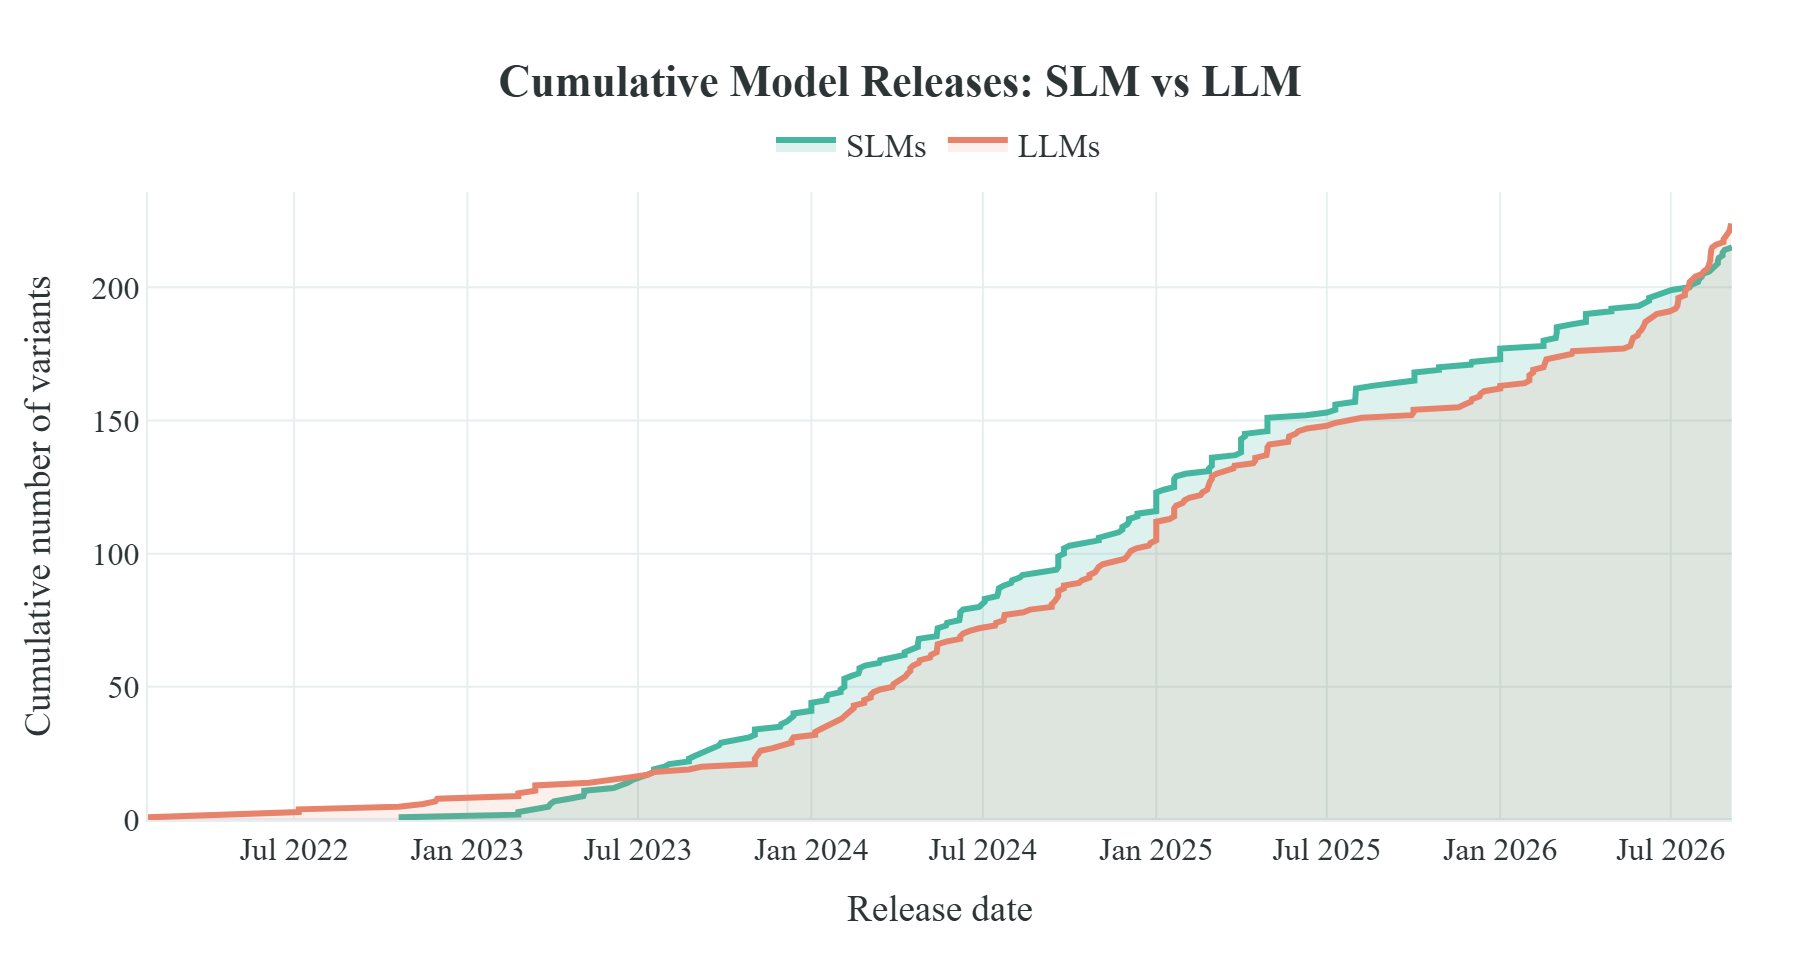
\includegraphics[width=\linewidth, alt={Two panels. Left: stacked bars of documented variants released per year from 2023 to 2026, split into small language models and small-active-parameter mixtures of experts; small language models peak at 71 in 2024 and fall to 51 in 2025 and 22 in 2026 to September, while small-active mixtures of experts rise to 19 in 2026. Right: cumulative release curves for small language models (reaching 179), small-active mixtures of experts (reaching 30), and large language models of disclosed size (reaching 104).}]{paper_combined_cumulative_releases.png}
  \caption{Documented variants by class: releases per year (left; 2026 to 4~September) and cumulative releases (right), from version~3.6 of the released inventory. SLMs meet both C1 and C2; small-active-parameter MoEs meet C1 only and are plotted separately; the comparison curve counts the 104 records of disclosed size that fail C1. The 119 records of undisclosed size cannot be classified and are not plotted.}
  \Description{Two panels. Left: stacked bars of documented variants released per year from 2023 to 2026, split into small language models and small-active-parameter mixtures of experts; small language models peak at 71 in 2024 and fall to 51 in 2025 and 22 in 2026 to September, while small-active mixtures of experts rise to 19 in 2026. Right: cumulative release curves for small language models (reaching 179), small-active mixtures of experts (reaching 30), and large language models of disclosed size (reaching 104).}
  \label{fig:cumulative_releases}
\end{figure}

% ----------------------------------------------------------------
\subsection{Definitions and Terminology}
\label{subsec:intro_definition}

``Small'' is used in the literature to mean at least four different things, so we fix the terms before using them.

\subsubsection{The Operative Definition}
\label{subsubsec:intro_def_operative}

A model is a \emph{small language model} in this survey when it satisfies both of the following:

\begin{description}
  \item[C1 (compute envelope)] It is an autoregressive decoder-only model (attention, state-space, or a hybrid) whose \emph{active} parameter count per generated token is at most roughly twenty billion.
  \item[C2 (storage envelope)] Its \emph{total} parameter count is also at most roughly twenty billion, so that its weights, about 11--15~GB at the 4.4--5.8 effective bits per weight of common 4-bit formats (\suppsec~\ref{subsec:reported_quantization}), can be stored and downloaded like a consumer application and, on runtimes that keep every weight in memory, held on one 16--24~GB consumer GPU or laptop.
\end{description}

\begin{figure}[t]
\centering
\footnotesize
\definecolor{dfInk}{HTML}{34404A}
\definecolor{dfBlue}{HTML}{7397B8}
\definecolor{dfLav}{HTML}{9B8FB5}
\definecolor{dfApr}{HTML}{D8A879}
\definecolor{dfSlate}{HTML}{A2AAB1}
\begin{tikzpicture}[x=1cm,y=1cm,
  lab/.style={font=\scriptsize, text=dfInk, align=center},
  pt/.style={circle, fill=dfInk, inner sep=1.1pt},
  ptl/.style={font=\tiny\itshape, text=dfInk!80}]
% regions (axes: total parameters horizontally, active per token vertically; 20B at 4.0 / 2.2)
\fill[dfBlue!18] (0,0) -- (4.0,0) -- (4.0,2.2) -- cycle;
\fill[dfLav!20] (4.0,0) rectangle (8.2,2.2);
\fill[dfApr!22] (4.0,2.2) -- (8.2,2.2) -- (8.2,4.5) -- cycle;
\fill[dfSlate!25] (0,0) -- (8.2,4.5) -- (0,4.5) -- cycle;
% axes, threshold lines, diagonal
\draw[->, dfInk] (0,0) -- (8.5,0) node[below left, lab] {Total parameters (C2: storage)};
\draw[->, dfInk] (0,0) -- (0,4.8) node[above right, lab, anchor=south west] {Active parameters per token (C1: compute)};
\draw[dashed, dfInk!70] (4.0,0) -- (4.0,4.5);
\draw[dashed, dfInk!70] (0,2.2) -- (8.2,2.2);
\draw[dfInk!70] (0,0) -- (8.2,4.5);
\node[lab, below] at (4.0,0) {about 20B};
\node[lab, left] at (0,2.2) {about 20B};
\node[lab, rotate=28.8, above, font=\tiny] at (6.6,3.62) {dense: active $=$ total};
% region labels
\node[lab] at (3.0,1.2) {\textbf{SLM}\\179};
\node[lab] at (6.6,0.9) {\textbf{Small-active MoE}\\30 (17 above 100B total)};
\node[lab] at (7.3,2.85) {\textbf{LLM}\\104};
\node[lab, text=dfInk!75] at (1.7,3.4) {not possible\\(active $>$ total)};
% example models
\node[pt] at (2.75,0.42) {}; \node[ptl, left] at (2.72,0.42) {Granite 4.0 Tiny};
\node[pt] at (4.75,1.15) {}; \node[ptl, above] at (4.75,1.17) {Qwen3-30B-A3B};
\node[pt] at (5.65,1.6) {}; \node[ptl, above] at (5.65,1.62) {119B total, 6.5B active};
% undisclosed box
\node[draw=dfSlate!90, fill=dfSlate!12, rounded corners=2pt, lab, text width=21mm, inner sep=3pt] at (10.1,2.2) {\textbf{Undisclosed size}\\119\\cannot be placed on either axis};
\end{tikzpicture}
\caption{The two bounds of the definition. C1 bounds active parameters per token, which set per-token compute, latency, and energy; C2 bounds total parameters, which set storage and download size (and resident memory when every weight is kept in memory). Dense models lie on the diagonal. Counts are inventory records (version~3.6); example points are illustrative placements on schematic logarithmic axes, not a plot of the inventory.}
\Description{Schematic plane with total parameters on the horizontal axis and active parameters per token on the vertical axis, each with a threshold at about twenty billion. The region where both are below the threshold is labelled SLM, 179; below the active threshold but above the total threshold is small-active mixture of experts, 30, of which 17 exceed 100B total; above the active threshold is LLM, 104; above the diagonal is not possible. Example points: Granite 4.0 Tiny in the SLM region, Qwen3-30B-A3B and a 119B-total, 6.5B-active model in the small-active region. A separate box holds 119 records of undisclosed size.}
\label{fig:slm_definition}
\end{figure}

C1 bounds per-token compute, latency, and energy (Figure~\ref{fig:slm_definition}). C2 bounds storage and download size, and resident memory only on runtimes that keep all weights resident: runtimes that stream weights or experts from flash \citep{alizadeh2024llmflash}, as Apple's 20B-total, 1--4B-active on-device model does \citep{apple2026afm3}, decouple residency from total size, so for such models resident memory has to be reported separately rather than read off C2. The two conditions coincide for dense models, which is why a single threshold has sufficed in most prior work, but they come apart for \gls{moe} models: a 119B-total model that activates 6.5B parameters per token has the per-token cost of a 6.5B model and the storage cost of a 119B one. The twenty-billion figure is a convention, not a natural kind. Applied to the records of disclosed size in the released file, a bound of 10B, 13B, 20B, or 32B total parameters would admit 143, 160, 179, or 209 of them respectively, and every record carries its counts so that any other threshold can be applied.

\subsubsection{Four Distinguished Terms}
\label{subsubsec:intro_def_terms}

\begin{description}
  \item[\gls{slm}] A model satisfying C1 and C2. Every deployment, storage, and on-device claim in this paper applies to this class.
  \item[Compact model] An \gls{slm} at or below roughly 3B total parameters, whose 4-bit weights fit in about 2~GB of the 4--8~GB a current phone leaves to applications. Most documented phone deployments use this band; the exceptions keep part of the model off the accelerator, through per-layer embeddings (Gemma~3n and Gemma~4 E-series) or flash-resident experts (Apple's third-generation on-device model).
  \item[Edge model] A model, of any size, for which the developer documents and ships an artifact for phone-, single-board-computer-, or \gls{npu}-class hardware. ``Edge'' is a claim about the deployment target, not about parameter count.
  \item[Small-active-parameter \gls{moe}] A model satisfying C1 but not C2. These have \gls{slm}-like per-token cost and \gls{llm}-like storage cost. They are recorded in the inventory but counted, plotted, and discussed separately, and are excluded from every claim about storage, download size, resident memory, or on-device feasibility. The class is wide: 17 of its 30 members exceed 100B total parameters, so it includes frontier-scale models such as Llama~4 Maverick and Qwen3.5-397B-A17B as well as 21--35B models.
\end{description}

The inventory holds 179 \glspl{slm} and 30 small-active-parameter \glspl{moe}; wherever this paper counts \glspl{slm}, it means the 179. Per-layer-embedding ``effective'' sizes (Gemma~3n, Gemma~4 E2B/E4B) are not sparse activation, so C1 is evaluated on those models' total counts. The unit counted is the \emph{variant}: a separately released artifact of one size within a family, which may be a distinct post-training or domain specialization released as its own repository (for example Phi-4 and Phi-4-reasoning), with checkpoint revisions of the same artifact counted once. Counted instead by distinct family and size, the 179 \glspl{slm} are 136 family--size pairs. \suppsec~\ref{supp:definitions} lists the reporting dimensions the inventory records and their coverage (total parameters 209/209, context length 135/209, peak runtime memory not reported by vendors), and the artifact vocabulary.

\subsection{The Agentic Turn and the Thesis}
\label{subsec:intro_agentic}
\label{subsec:intro_thesis}

A large share of model calls is now issued by AI agents: control loops in which a model is called repeatedly to choose a tool, fill its arguments, extract a field, classify an intent, or check a result \citep{belcak2025slm_agentic,chen2024mas_survey}. Many such calls are narrow, repetitive, and format-constrained. \citet{belcak2025slm_agentic} argue that for these calls \glspl{slm} should be the default, and \citet{sharma2025slm_agentic} survey the evidence and propose an \gls{slm}-default, \gls{llm}-fallback design. We state the position as a conditional hypothesis whose terms can be measured.

\begin{quote}
\textbf{H (default hypothesis).} Consider a type of language-model call inside an agent with the following properties.
\begin{description}
  \item[H1 (bounded)] The output is a tool selection, a record conforming to a fixed schema, a label from a fixed set, or a local edit of a few lines.
  \item[H2 (recurrent)] The expected number of such calls over the planning horizon, $N$, exceeds the break-even volume
  \begin{equation}
    N^{*} = \frac{F}{\,c_L - (a\,c_S + c_V + e\,c_L)\,},
    \label{eq:breakeven}
  \end{equation}
  where $F$ is the one-time and maintenance cost of specializing for the call type, $c_L$ and $c_S$ are the per-call serving costs of the large and the small model, $a \ge 1$ is the expected number of small-model attempts per call, $c_V$ is the per-call cost of the check, and $e$ is the escalation rate. If the denominator is not positive, specialization never pays.
  \item[H3 (short-context)] The input needed fits within a few thousand tokens without retrieval over a large corpus.
  \item[H4 (checkable)] Two checks exist at a cost small relative to $c_L$: a \emph{validity} check (H4a: schema validation, parsing, type checking), and a \emph{correctness} check (H4b: an executor with observable effects, a unit test, a constraint solver, or a lookup against a reference) that detects outputs which are well formed but wrong. Validity checking alone does not satisfy H4.
\end{description}
For such a call type, a specialized \gls{slm} is the appropriate default: the call goes to the \gls{slm} first and is escalated to a frontier \gls{llm} when a check fails. ``Appropriate default'' means that the \gls{slm}-first system is non-inferior to an all-\gls{llm} system in task success, within a margin $\delta$ fixed in advance, at a lower cost per completed task than every comparator of Section~\ref{subsec:challenges_verification}.
\end{quote}

\begin{figure}[t]
\centering
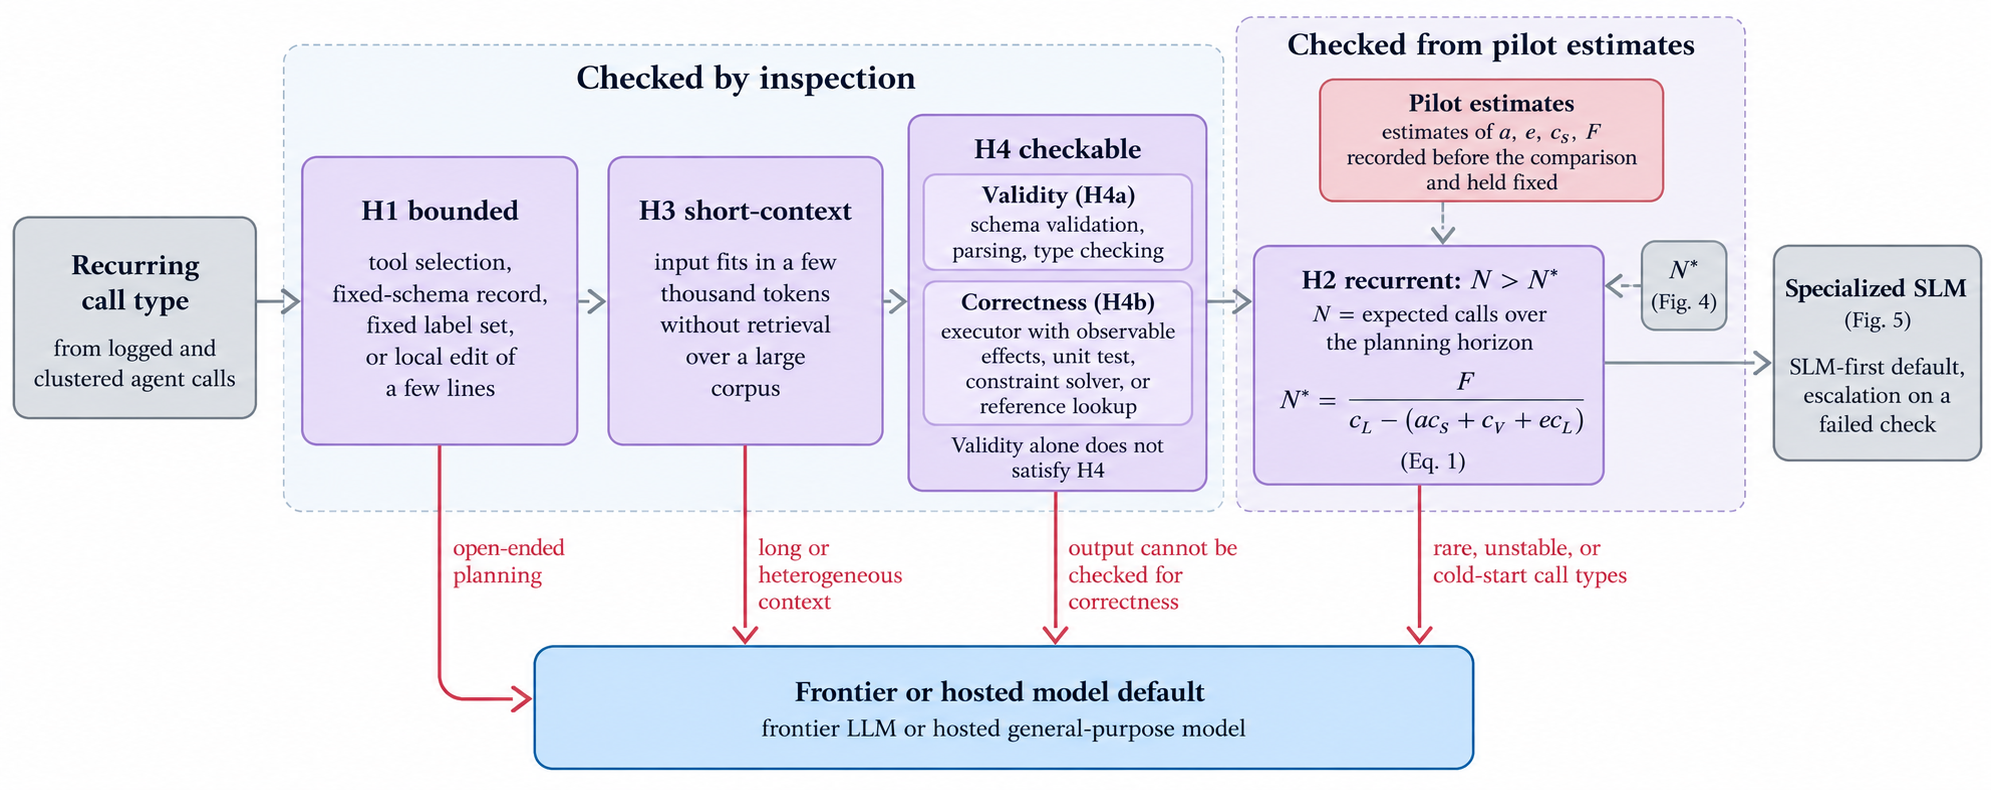
\includegraphics[width=\linewidth, alt={Left-to-right flow: a recurring call type passes through gates H1 bounded, H3 short-context, H4 checkable (validity and correctness), and H2 recurrent, and if all pass reaches specialized SLM as the default. From each gate a downward arrow labelled open-ended planning, long context, uncheckable output, or rare or unstable leads to a box reading frontier or hosted model as default. Labels mark H1, H3, and H4 as checked by inspection and H2 as checked from pilot estimates.}]{fig03-hypothesis-conditions.png}
\caption{Assessing one recurring agent call type against hypothesis~H at design time. H1, H3, and H4 are checked by inspecting the call type; H2 is checked against pilot estimates recorded before any comparison. A call type that passes every condition defaults to a specialized SLM with escalation on a failed check (Figure~\ref{fig:hetero_agent}); a failure at any condition, labelled with the workload class that typically fails there (Section~\ref{subsec:agentic_counterexamples}), leaves a frontier or hosted model as the default.}
\Description{Left-to-right flow: a recurring call type passes through gates H1 bounded, H3 short-context, H4 checkable (validity and correctness), and H2 recurrent, and if all pass reaches specialized SLM as the default. From each gate a downward arrow labelled open-ended planning, long context, uncheckable output, or rare or unstable leads to a box reading frontier or hosted model as default. Labels mark H1, H3, and H4 as checked by inspection and H2 as checked from pilot estimates.}
\label{fig:hypothesis_conditions}
\end{figure}

H1, H3, and H4 can be checked by inspecting a call type before any model is trained (Figure~\ref{fig:hypothesis_conditions}). H2 cannot be checked from first principles, because $a$, $e$, and $c_S$ depend on the specialized model: it is assessed from pilot estimates recorded before the comparison and held fixed, so that a failed comparison cannot be reclassified afterwards as a failure of H2. H is refuted for a workload class meeting H1--H4 if a pre-registered comparison of the kind specified in Section~\ref{subsec:challenges_verification} finds the \gls{slm}-first system inferior by more than $\delta$, or more costly per completed task than any comparator, and it is rejected as a general design rule if it fails on a majority of at least three pre-registered workloads with distinct call types. It does not claim that \glspl{slm} match frontier models in general, that agents can dispense with large models, or any particular share of agent traffic meeting H1--H4. Section~\ref{subsec:agentic_counterexamples} sets out the workload classes for which the conditions fail. Section~\ref{subsec:agentic_evidence} grades the evidence bearing on H: it is strongest for per-call competence of specialized sub-10B models, contested for end-to-end success, and absent for cost per completed task in an \gls{slm}-first agent.

\subsection{Scope and Contributions}
\label{subsec:intro_gap}

Existing \gls{slm} surveys \citep{lu2024slmsurvey,vannguyen2024slm_survey,wang2024comprehensive,gupta2025slmsurvey} provide taxonomies, technique reviews, and measurements but treat agentic deployment only in passing. The agentic case has been made as a position \citep{belcak2025slm_agentic,tian2026edgeagents} and as a survey \citep{sharma2025slm_agentic}, which already proposes \gls{slm}-default, \gls{llm}-fallback systems with verifier cascades, cost per successful task as the deciding metric, and limits where fallback remains necessary. We share that direction. This paper adds the following:

\begin{description}
  \item[A two-bound definition] that separates per-token cost (C1) from storage cost (C2) and so treats mixtures of experts consistently (Section~\ref{subsec:intro_definition}).
  \item[A verified inventory] of 179 \glspl{slm} and 30 small-active-parameter \glspl{moe} (2023--2026), in which every record's developer source has been checked and every inclusion decision is recorded with its reason, released with the scripts that apply the rule and generate every table and figure (\suppsec~\ref{supp:method}).
  \item[An audit of the vendor evaluation record] that quantifies why a cross-model table cannot be built from it: for the 14 cohort models of the four largest vendors, no benchmark is reported for all of them, and no stated protocol is shared by more than five (Section~\ref{sec:reported}).
  \item[A compression review] that reports reductions along separate axes of parameters, memory, training compute, and latency (Section~\ref{sec:compression}).
  \item[An operational version of the agentic hypothesis] with a break-even condition that includes retries, checking, and escalation, a correctness requirement on the check, graded agent-specific evidence including contrary results, and the workload classes for which it fails (Section~\ref{sec:agentic}).
  \item[A falsification design] that specifies comparators, the statistical decision rule, and the sample size needed to decide H for a workload, with five further verification studies (Section~\ref{sec:challenges}).
\end{description}

\subsection{Survey Method and Sources}
\label{subsec:intro_method}

This is a structured narrative survey, not a systematic review; its aims are representative coverage of the design space, a verified inventory, and an audit of a defined cohort. It addresses five research questions: the design space of \glspl{slm} released 2023--2026 (RQ1); which compression techniques pay in the sub-10B regime, along which axis, and at what quality cost (RQ2); what the vendor evaluation record can and cannot support (RQ3); what agent-specific evidence says about small models (RQ4); and under which conditions a small model is the appropriate default inside an agent (RQ5).
\label{subsubsec:intro_rqs}
\label{subsubsec:intro_search}

\emph{Model inventory (RQ1).} A seed list compiled in March 2026 from public model listings and aggregators, 205 of whose records were compiled with the assistance of a large language model, was updated on 5~September 2026 against the OpenRouter catalogue and vendor announcements, and every record was then classified against C1 and C2. On 8~October 2026 every record's developer source was checked through the Hugging Face Hub API: 197 of the 209 included records link an existing repository owned by the developer, and the other 12 link the developer's own announcement, paper, or code repository. Twelve records first sourced from an aggregator or a press article were re-sourced to the developer, and one for which no developer source exists was excluded. C1, C2, and inclusion criteria M1 (a developer source states size and architecture) and M4 (a dated release) are computed from recorded fields by a released script; the exclusions of derivative fine-tunes, API aliases, and encoder-decoder models are named editorial decisions listed in that script. The released file records, per record, the check, its date, and the Hub parameter count where available. Coverage is strongest for developers that publish on the Hub. \suppsec~\ref{supp:method} gives the criteria, the seven excluded records, and the count history.

\emph{Technique literature (RQ2, RQ4, RQ5).} Works were identified from the prior surveys cited above, by backward and forward citation tracing, and by targeted searches of arXiv and the ACL Anthology, last run on 8~October 2026 for agent-specific evaluation, routing, function calling, and cost-per-outcome measurement. Screening decisions were not recorded for this stream, so statements that we ``found no'' study are bounded by that search.

\emph{Evaluation record (RQ3).} For each model of the 18-model cohort, the primary release document and official model card were consulted; the coverage ledger of Section~\ref{subsec:reported_overall} was transcribed from them on 8~October 2026. No benchmark was executed for this survey.

\emph{Appraisal.} Each empirical claim carries an evidence grade (Section~\ref{subsec:reported_grading}) reflecting its design and the independence of its source.
\label{subsubsec:intro_inclusion_summary}

\subsection{Organization}
\label{subsec:intro_organization}

Section~\ref{section:background} reviews related work. Section~\ref{sec:taxonomy} presents the taxonomy, Section~\ref{sec:compression} compression, Section~\ref{sec:reported} the evaluation record and the grading scheme, and Section~\ref{sec:deployment} deployment. Section~\ref{sec:agentic} assesses H on agent-specific evidence and states its counterexamples. Section~\ref{section:discussion} discusses implications, applications, and limitations, Section~\ref{sec:challenges} sets out open problems and the verification agenda, and Section~\ref{section:conclusion} concludes. The electronic supplement (\suppsec~\ref{supp:definitions} to \suppsec~\ref{supp:last}) holds the reporting dimensions, inclusion criteria and released artifacts, detailed technique reviews, the audit ledger, reference tables, domain applications, and the generated variant inventory.

\section{Related Work and Research Gaps}
\label{section:background}

\subsection{From Scaling to Small Models}
\label{subsec:background_evolution}
\label{subsec:background_techniques}
\label{subsec:background_families}

The Transformer \citep{vaswani2017attention} and the pre-train-then-adapt paradigm \citep{devlin2019bert,brown2020gpt3} led to a scaling race that the Chinchilla study \citep{hoffmann2022chinchilla} partly redirected: a 70B model trained on 1.4~trillion tokens outperformed the 280B Gopher, implying that most large models were undertrained and that smaller, longer-trained models could match them. Subsequent families pushed this further at small scale through curated and synthetic data \citep{gunasekar2023phi1,abdin2024phi3}, distillation from larger teachers \citep{gemma2024,team2025gemma3}, and pruning plus distillation from a larger sibling, as for Llama~3.2's 1B and 3B edge models \citep{meta2024llama32}. Three bodies of technique underlie the current generation: distillation and synthetic-data training \citep{hinton2015distilling,gunasekar2023phi1}; post-training compression and parameter-efficient adaptation \citep{frantar2023gptq,lin2024awq,hu2022lora,dettmers2023qlora}; and on-device runtimes \citep{gerganov2023llamacpp,meta2024executorch,mlc2024}. Sections~\ref{sec:compression} and~\ref{sec:deployment} review them, and \suppsec~\ref{supp:families} and~\ref{supp:background} summarize the principal families and the longer background.

\subsection{LLM--SLM Collaboration and Agentic Systems}
\label{subsec:background_collab}

A line of work studies how small and large models cooperate \citep{chen2024role_small,chen2025collab_survey}. Cascades and routers are the most relevant to agents: FrugalGPT \citep{chen2023frugalgpt} learns a cascade over commercial APIs, Hybrid~LLM \citep{ding2024hybridllm} routes by predicted difficulty, AutoMix \citep{aggarwal2024automix} escalates on self-verification, RouteLLM \citep{ong2024routellm} learns from preference data, RouterBench \citep{hu2024routerbench} benchmarks routers on 405K inference outcomes, and Division-of-Thoughts \citep{division_of_thoughts_2025} routes sub-questions between an on-device and a cloud model. Speculative decoding \citep{leviathan2023speculative,chen2023specsampling} uses a small model to accelerate a large one without delegating answers. On the agentic side, function-calling data pipelines report specialized sub-10B models among the leading entries of the Berkeley Function-Calling Leaderboard \citep{liu2024apigen,liu2025toolace,zhang2024xlam}, and agent evaluation has begun to report cost alongside accuracy \citep{kapoor2024agentsmatter,kapoor2025hal,erol2025costofpass}.

\subsection{Gaps in Existing Literature}
\label{subsec:background_gaps}

General \gls{slm} surveys \citep{lu2024slmsurvey,vannguyen2024slm_survey,wang2024comprehensive} provide technique taxonomies, application coverage, and in the case of \citet{lu2024slmsurvey} a measurement study of 70 models; \citet{gupta2025slmsurvey}, updated in 2026, survey about 160 papers on 1--8B models. None separates active from total parameters or foregrounds agentic deployment. \citet{srivastava2025thinkslm} benchmark 72 small models on 17 reasoning benchmarks with three repeats, including models derived by quantization, pruning, and distillation, and find that reasoning tracks training method and data more than scale and that quantization preserves reasoning while pruning disrupts it; it is the closest thing in the literature to the controlled evaluation whose absence Section~\ref{sec:reported} documents, but covers reasoning only. \citet{feng2025efficient_reasoning_survey} survey efficient reasoning, and \citet{chen2024mas_survey} survey multi-agent systems by application.

Two works state the agentic case directly. \citet{belcak2025slm_agentic} argue it as a position, with a conversion algorithm and estimates of how much agent traffic small models could handle, and \citet{tian2026edgeagents} argue that personal agents must move to the edge. The closest prior work is the survey of \citet{sharma2025slm_agentic}. It reviews 1--12B (occasionally about 20B) models for agentic workloads, proposes an \gls{slm}-default, \gls{llm}-fallback architecture with uncertainty-aware routing, retries, and verifier repair (their Section~VIII), proposes cost per successful task as the deciding metric, and names where large models still win: open-domain synthesis, complex multi-hop reasoning, safety-critical judgment, and long-context work (their Section~XI). We share that design and metric. It does not separate active from total parameters, grade its evidence or report contrary results, examine whether the vendor evaluation record supports comparison, or state a decision rule under which its position would be refuted, and its estimate that cost per successful task falls 10--30$\times$ (their Section~X) is not a reported measurement. Those are the points on which this paper differs: the C1/C2 definition, the verified inventory, the quantified audit of the evaluation record, graded evidence including contrary results, a break-even condition that includes retries, checking, and escalation together with a correctness requirement on the check, and a falsification design with comparators, a decision rule, and a sample size. Table~\ref{tab:survey_compare} summarizes the positioning.

\begin{table}[t]
\centering
\caption{Coverage of this survey relative to prior surveys and position papers (Y~full, P~partial, --~absent), as judged by the present authors from each work's text (grade~\evD). \emph{Active/total}: separates active from total parameters. \emph{Evaluation critique}: analysis of whether the reporting record supports cross-model comparison. \emph{Graded evidence}: an explicit strength-of-evidence grade per claim. \emph{Agentic focus}: small models inside agents as a primary topic. \emph{Decision rule}: a stated condition under which the position is refuted.}
\label{tab:survey_compare}
\footnotesize
\adjustbox{max width=\linewidth}{%
\begin{tabular}{lccccccc}
\toprule
\textbf{Work} & \textbf{Taxonomy} & \textbf{Compression} & \textbf{Active/} & \textbf{Evaluation} & \textbf{Graded} & \textbf{Agentic} & \textbf{Decision} \\
 & & & \textbf{total} & \textbf{critique} & \textbf{evidence} & \textbf{focus} & \textbf{rule} \\
\midrule
\citet{lu2024slmsurvey}            & Y & P & -- & P & -- & -- & -- \\
\citet{vannguyen2024slm_survey}    & Y & Y & -- & -- & -- & -- & -- \\
\citet{wang2024comprehensive}      & Y & Y & -- & -- & -- & P & -- \\
\citet{gupta2025slmsurvey}         & Y & P & -- & -- & -- & -- & -- \\
\citet{srivastava2025thinkslm}     & P & P & -- & Y & -- & -- & -- \\
\citet{belcak2025slm_agentic}      & -- & -- & -- & P & -- & Y & -- \\
\citet{tian2026edgeagents}         & -- & -- & -- & -- & -- & Y & P \\
\citet{sharma2025slm_agentic}      & P & P & -- & -- & -- & Y & -- \\
\textbf{This survey}               & Y & Y & Y & Y & Y & Y & Y \\
\bottomrule
\end{tabular}%
}
\end{table}

% ================================================================
% Section: Taxonomy of Small Language Models
% ================================================================

\section{A Faceted Taxonomy of Small Language Models}
\label{sec:taxonomy}

\subsection{The Scheme}
\label{subsec:taxonomy_scheme}

We index the \gls{slm} design space along four \emph{primary} facets, architecture, training strategy, modality, and application domain (Figure~\ref{fig:taxonomy}), and five \emph{secondary} facets that govern adoption: licensing, data transparency, safety alignment, reasoning mode, and deployment target (Table~\ref{tab:taxonomy_facets} in \suppsec~\ref{supp:tables}). The facets are \emph{separately observable}, in that each can be read off a model's primary source, but they are \emph{not orthogonal}: pruning-plus-distillation presupposes a dense teacher, and a vision encoder ties modality to architecture. The scheme is also \emph{multi-label}: Gemma~3 is distilled \emph{and} trained on a curated corpus, Granite~4.0 is a hybrid state-space model \emph{and} a mixture of experts. It is an indexing scheme illustrated with exemplars, not a partition of the inventory. The released inventory records per variant the fields its sources state directly (modality, access, license, dense or mixture-of-experts, post-training status, context length), and the figures are drawn from those fields; architecture and training facets are assigned in this paper to representative models only. The application-domain facet is the weakest of the four, since it usually describes use rather than the artifact, so we assign it only when the developer trained the released artifact for a domain and says so.

\begin{figure}[t]
\centering
\footnotesize
% Palette shared with the generated figures (source/scripts/generate_figures_v2.py).
\definecolor{txInk}{HTML}{34404A}
\definecolor{txSlate}{HTML}{A2AAB1}
\definecolor{txIndigo}{HTML}{7397B8}
\definecolor{txOcean}{HTML}{D8A879}
\definecolor{txTeal}{HTML}{79A88E}
\definecolor{txCoral}{HTML}{9B8FB5}
\newcommand{\txax}[2]{{\normalsize\bfseries\color{#1!88!black}#2}}
\newcommand{\txcat}[1]{{\scriptsize\bfseries\color{txInk}#1}}
\newcommand{\txsep}{{\color{txSlate}\,\textendash\,}}
\newcommand{\txex}[1]{{\scriptsize\itshape\color{txSlate}#1}}
\begin{tikzpicture}[
  panel/.style={draw=#1!55, line width=0.7pt, rounded corners=3pt, inner sep=5pt,
                text width=0.455\linewidth, align=left, fill=#1!7},
  node distance=3mm and 3mm,
]
\node[panel=txIndigo] (arch) {%
  \txax{txIndigo}{1.\ Architecture}\\[2pt]
  \txcat{Dense transformer}\txsep GQA, RoPE, gated FFN\\ \txex{Phi-4-mini, Qwen3, SmolLM3, Gemma 3}\\[1pt]
  \txcat{Mixture-of-experts}\txsep sparse activation\\ \txex{Granite 4.0 Tiny; small-active MoE: Mixtral, Qwen3-30B-A3B}\\[1pt]
  \txcat{Hybrid SSM/attention}\txsep linear-time\\ \txex{Falcon-H1, Granite 4.0, Nemotron Nano 2}%
};
\node[panel=txOcean, right=of arch] (train) {%
  \txax{txOcean}{2.\ Training strategy}\\[2pt]
  \txcat{From scratch}\txsep curated / synthetic data\\ \txex{Phi, Qwen3, SmolLM3}\\[1pt]
  \txcat{Distillation}\txsep transfer from a larger teacher\\ \txex{Gemma 3/4, DeepSeek-R1-Distill, Phi-4-mini-reasoning}\\[1pt]
  \txcat{Pruning + distillation}\txsep shrink a larger model\\ \txex{Minitron, Sheared-LLaMA, Llama 3.2 1B/3B}%
};
\node[panel=txTeal, below=of arch] (mod) {%
  \txax{txTeal}{3.\ Modality}\\[2pt]
  \txcat{Text-only}\txsep majority of SLMs\\ \txex{Mistral 7B, SmolLM3, Qwen3}\\[1pt]
  \txcat{Vision--language}\txsep image encoder added\\ \txex{Phi-3-vision, Gemma 3 (4B+), PaliGemma}\\[1pt]
  \txcat{Text + vision + audio}\txsep one sub-10B model\\ \txex{Gemma 3n, Gemma 4, Voxtral Mini (audio)}%
};
\node[panel=txCoral, below=of train] (dom) {%
  \txax{txCoral}{4.\ Application domain}\\[2pt]
  \txcat{General-purpose}\txsep broad benchmarks\\ \txex{Phi, Gemma, Llama, Qwen, Mistral}\\[1pt]
  \txcat{Healthcare}\txsep clinical text\\ \txex{Meerkat, OptimCLM (encoders)}\\[1pt]
  \txcat{Code / multilingual}\txsep domain corpora\\ \txex{StarCoder2, DeepSeek-Coder, Aya 23}%
};
\end{tikzpicture}
\caption{The four primary facets of the taxonomy. Facets are separately observable but not orthogonal, and assignment is multi-label. Representative models are italicised; \suppsec~\ref{supp:taxonomy} develops each facet and Table~\ref{tab:taxonomy_summary} gives the tabular form.}
\Description{A two-by-two arrangement of four labelled panels, one per primary taxonomy facet: architecture, training strategy, modality, and application domain. Each panel lists three categories with a short defining characteristic and representative models.}
\label{fig:taxonomy}
\end{figure}

% ----------------------------------------------------------------
\subsection{Architecture}
\label{subsec:taxonomy_architecture}

\emph{Dense transformers} remain the majority, from SmolLM2-135M \citep{allal2025smollm2} to 7--14B models. The recurring refinements are grouped-query attention \citep{ainslie2023gqa}, which shrinks the \gls{kv} cache by the ratio of query to \gls{kv} heads; rotary position embeddings with an enlarged base or rescaling for long context; and gated feed-forward layers (SwiGLU in most families, GeGLU in Gemma). Among \glspl{slm} whose records state a context length, the median grew from 2K tokens in 2023 ($n=5$) to 16K in 2024 ($n=39$) and 128K in 2025 ($n=46$) and 2026 ($n=20$); coverage is thin for 2023, so the starting point is uncertain (\suppsec~\ref{supp:figures}).

\emph{Mixtures of experts} \citep{shazeer2017moe,fedus2022switch} decouple total from active parameters, and they sit on the fault line that C2 marks. Qwen3-30B-A3B \citep{qwen3_2025} costs about what a 3B dense model costs per token but needs 17--22~GB of 4-bit weight storage, so it is a small-active-parameter \gls{moe} in this paper, not an \gls{slm}; Granite~4.0 Tiny (about 7B total, 1B active) \citep{granite4_2025} satisfies both conditions. The 2026 releases concentrated in this class, with Nemotron~3.5 Lightning (30B/3B), Laguna XS~2.1 (33B/3B), Ling~3.0 Flash (124B/5.1B), and DeepSeek V4 Flash (284B/13B) appearing between June and August 2026.

\emph{Hybrid state-space models} combine attention with linear-time state-space layers \citep{gu2023mamba}. Jamba \citep{lieber2024jamba} interleaves Mamba and attention blocks and reports a \gls{kv} cache eight times smaller than Mixtral's at 256K context; Falcon-H1 \citep{falconh1_2025}, Granite~4.0 \citep{granite4_2025}, Nemotron Nano~2 \citep{nvidia2025nemotron_nano2}, and the Qwen3.5 small series \citep{qwen3_5_2026} brought the design to production at small scale in 2025--2026. \suppsec~\ref{supp:taxonomy} gives the architectural detail for each class.

\subsection{Training Strategy, Modality, and Domain}
\label{subsec:taxonomy_training}
\label{subsec:taxonomy_modality}
\label{subsec:taxonomy_domain}

Three training routes recur and are often combined: training from scratch on curated or synthetic data (Phi, SmolLM, Qwen), distillation from a larger teacher (Gemma, the DeepSeek-R1 students, Phi-4-mini-reasoning), and pruning a larger model followed by distillation (Minitron, Sheared-LLaMA, Llama~3.2 1B and 3B). Text-only models still dominate the inventory, vision--language models are common at 2--12B, and audio and natively multimodal mobile models (Qwen2.5-Omni, Gemma~3n and~4, Voxtral Mini) grew in 2025--2026 (\suppsec~\ref{supp:figures}). Most \glspl{slm} are released as general-purpose models; developer-trained domain models concentrate in code, healthcare, and multilingual use. \suppsec~\ref{supp:taxonomy} lists representative models for each category.

% ================================================================
% Section: Model Compression Techniques for \glspl{slm}
% Merged from main (2).tex — Section IV + sections/background.tex
% ================================================================

\section{Model Compression Techniques for SLMs}
\label{sec:compression}

Model compression is central to the \gls{slm} ecosystem: it is the primary pathway for reducing large pre-trained models to sizes deployable on edge hardware, and it provides a complementary route to training-from-scratch. The principal techniques are knowledge distillation, quantization, and pruning; in practice, compound pipelines combining all three have become the state of the art.

\subsection{How Compression Results Are Reported Here}
\label{subsec:compression_reporting}

Comparisons of compression techniques are routinely presented as a single
``compression ratio'' set against a single ``accuracy retention'' percentage. An
earlier version of this survey did the same, and the presentation does not
survive scrutiny, so we set out here why and what replaces it.

\emph{There is no single compression ratio.} Quantization reduces bits per
weight, leaving the parameter count untouched; pruning reduces the parameter
count, and reduces memory only where the sparsity pattern is one the runtime can
actually exploit; distillation reduces the parameter count of the student but is
better understood as reducing the training compute needed to reach a given
quality, since a distilled 4B model and a from-scratch 4B model have the same
deployment cost. Collapsing these into one number equates quantities that trade
off against different budgets. Distillation in particular has no well-defined
universal ratio at all: the student's size is chosen by the practitioner, so
``$10$--$100\times$'' describes a range of design choices in the literature, not a
property of the method.

\emph{There is no baseline-free accuracy retention.} A statement that 4-bit
quantization retains ``about 96\%'' of accuracy is uninterpretable without the
baseline precision, the model, the model's size, the task, the metric, and the
rule by which per-task retentions were aggregated. The dependence on each of
these is large: retention under \gls{ptq} falls with model size
\citep{slmquant2025}, differs by task family, with mathematical and multi-step
reasoning degrading faster than knowledge recall, and differs by method at
matched bit-width \citep{lin2024awq}. A single band averages across all of that
variation and then presents the average with two significant figures.

We therefore replace the single table with two. Table~\ref{tab:compression_axes}
separates the reductions each technique delivers along five distinct axes, which
are not interchangeable and are not summed. Table~\ref{tab:compression_quality}
reports what the reviewed literature establishes about quality cost, stated as a
direction and a scope condition with the source attached, rather than as a
number without a baseline. Where the literature supports a numeric claim under
stated conditions, the number appears in the text with its conditions; where it
does not, no number is given, and Section~\ref{subsec:challenges_verification}
specifies the experiment that would supply one.

\begin{table}[t]
\caption{What each compression technique reduces, by axis. Entries are what the technique does by construction, not measurements. ``Parameters'' counts stored weights; ``memory'' is realized weight footprint on a runtime that can exploit the format; ``training compute'' is the cost of producing the compressed artifact relative to training an equivalent model from scratch; ``latency'' is decode-time speedup on memory-bandwidth-bound hardware. A dash means the technique does not act on that axis.}
\label{tab:compression_axes}
\centering
\footnotesize\adjustbox{max width=\linewidth}{%
\begin{tabular}{@{}lp{1.7cm}p{1.9cm}p{2.1cm}p{2.4cm}p{2.1cm}@{}}
\toprule
\textbf{Technique} & \textbf{Parameter reduction} & \textbf{Weight-memory reduction} & \textbf{Training-compute reduction} & \textbf{Decode latency effect} & \textbf{Retraining required} \\
\midrule
PTQ, 8-bit          & ---            & $2\times$ vs.\ FP16 & ---  & Proportional to bandwidth saved & No \\
PTQ, 4-bit          & ---            & $3.2$--$3.4\times$ realized (Table~\ref{tab:memory_footprint}) & --- & Proportional to bandwidth saved, batch~1 & No \\
PTQ, 2-bit          & ---            & ${\sim}6\times$ realized & --- & As above & No; \gls{qat} in practice \\
Unstructured pruning, 50\% & $2\times$ & Only on sparse-capable runtimes & --- & None on dense kernels & Calibration only \\
Structured pruning  & Set by target width/depth & Proportional to parameters removed & --- & Proportional to parameters removed & Yes, to recover quality \\
Knowledge distillation & Set by student size & Proportional to student size & Large; the student is trained rather than the teacher & Proportional to student size & Yes, student training \\
Prune + distill + quantize & Set by target & Product of the pruning and quantization factors & $40\times$ reported for Minitron \citep{minitron2024} & Product of the above & Yes \\
\bottomrule
\end{tabular}%
}
\end{table}

\begin{table}[t]
\caption{What the reviewed literature establishes about the quality cost of each technique in the sub-10B regime, with the scope condition under which it was established. Claims are graded by evidence class (Section~\ref{subsec:reported_grading}): \evB~independent evaluation, \evC~vendor- or author-reported, \evD~synthesis across sources by the present authors.}
\label{tab:compression_quality}
\centering
\footnotesize\adjustbox{max width=\linewidth}{%
\begin{tabular}{@{}lp{6.4cm}p{3.2cm}c@{}}
\toprule
\textbf{Technique} & \textbf{What the literature supports} & \textbf{Scope of the evidence} & \textbf{Grade} \\
\midrule
PTQ, 8-bit & Effectively lossless on knowledge and mathematical benchmarks; no consistent degradation reported & Widely reproduced across model families & \evB \\
PTQ, 4-bit & A small but real accuracy cost that grows as model size falls, and is larger on multi-step reasoning than on knowledge recall & Reported for the sub-4B band \citep{slmquant2025} & \evC \\
PTQ, 4-bit, method comparison & \gls{awq} retains more accuracy than GPTQ at matched bit-width by protecting activation-salient channels & Author-reported, with independent reuse \citep{lin2024awq} & \evC \\
PTQ, 2-bit & \gls{ptq} degrades unacceptably; \gls{qat} recovers a meaningful part of the loss, and the margin over \gls{ptq} widens as bit-width falls & Vendor pipelines with full training-stack control \citep{gunter2025afm} & \evC \\
Unstructured pruning, 50\% & Perplexity increase below 1\% at 175B scale in one pass \citep{frantar2023sparsegpt}; the tolerable sparsity falls sharply as the base model shrinks & Established at large scale; extrapolation to sub-4B is not supported & \evC \\
Quantization vs.\ pruning & Quantization preserves fidelity, multilingual perplexity, and reasoning accuracy better than pruning at matched compression; \gls{awq} 4-bit beats 50\% Wanda on 6 of 7 tasks & Controlled study: 6 models, 0.5--3.8B, 7 languages, 7 tasks \citep{kurz2025pruning_vs_quant} & \evB \\
Prune + distill + quantize & A 4B Minitron matches from-scratch 4B models on commonsense, code, and math at $40\times$ less training compute & Single pipeline, single teacher \citep{minitron2024} & \evC \\
Domain compound pipeline & A clinical model under 1B retains reported accuracy within 5\% of its 7B counterpart on ICD coding and discharge summarization & Single study, single domain \citep{hasan2024optimclm} & \evC \\
Fairness under compression & Degradation is uneven across languages and dialects, and pruning is worse than quantization on multilingual tasks & Inferred across two sources \citep{blodgett2020language,kurz2025pruning_vs_quant} & \evD \\
\bottomrule
\end{tabular}%
}
\end{table}

% ----------------------------------------------------------------
\subsection{Knowledge Distillation}
\label{subsec:compression_kd}

\gls{kd} \citep{hinton2015distilling} transfers the ``dark knowledge'' embedded in a teacher model's soft output distribution to a smaller student model. The student is trained to minimize a combination of the standard cross-entropy loss on labeled data and a Kullback--Leibler (KL) divergence loss with respect to the teacher's output logits at a temperature $T > 1$. This approach was pioneered for BERT compression (DistilBERT \citep{sanh2019distilbert}, TinyBERT \citep{jiao2020tinybert}) and has since been substantially extended for generative \glspl{slm}.

\subsubsection{White-Box vs.\ Black-Box KD}

The survey by \citet{yang2024kd_survey} classifies \gls{llm} distillation into two paradigms:

\emph{White-box \gls{kd}} has access to the teacher's intermediate representations. TinyBERT \citep{jiao2020tinybert} pioneered layer-by-layer feature alignment, matching student hidden states, attention matrices, and embedding layers to teacher counterparts via MSE loss. In the decoder-only \gls{llm} setting, this requires pairing student and teacher layers, which is non-trivial when sizes differ substantially, and is computationally expensive but yields superior retention of teacher capabilities.

\emph{Black-box \gls{kd}} uses only the teacher's generated outputs, either token probabilities or free-form text, as the supervision signal. Orca \citep{ho2022orca} exemplifies text-output black-box \gls{kd}: GPT-4 generates step-by-step reasoning traces, which a LLaMA-based student learns to replicate. DeepSeek-R1 \citep{deepseek2025r1} extends this to long chain-of-thought reasoning distillation, producing 7B and 14B students that dramatically outperform identically-sized from-scratch models on mathematical reasoning.

\subsubsection{Chain-of-Thought Distillation}

A particularly productive form of black-box \gls{kd} is \gls{cot} distillation \citep{wei2022cot}: the teacher model generates explicit reasoning steps, and the student learns to produce or internalize these steps. \citet{feng2024counterfactual} demonstrate counterfactual distillation, which augments \gls{cot} traces with contrastive incorrect reasoning, as a way to sharpen the student's reasoning boundaries. \citet{liao2024nesycd} propose Neural-Symbolic Collaborative Distillation, using a neuro-symbolic teacher to provide structured reasoning supervision that is more transferable to small students than purely neural \gls{cot}.

\subsubsection{Data Augmentation in KD}

The survey by \citet{xu2024kd_survey} highlights data augmentation (DA) as a central paradigm within \gls{kd} frameworks. When the student lacks sufficient coverage of the teacher's knowledge space, the teacher can generate synthetic training instances targeting specific skill gaps, the mechanism underlying the Phi family's success \citep{gunasekar2023phi1}. The efficient \gls{kd} approach of \citet{ballout2024efficient_kd} demonstrates that targeted data augmentation can reduce the student training compute by 60\% while preserving 95\% of the teacher's task-specific accuracy.

\subsubsection{Self-Distillation}

An emerging approach eliminates the external teacher entirely. \citet{fu2024dynamic_selfd} propose Dynamic Self-Distillation, in which the model uses its own predictions from previous mini-batches as soft targets during fine-tuning, providing a form of implicit regularization that reduces overfitting on small fine-tuning datasets, a critical challenge for \glspl{slm}.

% ----------------------------------------------------------------
\subsection{Quantization}
\label{subsec:compression_quantization}

Quantization reduces the numerical precision of model weights and/or activations from 32-bit floats (FP32) or 16-bit (FP16/BF16) to integers or low-bit floats (INT8, INT4, FP4, NF4, INT2). This directly reduces memory footprint and, on hardware with native integer arithmetic (\glspl{npu}, modern CPUs), reduces inference latency.

\subsubsection{Post-Training Quantization (PTQ)}
\glsunset{ptq}

PTQ is performed after training is complete, requiring only a small calibration dataset (typically 128--512 samples) and no gradient computation. It is the dominant quantization paradigm because it is cheap and applies to any model without access to training infrastructure.

GPTQ \citep{frantar2023gptq} applies second-order weight compression: it uses an approximation of the inverse Hessian of the loss with respect to each layer's weights to determine optimal rounding decisions, minimizing the layer-wise squared error introduced by quantization. For \glspl{slm}, GPTQ 4-bit quantization of a 7B model reduces \gls{vram} from ${\sim}14$~GB to ${\sim}4$~GB.

\gls{awq} \citep{lin2024awq} observes that not all weights are equally important for activation output: 1\% of weights (those corresponding to large-magnitude activation channels) account for disproportionate reconstruction error. \gls{awq} identifies these ``salient'' channels using a small calibration set and applies per-channel scaling to protect them before quantization, consistently outperforming GPTQ on complex reasoning tasks and winning the MLSys 2024 Best Paper award.

\gls{gguf} is a quantization file format popularized by \texttt{llama.cpp} \citep{gerganov2023llamacpp} that packages model weights, vocabulary, and architecture metadata in a single binary file. It supports a range of quantization levels (Q2\_K through Q8\_0), letting users trade off quality against memory footprint along a near-continuous spectrum, and it is the format in which most sub-4B models are actually distributed for CPU-only laptop and single-board deployment.

SqueezeLLM \citep{kim2024squeezellm} introduced sensitivity-based non-uniform quantization with dense-and-sparse decomposition, showing that sensitivity varies dramatically across weight dimensions and enabling higher accuracy at ultra-low bit-widths.

\subsubsection{Quantization-Aware Training (QAT)}
\glsunset{qat}

QAT integrates simulated quantization into the training loop, allowing the model to learn weight values that are robust to quantization error. This is particularly valuable for aggressive quantization (2-bit, 3-bit) where \gls{ptq} accuracy drops unacceptably. \gls{qat} recovers a meaningful part of the accuracy that \gls{ptq} loses at the same bit-width, and the margin widens as bit-width falls, but it requires access to training data and significant compute, which is why it appears mainly in vendor pipelines with control of the full training stack, such as Apple's 2-bit on-device quantization \citep{gunter2025afm}.

\subsubsection{Quantization versus Pruning in the Sub-10B Regime}

\citet{kurz2025pruning_vs_quant} report a systematic comparison of \gls{ptq} quantization (GPTQ, \gls{awq}) against post-training pruning (SparseGPT, Wanda) specifically in the \gls{slm} regime (0.5B--3.8B parameters, six models, seven languages, seven downstream tasks). Their primary conclusion: \emph{quantization consistently outperforms pruning in preserving model fidelity, multilingual perplexity, and reasoning accuracy}. \gls{awq} at 4-bit outperforms 50\% Wanda pruning on 6 of 7 tasks. Quantization's advantage is most pronounced on language modeling and multilingual tasks; the gap narrows on complex knowledge tasks, where both methods show similar degradation under high compression.

% ----------------------------------------------------------------
\subsection{Pruning}
\label{subsec:compression_pruning}

Pruning removes parameters from a pre-trained model, either individually (unstructured) or in structured groups (entire heads, layers, or channels). Structured pruning yields hardware-friendly sparse models compatible with standard matrix multiplication libraries; unstructured pruning achieves higher compression ratios but requires special sparse hardware or software to realize latency benefits.

\subsubsection{Unstructured Pruning}

SparseGPT \citep{frantar2023sparsegpt} extends the GPTQ framework to weight removal: it prunes weights layer-by-layer using inverse-Hessian information to minimize the reconstruction error introduced by zeroing each weight. It can prune the 175B GPT-3 to 50\% sparsity in a single forward pass without weight updates, with a perplexity increase below 1\%.

Pruning by weights and activations (Wanda) \citep{sun2024wanda} proposes a simpler criterion: remove the weights with the smallest product of weight magnitude and corresponding input-activation norm. This needs only a forward pass over the calibration data (no second-order information) and runs about $10\times$ faster than SparseGPT while matching its accuracy at 50\% sparsity.

\subsubsection{Structured Pruning}

Structured pruning removes entire attention heads, MLP channels, or transformer layers, yielding immediately deployable models without special sparsity libraries. Layer pruning, which removes the least important layers as measured by cosine similarity between adjacent layer outputs, can remove a modest fraction of a model's depth with limited benchmark degradation, though the tolerable fraction falls sharply as the base model gets smaller. The Minitron pipeline \citep{minitron2024} applies depth and width pruning simultaneously, guided by importance scores derived from activation magnitudes over a calibration set, and is the best-documented instance of the approach at \gls{slm} scale.

% ----------------------------------------------------------------
\subsection{Combined Compression Pipelines}
\label{subsec:compression_combined}

The state of the art in \gls{slm} compression combines pruning, distillation, and quantization in a multi-stage pipeline. NVIDIA Minitron \citep{minitron2024} achieves a $40\times$ reduction in training compute relative to training Llama 3.1 8B from scratch by: (1)~structured pruning to target size; (2)~knowledge distillation from the original 8B teacher to the pruned student; (3)~post-training quantization for deployment. The resulting 4B Minitron model matches the performance of 4B models trained from scratch on commonsense, code, and math benchmarks.

OptimCLM \citep{hasan2024optimclm} applies a similar pipeline to clinical language models, combining all three compression stages to produce models under 1B that achieve within 5\% of clinical \gls{nlp} accuracy of their 7B counterparts. These results suggest that the combination of pruning (for architectural reduction) + distillation (for capability recovery) + quantization (for memory reduction) represents the practical frontier of \gls{slm} compression.

% ================================================================
% Section: The Public Evaluation Record
% Documents what the public reporting record can and cannot support,
% and why a cross-model accuracy table cannot be built from it.
% No original benchmark runs.
% ================================================================

\section{The Public Evaluation Record for Small Language Models}
\label{sec:reported}

This section examines what the public record can support about \gls{slm} capability and deployment
behavior. In contrast to an original benchmarking study,
the performance values analyzed here are \emph{reported} figures, synthesized
from vendor technical reports, official model cards, community leaderboards, and
third-party evaluations. We first document the protocol used to collect and
reconcile these figures (Section~\ref{subsec:reported_protocol}), then present
the consolidated synthesis (Sections~\ref{subsec:reported_overall}--\ref{subsec:reported_safety}).
Appendix~\ref{app:provenance} records the provenance of these figures at the
level of model and source class, together with the reference conditions under
which they were reported; where sources disagree, the reconciliation rule of
Section~\ref{subsec:reported_sources} applies.

\subsection{Data-Collection Protocol}
\label{subsec:reported_protocol}

\subsubsection{Model Selection}
\label{subsec:reported_model_selection}
Model inclusion required: (1)~public availability of weights or a publicly
documented evaluation card; (2)~parameter count below 10~billion, with Phi-4 at
14B retained as an upper-bound reference; (3)~at least one reported score on an
established benchmark used here; and (4)~representation of diverse training
methodologies (synthetic-data-centric, web-scale pretraining, distillation).
Table~\ref{tab:model_specs} lists the resulting 18-model cohort with
architectural specifications as reported by each model's release materials. The
cohort spans from 0.5B to 14B parameters and eight developer organizations,
enabling analysis of how training methodology, architecture, and scale interact
to determine reported capability.

\begin{table}[ht]
\centering
\caption{Architectural specifications of reviewed models (as reported by each model's official release materials).}
\label{tab:model_specs}
\footnotesize\adjustbox{max width=\linewidth}{%
\begin{tabular}{lccccccc}
\toprule
\textbf{Model} & \textbf{Params} & \textbf{Layers} & \textbf{Hidden} & \textbf{Attention} & \textbf{Context} & \textbf{Vocab} & \textbf{Train Tokens} \\
\midrule
TinyLlama-1.1B & 1.1B & 22 & 2,048 & MHA-32h & 2K & 32K & 3.0T \\
SmolLM2-1.7B & 1.7B & 24 & 2,048 & MHA-32h & 2K & 49K & 11.0T \\
StableLM 2-1.6B & 1.6B & 24 & 2,048 & MHA-32h & 4K & 100K & 2.0T \\
Qwen2.5-0.5B & 0.5B & 24 & 896 & GQA-14/2 & 32K & 152K & 18.0T \\
Qwen2.5-1.5B & 1.5B & 28 & 1,536 & GQA-12/2 & 32K & 152K & 18.0T \\
Qwen2.5-3B & 3.0B & 36 & 2,048 & GQA-16/2 & 32K & 152K & 18.0T \\
Qwen2.5-7B & 7.6B & 28 & 3,584 & GQA-28/4 & 128K & 152K & 18.0T \\
Llama 3.2-1B & 1.2B & 16 & 2,048 & GQA-32/8 & 128K & 128K & 9.0T \\
Llama 3.2-3B & 3.2B & 28 & 3,072 & GQA-24/8 & 128K & 128K & 9.0T \\
Gemma 2-2B & 2.6B & 26 & 2,304 & GQA-8/4 & 8K & 256K & 2.0T \\
Gemma 2-9B & 9.2B & 42 & 3,584 & GQA-16/8 & 8K & 256K & 8.0T \\
Gemma 3-1B & 1.0B & 26 & 1,536 & GQA-LG & 32K & 262K & 2.0T \\
Gemma 3-4B & 4.3B & 34 & 2,560 & GQA-LG & 128K & 262K & 4.0T \\
Mistral 7B & 7.3B & 32 & 4,096 & GQA-32/8 & 8K & 32K & n/a \\
Phi-3-mini & 3.8B & 32 & 3,072 & MHA-32h & 128K & 32K & 3.3T \\
Phi-3.5-mini & 3.8B & 32 & 3,072 & MHA-32h & 128K & 32K & 3.4T \\
Phi-4-mini & 3.8B & 32 & 3,072 & GQA-24/8 & 128K & 200K & 5.0T \\
Phi-4 & 14.0B & 40 & 5,120 & GQA & 16K & 100K & $\sim$10T \\
\bottomrule
\end{tabular}%
}\par\vskip 4pt\relax
{\raggedright \small \textit{Note:} MHA = Multi-Head Attention; \gls{gqa} = Grouped-Query Attention (Q/KV heads); GQA-LG = \gls{gqa} with local--global interleaving. Every model in this cohort is dense, so total and active parameters coincide and a single parameter column suffices; no small-active-parameter \gls{moe} model (Section~\ref{subsubsec:intro_def_terms}) is in the cohort, because none has public reporting complete enough to include.

\textit{On training-token counts.} These are the least reliable column in the
table, and their status differs by row. Marked \emph{per-variant} where the
source states a figure for that specific size: Gemma~2-2B (2.0T), Gemma~2-9B
(8.0T), Gemma~3-1B (2.0T), Gemma~3-4B (4.0T), Phi-3-mini (3.3T), Phi-3.5-mini
(3.4T), Phi-4-mini (5.0T), TinyLlama (3.0T), SmolLM2-1.7B (11.0T), StableLM~2
(2.0T). Marked \emph{series-level} where the source reports one figure for the
whole family and the individual sizes are not separately stated: Qwen2.5
(18.0T across 0.5B--7B) and Llama~3.2 (9.0T across 1B and 3B). Phi-4's
${\sim}10$T is an approximation given as such by its source. Mistral~7B's
training-token count is not disclosed. We report series-level figures in the
size rows they cover rather than omitting them, but they should not be read as
independent per-model measurements, and no claim in this paper relies on
comparing a series-level figure against a per-variant one.

\textit{On context length.} The value is the maximum the primary source
documents, which for several models is reached through position interpolation at
inference rather than trained natively: Qwen2.5-7B is natively 32K and extended
to 128K, and Phi-3-mini's 128K is a separate long-context checkpoint from the 4K
base.\par}
\end{table}

\subsubsection{Benchmark Tasks and Metrics}
\label{subsec:reported_benchmarks}
The benchmarks that recur across the reviewed release documents span seven
capability areas: \gls{mmlu} \citep{hendrycks2021mmlu} for broad knowledge;
ARC-Easy and ARC-Challenge \citep{clark2018arc} and HellaSwag
\citep{zellers2019hellaswag} for commonsense and language reasoning; \gls{gsm8k}
\citep{cobbe2021gsm8k} and MATH \citep{hendrycks2021math} for mathematical
reasoning; HumanEval \citep{chen2021humaneval} and MBPP \citep{austin2021mbpp}
for code generation; TriviaQA \citep{joshi2017triviaqa} and SQuAD~2.0
\citep{rajpurkar2018squad2} for question answering; MNLI \citep{williams2018mnli}
for natural language inference; and SST-2 \citep{socher2013sst} for sentiment
classification. Each benchmark carries a standard metric: accuracy for multiple
choice, exact match or F1 for question answering, pass@1 for code, exact match
for \gls{gsm8k}, and symbolic equivalence for MATH. Instruction-following
(MT-Bench-style \citep{zheng2023mtbench}) and summarization are reported too
sparsely and too heterogeneously to compare at all, and the conventions behind
them are described in Appendix~\ref{subsec:appendix_human_eval}. Section~\ref{subsec:reported_agentic_gap}
takes up separately the question of whether any of these benchmarks bears on
agentic suitability.

Four conditions determine what a benchmark number means, and a source that omits
any of them has not reported a comparable result. \emph{Benchmark version:}
\gls{mmlu} exists in the original and in MMLU-Pro, ARC in Easy and Challenge
splits, GSM8K in original and GSM8K-Platinum revisions, and HumanEval in the
original and HumanEval+ forms, and these are not interchangeable.
\emph{Prompt template:} whether the model's own chat template is applied,
whether options are lettered or restated, and whether a system prompt is present.
\emph{Answer extraction:} whether a multiple-choice answer is scored by
comparing per-option log-likelihoods or by parsing a generated letter, which can
differ by several points on the same model and benchmark, and for
chain-of-thought tasks, which span of the generation is taken as the answer.
\emph{Decoding settings:} greedy versus sampled, temperature, and for pass@$k$
the number of samples. \emph{Harness:} the framework and its version, most often
\texttt{lm-evaluation-harness} \citep{gao2023harness} or HELM
\citep{liang2023helm}, each with its own defaults for all of the above.

The coverage of these five conditions across the reviewed sources is what
Section~\ref{subsec:reported_overall} reports on, and it is poor. Which
benchmarks a vendor reports, in which version, under how many shots, and with
which extraction rule varies enough to prevent a common table.

\subsubsection{Hardware and Quantization Scope}
\label{subsec:reported_hardware}
The review covers reported behavior across six configurations spanning the
cloud-to-edge spectrum (Table~\ref{tab:hardware_configs}) and three precisions:
FP16 (reference), INT8, and INT4, with \gls{gguf}~Q4\_K\_M, GPTQ group-128, and \gls{awq}
group-128 treated as distinct INT4 subclasses when the source distinguishes them.
Inference-framework attribution (vLLM \citep{kwon2023vllm}, llama.cpp
\citep{gerganov2023llamacpp}, ONNX Runtime \citep{microsoft2019onnx}, ExecuTorch
\citep{meta2024executorch}, MLC-LLM \citep{mlc2024}) follows the stack used by the
source of each figure; cross-framework comparisons are made only when compared
figures share a framework or are explicitly flagged.

\begin{table}[ht]
\centering
\caption{Hardware configurations covered by the review. For each reviewed model, reported performance on a configuration was included where publicly available.}
\label{tab:hardware_configs}
\footnotesize\adjustbox{max width=\linewidth}{%
\begin{tabular}{lllll}
\toprule
\textbf{Configuration} & \textbf{Hardware} & \textbf{RAM/VRAM} & \textbf{TDP} & \textbf{Use Case} \\
\midrule
Cloud GPU & NVIDIA A100 80GB & 80 GB HBM2e & 300W & Training + serving \\
High-end Consumer & NVIDIA RTX 4090 & 24 GB GDDR6X & 450W & Local inference \\
CPU/iGPU Laptop & AMD Ryzen 7 7840HS & 32 GB DDR5 & 35--54W & Laptop deployment \\
Edge GPU Module & NVIDIA Jetson Orin Nano & 8 GB LPDDR5 & 25W & Edge AI / robotics \\
Edge SBC & Raspberry Pi 5 & 8 GB LPDDR4X & 12W & Embedded IoT \\
Mobile SoC & Snapdragon 8 Gen 3 & 12 GB LPDDR5X & $\sim$8W sustained & Smartphone \\
\bottomrule
\end{tabular}%
}
\end{table}

\subsubsection{Source Selection, Extraction, and Reconciliation}
\label{subsec:reported_sources}
Reported values were collected in decreasing order of priority from: (1)~official
vendor technical reports and release papers; (2)~official model cards on Hugging
Face and vendor repositories, including linked evaluation appendices;
(3)~community-operated standardized evaluations (the Open \gls{llm} Leaderboard, HELM
\citep{liang2023helm}, and lm-evaluation-harness \citep{gao2023harness}-based
community reports); (4)~third-party independent evaluations (Artificial Analysis,
LMSYS Chatbot Arena, peer-reviewed follow-up studies); and (5)~vendor developer
blogs, used only to fill gaps. All figures were extracted within a single
collection window to preserve time-consistency across models.

When qualifying sources disagreed on the same model--task--condition tuple, the
figure from the source higher in the priority list was retained and the
alternative recorded in Appendix~\ref{app:provenance}; where the discrepancy
exceeded 2.0~percentage points (or the metric equivalent), both figures were
retained as a reported range or the tuple was excluded. A tuple was excluded from
cross-model comparison when: (a)~only a single self-reported value existed and
could not be cross-checked; (b)~the harness, prompt format, or shot count
materially differed from the setting used by at least half the compared models
and could not be normalized; or (c)~the source did not specify base versus
instruction-tuned status.

\subsubsection{Evidence Grading}
\label{subsec:reported_grading}

Because this survey mixes controlled studies, vendor self-reports, independent
reproductions, and our own synthesis, and because those carry very different
weight, every substantive quantitative claim in the paper is graded. The scheme
has four levels, and the grade denotes the strongest class of source standing
behind the claim, not the claim's importance:

\begin{description}
  \item[\evA{} Controlled] Measured under a single named harness, with the
    compared conditions differing only in the variable of interest, and a matched
    baseline reported. This is the standard a cross-model comparison would have
    to meet. \emph{No claim in this paper carries grade~\evA}, which is the
    principal finding of Section~\ref{subsec:reported_overall}.
  \item[\evB{} Independent] Reported by a party with no stake in the result:
    a peer-reviewed third-party study, a standardized community evaluation, or a
    reproduction by an unaffiliated group.
  \item[\evC{} Reported] Stated by the developer of the artifact or the author of
    the technique, in a technical report, model card, or release paper, without
    independent reproduction.
  \item[\evD{} Interpretation] Our synthesis across sources, or an inference from
    evidence that was not gathered to answer the question being asked. This grade
    is applied wherever we combine figures across sources, and it is the correct
    grade for most directional statements in this survey.
\end{description}

Grades appear in the tables that carry quantitative claims
(Tables~\ref{tab:compression_quality} and~\ref{tab:agentic_evidence}) and against
the main claims of the paper in Table~\ref{tab:claim_grades}. Two consequences
are worth stating plainly. First, a grade~\evC{} claim is not thereby false; it
is unverified, and vendor self-reports in this field are systematically more
favorable than third-party reproductions, so the direction of the likely error is
known. Second, the absence of any grade~\evA{} claim is not a defect peculiar to
this survey but a property of the field's current evidence base, and it is the
reason Section~\ref{subsec:challenges_verification} is written as a specification
for experiments rather than a list of topics.

\begin{table}[t]
\centering
\caption{Evidence grade for the principal claims of this survey. Grades follow Section~\ref{subsec:reported_grading}: \evA~controlled, \evB~independent, \evC~reported by the interested party, \evD~our interpretation.}
\label{tab:claim_grades}
\footnotesize\adjustbox{max width=\linewidth}{%
\begin{tabular}{@{}p{9.2cm}cl@{}}
\toprule
\textbf{Claim} & \textbf{Grade} & \textbf{Where} \\
\midrule
A cross-model accuracy table cannot be assembled from current public reporting without misrepresenting its sources & \evB & \S\ref{subsec:reported_overall} \\
The strongest 3--4B models of 2026 report scores that were state of the art for 13B-class models in 2023 & \evC & \S\ref{subsec:reported_overall} \\
Within families that publish ablations, corpus composition moves results more than architecture at fixed scale & \evD & \S\ref{subsec:discussion_key_findings} \\
INT8 post-training quantization is effectively lossless on knowledge and mathematical benchmarks & \evB & \S\ref{subsec:reported_quantization} \\
INT4 accuracy loss grows as model size falls and is larger for multi-step reasoning & \evC & \S\ref{subsec:reported_quantization} \\
Quantization preserves fidelity better than pruning below 4B parameters at matched compression & \evB & \S\ref{subsec:compression_quantization} \\
Weight footprint at 4~bits is $3.2$--$3.4\times$ below FP16 & Derived & \S\ref{subsec:reported_quantization} \\
Sub-10B function-calling models are competitive with far larger models on function-calling benchmarks & \evB & \S\ref{subsec:agentic_evidence} \\
Serving a 7B model is 10--30$\times$ cheaper than serving a 70--175B model & \evC & \S\ref{subsubsec:agentic_economics} \\
End-to-end agent success rates for sub-10B models on realistic multi-step benchmarks are low in absolute terms & \evB & \S\ref{subsec:agentic_evidence} \\
Hypothesis~H: a specialized SLM is the appropriate default for bounded, recurrent, short-context, verifiable agent calls & \evD & \S\ref{subsec:intro_thesis} \\
\bottomrule
\end{tabular}%
}
\end{table}

\subsubsection{Limitations of the Evidence Base}
\label{subsec:reported_limits}
Because the figures are compiled from heterogeneous public sources rather than a
single controlled pipeline, four limitations bound the strength of every
comparison below. \textbf{Prompt-format and harness variation:} different sources
use different templates and answer-extraction heuristics, which can shift reported
accuracy by several points under the same nominal benchmark. \textbf{Self-reporting
bias:} vendor-reported scores are systematically more favorable than third-party
reproductions; where third-party figures exist, comparisons preferentially use
them and flag the divergence. \textbf{Condition-coverage sparsity:} not every
model has reported scores for every task, tier, or precision. Missing values are
never imputed, interpolated, or carried across from a sibling model size or from
a base checkpoint to its instruction-tuned variant; a tuple with no qualifying
source is recorded as absent, and absence is itself reported, since the pattern
of what vendors decline to publish is part of the finding of
Section~\ref{subsec:reported_overall}. No statistic in this paper is computed
over a set from which absent tuples were silently dropped. \textbf{Snapshot staleness:} the ecosystem evolves monthly,
and figures reflect the state of public reporting at the collection window. These
limitations motivate the empirical-verification agenda of
Section~\ref{subsec:challenges_verification}.

\subsection{Why a Common Benchmark Table Cannot Be Built from Public Reporting}
\label{subsec:reported_overall}

Our original intent for this section was a single consolidated accuracy table
placing all eighteen models side by side on a shared benchmark set. Assembling it
from the public record proved impossible without misrepresenting the sources, and
the reasons are systematic rather than incidental. Because that finding bears
directly on how practitioners should read vendor claims, we report it in place of
the table.

\emph{Vendors do not report a common benchmark set.} Microsoft reports
\gls{mmlu}, \gls{gsm8k}, ARC-Challenge, HellaSwag and MATH for Phi-4-mini
\citep{microsoft2025phi4mini}. Alibaba's instruction-tuned Qwen2.5 evaluations
report MMLU-Pro, \gls{gsm8k}, MATH and HumanEval, but not ARC-Challenge or
HellaSwag \citep{qwen2024qwen25}. Google reports ARC-c, HellaSwag, \gls{mmlu},
\gls{gsm8k}, MATH, HumanEval and MBPP for Gemma, but its headline tables cover
the pre-trained checkpoints \citep{gemma2team2024,team2025gemma3}. The
intersection across any six vendors is close to empty, so a full matrix can only
be completed by mixing sources of different provenance into the same row.

\emph{Shot counts differ per benchmark and per vendor.} Within a single Phi-4-mini
model card, \gls{mmlu} is 5-shot, \gls{gsm8k} is 8-shot with chain-of-thought,
ARC-Challenge is 10-shot and HellaSwag is 5-shot. Gemma reports ARC-c at 25-shot,
HellaSwag at 10-shot, MATH at 4-shot and MBPP at 3-shot. Llama~3.2 reports
ARC-Challenge and HellaSwag zero-shot but \gls{mmlu} at 5-shot. A column headed
with a single evaluation protocol is therefore false for most of its cells, and
the differences are large: shot count alone moves reported accuracy by several
points on multiple-choice tasks.

\emph{Base and instruction-tuned figures are routinely conflated.} Several
families publish their most complete benchmark tables for the pre-trained
checkpoint while shipping the instruction-tuned variant as the artifact
practitioners actually deploy. Gemma~3-4B is reported at 59.6 \gls{mmlu} and 38.4
\gls{gsm8k} after pre-training \citep{team2025gemma3}; the instruction-tuned model
is described qualitatively as far stronger, without an equivalently detailed
table. Any row that silently mixes the two overstates the weaker model and
understates the stronger one.

\emph{Matched baselines are rarely published.} Quantized, fine-tuned and
long-context variants are seldom reported alongside an FP16 baseline evaluated
under the same harness, so the deltas that matter most for deployment decisions
cannot be recovered from the sources at all.

The consequence is that the widely circulated cross-model \gls{slm} comparison
tables, including those in secondary sources and community leaderboards, should
be treated as approximate at best. Where a genuine comparison is needed, the only
sound basis is a controlled re-run under one harness, which is why
Section~\ref{subsec:challenges_verification} sets that out as the first item of
the verification agenda rather than as an optional extension. What can be stated
from the public record without distortion is qualitative and still substantial:
the strongest 3--4B models of 2026 report scores on mathematics, code and
knowledge benchmarks that were state of the art for 13B-class systems in 2023;
no single \gls{slm} leads across all task families; and the largest single source
of variation among models of near-identical size is the training corpus rather
than the architecture, a pattern visible in every family's own ablations even
though it cannot be quantified across families.

\subsection{Why These Benchmarks Do Not Answer the Agentic Question}
\label{subsec:reported_agentic_gap}

There is a second problem with the record, independent of its internal
inconsistency, and it bears directly on the thesis of this paper. Every benchmark
in Section~\ref{subsec:reported_benchmarks} measures a model answering a question
in isolation. None measures what an agent actually asks a model to do.

\gls{mmlu} measures recall of facts under a multiple-choice format. \gls{gsm8k}
measures arithmetic word problems solved in one turn. HumanEval measures whether
a standalone function passes unit tests. An agent, by contrast, asks the model to
select one of several available tools, to emit arguments that satisfy a schema,
to remain well-formed across a long tail of inputs, to recover when a tool
returns an error, and to do so repeatedly without a single failure derailing the
trajectory. A model can be strong on all three of the benchmarks above and still
emit malformed JSON often enough to be unusable in a loop, and the reverse holds
too: a small model tuned for function calling can be weak on \gls{mmlu} and
entirely adequate as an agent's executor.

The consequence is that the entire evaluation record examined in this section,
even if it were internally consistent, would be the wrong evidence for
hypothesis~H. Section~\ref{subsec:agentic_evidence} therefore assembles a
separate body of agent-specific evidence, drawn from function-calling, tool-use,
structured-output, and end-to-end agent benchmarks, and grades it under the same
scheme. We flag here that this second body of evidence has its own gaps, which
are different from and in some respects worse than the ones documented above:
the agent benchmarks that exist report frontier models far more often than
sub-10B ones, and almost none reports cost per completed task, which is the
quantity the economic half of the thesis turns on.

\subsection{Quantization Impact}
\label{subsec:reported_quantization}

Across the compression literature reviewed in Section~\ref{sec:compression}, the
reported picture for the sub-10B regime is consistent on four points. INT8
post-training quantization is effectively lossless on knowledge and mathematical
benchmarks. INT4 costs a small but real amount of accuracy, and the loss is
\emph{not} uniform across model sizes: smaller models degrade more, consistent
with the argument that each weight in a small model carries proportionally more
information \citep{slmquant2025}. Mathematical and multi-step reasoning degrade
faster than knowledge recall under INT4, which matters directly for agentic use,
since arithmetic and tool-argument construction are exactly the operations agents
delegate. Among INT4 methods, \gls{awq} retains more accuracy than GPTQ by
protecting the small fraction of activation-salient channels
\citep{lin2024awq}, while \gls{gguf}'s Q4\_K\_M mixed-precision scheme gives the
best size-quality balance on CPU and edge backends
\citep{gerganov2023llamacpp}. Across the sub-4B range, quantization preserves
fidelity better than pruning at matched compression
\citep{kurz2025pruning_vs_quant}.

Per-model, per-benchmark degradation figures are not reported consistently
enough across this cohort to tabulate: sources differ in harness, calibration
set, and group size, and few publish a matched FP16 baseline alongside the
quantized result. Measuring them under a single toolchain is one of the
verification studies proposed in
Section~\ref{subsec:challenges_verification}.

The memory consequence, by contrast, is firmly established, because it follows
from the storage format rather than from measurement.
Table~\ref{tab:memory_footprint} gives weight footprints computed from parameter
count and bit-width. The realized reduction falls short of the nominal
4$\times$, at roughly 3.2 to 3.4$\times$, because embedding, normalization, and
in mixed schemes a subset of attention tensors are retained at higher precision.
A 7B model drops from about 15~GB to about 4.5~GB, and a 3.8B model from 7.6~GB
to about 2.4~GB, which is what moves each of them across a hardware tier
boundary.


\begin{table}[ht]
\centering
\caption{Model-weight memory footprint by precision (GB), computed from parameter count and storage bit-width. Four-bit columns include the higher-precision tensors each scheme retains, which is why the reduction is below the nominal 4$\times$. Activation and KV-cache memory are additional and depend on context length and batch size.}
\label{tab:memory_footprint}
\footnotesize
\begin{tabular}{lcccc}
\toprule
\textbf{Model} & \textbf{FP16} & \textbf{GPTQ-4bit} & \textbf{AWQ-4bit} & \textbf{Q4\_K\_M} \\
\midrule
Qwen2.5-7B & 15.2 & 4.2 & 4.4 & 4.5 \\
Phi-4-mini & 7.6 & 2.2 & 2.3 & 2.4 \\
Llama 3.2-3B & 6.4 & 1.9 & 2.0 & 2.1 \\
SmolLM2-1.7B & 3.4 & 1.1 & 1.1 & 1.2 \\
TinyLlama-1.1B & 2.2 & 0.7 & 0.8 & 0.8 \\
\bottomrule
\end{tabular}
\end{table}

\subsection{Multilingual and Safety Reporting}
\label{subsec:reported_safety}

Multilingual and safety reporting is markedly sparser than benchmark reporting
across the cohort, and the coverage that exists is not comparable across models;
we therefore report the direction of the evidence rather than tabulating it.
On multilingual capability, the models whose technical reports document
large non-English pretraining mixtures, namely Qwen2.5 \citep{qwen2024qwen25}, Gemma~3
\citep{team2025gemma3}, and Aya \citep{ustun2024aya}, report substantially
stronger non-English performance than the English-centric families, and the gap
is widest on non-English mathematical reasoning, where both language coverage and
reasoning capacity bind at once. On safety, per-model toxicity evaluations are
reported inconsistently and are frequently absent altogether from research-grade
small models, so the cohort cannot be ranked; what the literature does establish
is that alignment is harder to preserve at reduced scale and that fine-tuning can
erode what alignment exists \citep{qi2023finetuning}, and that compression
degrades performance unevenly across languages and dialects
\citep{blodgett2020language,kurz2025pruning_vs_quant}. The absence of
comparable safety reporting is itself a finding, and it is one of the
verification gaps named in Section~\ref{subsec:challenges_verification}.
Both observations carry directly into
Section~\ref{sec:agentic}: an agent that routes non-English or safety-sensitive
calls to a small English-centric model inherits these gaps, which is an argument
for capability-aware rather than size-only routing.

% ================================================================
% Section: Deployment on Resource-Constrained Environments
% From main (2).tex — Section VI
% ================================================================

\section{Deployment on Resource-Constrained Environments}
\label{sec:deployment}

% ----------------------------------------------------------------
\subsection{On-Device and Mobile Deployment}
\label{subsec:deployment_mobile}

On-device deployment eliminates the latency, cost, and privacy exposure of cloud API inference. It enables AI functionality in offline and low-bandwidth environments and is a prerequisite for truly private personal assistants. The primary challenges are memory (RAM and storage), sustained inference throughput under thermal constraints, and battery impact.

\subsubsection{Apple Intelligence (AFM)}

Apple's Foundation Models \citep{apple2024intelligence,gunter2025afm} are the most fully documented on-device \gls{slm} deployment. The 2025 report \citep{gunter2025afm} describes a $\sim$3B on-device model, optimized for Apple silicon through KV-cache sharing (dividing the model so the second block reuses the first block's cache, a reported 37.5\% memory saving) and 2-bit quantization-aware training, paired with a Parallel-Track Mixture-of-Experts server model on Private Cloud Compute. The on-device model is reported competitive with Qwen3-4B and Gemma-3-4B on its target tasks; the server model with Llama~4 Scout. The third-generation framework \citep{apple2026afm3} adds a natively multimodal, sparsely activated on-device model and opens the same API surface to third-party cloud models, so that an application calls the local \gls{slm} by default and escalates to a frontier \gls{llm} only on demand. Google's Gemini Nano and Samsung's Gauss \citep{samsung2023gauss} occupy the same design point on Android and Galaxy devices.

\subsubsection{Samsung Gauss}

Samsung Gauss \citep{samsung2023gauss} is a family of language models for Galaxy devices, including a ${\sim}1.7$B on-device model targeting the Gauss1 chip and Exynos 2400 \gls{npu}. Samsung reports that Gauss enables on-device email summarization, translation, and writing assistance without requiring internet connectivity.

\subsubsection{General Mobile Deployment Considerations}

\glspl{slm} targeting mobile deployment must navigate three constraints. (1) \emph{Memory}: Consumer smartphones typically provide 6--12~GB RAM, of which the OS uses 2--4~GB, leaving 4--8~GB for applications. A 3B model at Q4 requires ${\sim}2$~GB, comfortable for most flagship devices. (2)~\emph{Thermal}: Sustained inference on mobile \glspl{npu} is throttled by thermals; realistic sustained throughput is lower than peak throughput benchmarks suggest. (3)~\emph{Battery}: vendor guidance for mobile-targeted \glspl{slm} places per-prompt battery cost low enough to permit hundreds of interactions per charge, though published per-device figures remain scarce and are not reported under a common protocol. The fundamental constraint in edge deployment is memory bandwidth rather than compute: flagship mobile and laptop devices offer roughly 50--90~GB/s of memory bandwidth (single-board computers well under 30~GB/s) versus 2--3~TB/s for datacenter GPUs \citep{xu2024device}, making INT4 quantization not merely a storage optimization but a critical performance enabler.

% ----------------------------------------------------------------
\subsection{Edge and IoT Deployment}
\label{subsec:deployment_edge}

Below smartphone-class hardware lies a diverse ecosystem of edge devices: Raspberry Pi single-board computers, NVIDIA Jetson modules, and microcontrollers. \glspl{slm} targeting this tier typically require:

\begin{description}
    \item[Sub-1B or extreme quantization] A Raspberry Pi~5 (8~GB RAM, Cortex-A76 CPU) runs Q4-quantized 1B models at roughly ten tokens per second, with sub-500M models comfortably faster. Benchmarking shows that llamafile achieves up to $4\times$ higher throughput and 30--40\% lower power consumption than Ollama for equivalent models on single-board computers \citep{costa2025sbc}.

    \item[Jetson Orin] NVIDIA's Jetson Orin modules with TensorRT-LLM \citep{nvidia_tensorrt2024} serve quantized 3 to 7B models at interactive rates, with the larger-memory NX and AGX parts faster than the Orin Nano, enabling real-time local inference for industrial and robotics applications.

    \item[Microcontrollers (MCU)] Sub-100M models using aggressive quantization (INT4/INT2) can run on ARM Cortex-M series MCUs with 512~KB--2~MB SRAM for specialized tasks like keyword detection and sensor data analysis.
\end{description}

Table~\ref{tab:appendix_hardware} details the specifications of the four
representative devices referenced throughout this section, from the Raspberry~Pi
5 up to a laptop-class CPU.

\begin{table}[ht]
\centering
\caption{Detailed specifications of the devices referenced in this section.}
\label{tab:appendix_hardware}
\footnotesize\adjustbox{max width=\linewidth}{%
\begin{tabular}{lcccc}
\toprule
\textbf{Specification} & \textbf{Raspberry Pi 5} & \textbf{Jetson Orin Nano} & \textbf{Galaxy S24+} & \textbf{Laptop} \\
\midrule
CPU & BCM2712 4$\times$A76 @ 2.4GHz & 6$\times$A78AE @ 1.5GHz & Snapdragon 8 Gen 3 & Ryzen 7 7840HS \\
GPU & VideoCore VII & 1024 CUDA (Ampere) & Adreno 750 & Radeon 780M \\
NPU & None & None & Hexagon & Ryzen AI \\
RAM & 8 GB LPDDR4X & 8 GB LPDDR5 (unified) & 12 GB LPDDR5X & 32 GB DDR5-5600 \\
Memory bandwidth & $\sim$17 GB/s & 68 GB/s & 51.2 GB/s & 89.6 GB/s \\
Storage & microSD / NVMe & NVMe & UFS 4.0 & NVMe SSD \\
TDP & 12W & 25W & $\sim$8W sustained & 35--54W \\
Inference engine & llama.cpp & MLC LLM & ExecuTorch & llama.cpp \\
\bottomrule
\end{tabular}%
}
\end{table}

% ----------------------------------------------------------------
\subsection{Deployment Frameworks}
\label{subsec:deployment_frameworks}

A mature ecosystem of open-source frameworks enables \gls{slm} deployment across hardware targets. Table~\ref{tab:deployment_frameworks} provides a structured comparison.

\begin{table}[ht]
\caption{Key SLM deployment frameworks, their primary targets, and characteristics. Throughput figures in the Notes column are vendor- or project-reported on the hardware each names and are not comparable across rows.}
\label{tab:deployment_frameworks}
\centering
\footnotesize\adjustbox{max width=\linewidth}{%
\begin{tabular}{@{}lllp{5.5cm}@{}}
\toprule
\textbf{Framework} & \textbf{Primary Target} & \textbf{Quantization} & \textbf{Notes} \\
\midrule
llama.cpp \citep{gerganov2023llamacpp}   & CPU, Metal, CUDA, ROCm & GGUF (Q2--Q8)   & De facto standard; minimal dependencies; ecosystem includes Ollama, llamafile \\
ONNX Runtime \citep{microsoft2019onnx} & GPU, CPU, NPU, WASM & INT4/INT8       & Cross-platform; DirectML/CoreML/CUDA backends; Phi-3-mini at 35~tok/s on Snapdragon NPU \\
MLX \citep{mlx2023}             & Apple Silicon          & 4-bit           & Unified memory; eliminates GPU transfers; 55+ tok/s for LLaMA-3.2-3B on M3~Pro \\
TensorRT-LLM \citep{nvidia_tensorrt2024} & NVIDIA GPUs   & INT4/INT8/FP16  & Continuous batching; kernel fusion; 2--3$\times$ over PyTorch for 7B models \\
ExecuTorch \citep{meta2024executorch} & Mobile (iOS, Android) & INT4          & 50~KB base runtime; 12+ hardware backends; deployed in Instagram, WhatsApp \\
MLC-LLM \citep{mlc2024}        & iOS, Android, web, MCU & 4-bit          & TVM compilation; WebGPU support; universal platform coverage \\
WebLLM \citep{webllm2024}       & Web browsers           & 4-bit WASM     & WebGPU acceleration; 80\% of native performance; OpenAI-compatible API \\
\bottomrule
\end{tabular}%
}
\end{table}

% ----------------------------------------------------------------
\subsection{Why the Deployment Gap Matters}
\label{subsec:deployment_latency}

The practical consequence of the preceding sections is a gap that is structural
rather than marginal. A quantized 3B model occupies roughly 2~GB of weight
memory and runs on hardware the user already owns, so its marginal cost per
query is zero and no data leaves the device. A 70B model at FP16 needs roughly
140~GB, which places it on multi-accelerator server hardware, and a frontier API
model adds a network round trip and a per-token charge to every call. Between
those two conditions there is no continuum: the small model is either adequate
for the task or it is not, and where it is adequate the large model buys nothing
that the task can use.

Published cost estimates put the gap at one to two orders of magnitude.
\citet{belcak2025slm_agentic} estimate that serving a 7B \gls{slm} is 10 to
30$\times$ cheaper than serving a 70 to 175B \gls{llm} once latency, energy, and
FLOPs are accounted for. On the latency side, the binding constraint on edge
hardware is prefill rather than generation, because time-to-first-token
dominates perceived responsiveness in interactive use, and prefill cost scales
with context length. This is why \gls{gqa} and local-global attention
interleaving, which cut \gls{kv}-cache traffic, matter more for on-device
deployment than for server deployment.

We do not tabulate per-scenario latency and cost figures here. Serving prices
change faster than a survey's publication cycle, and published throughput
figures are not measured under comparable batch sizes, context lengths, or
backends, so a table of them would imply a precision the underlying reporting
does not support. The relevant claim for the argument of
Section~\ref{sec:agentic} is ordinal and robust to that imprecision: for a
bounded, repetitive call that a small model can complete correctly, the small
model is cheaper by a wide margin, lower in latency once the network hop is
counted, and available offline.

% ================================================================
% Section: \glspl{slm} as the Substrate of Agentic AI
% New section (position core of the consolidated paper)
% ================================================================

\section{Small Language Models as the Substrate of Agentic AI}
\label{sec:agentic}

The preceding sections establish three things about the sub-10B regime: modern \glspl{slm} report capability levels that were state-of-the-art for far larger models only two years earlier (Section~\ref{sec:reported}); they can be compressed to run on commodity and edge hardware at a modest and characterized accuracy cost (Sections~\ref{sec:compression}--\ref{sec:deployment}); and a mature ecosystem now exists to deploy them (Section~\ref{subsec:deployment_frameworks}). This section assesses hypothesis~H of Section~\ref{subsec:intro_thesis}: that for agent calls which are bounded, recurrent, short-context, and verifiable, a specialized \gls{slm} is the appropriate default execution substrate. The argument follows and extends the position of \citet{belcak2025slm_agentic}; we situate it within the broader literature on LLM--SLM collaboration \citep{chen2024role_small,chen2025collab_survey,chen2024mas_survey} and connect it to the deployment evidence consolidated in this paper.

The section is organized so that the case and its limits are separable.
Section~\ref{subsec:agentic_delegation} characterizes the workload.
Section~\ref{subsec:agentic_case} states the three premises.
Section~\ref{subsec:agentic_evidence} assembles the agent-specific evidence for
each premise and grades it, which is the part of the argument that general
benchmark scores cannot supply. Section~\ref{subsec:agentic_counterexamples}
states the workload classes for which the hypothesis fails.
Sections~\ref{subsec:agentic_hetero}--\ref{subsec:agentic_barriers} then treat
routing, conversion, and adoption.

\subsection{What Agents Delegate to Language Models}
\label{subsec:agentic_delegation}

An AI agent is a software system in which one or more language models operate under a control loop that also includes tools, memory, and a scaffold of prompts and parsers \citep{belcak2025slm_agentic}. The language model in such a system is rarely asked to hold an open-ended conversation. It is asked to perform bounded sub-tasks: decide which tool to call and with what arguments, extract fields from a document, classify an intent, rewrite a query, summarize a retrieved passage, produce a short code patch, or check whether a step succeeded. These calls share three properties. They are \emph{narrow}: each exercises a small slice of the model's competence. They are \emph{repetitive}: the same handful of call types recur thousands of times in production. And they are \emph{format-constrained}: the output must parse as JSON, match a function signature, or fall within a fixed label set, or the surrounding code breaks \citep{belcak2025slm_agentic}.

None of these properties rewards the breadth of a frontier \gls{llm}. A model that can also write a sonnet, debate philosophy, and reason across a 200-page contract is carrying capacity that the agent never invokes on the call in question. \citet{belcak2025slm_agentic} formalize this as the observation that agents use only a narrow subset of language-model functionality, and that agentic systems demand strict behavioral alignment to code interfaces, which is exactly the setting in which a specialized small model can match or exceed a general large one.

\subsection{The Case for SLMs in Agents}
\label{subsec:agentic_case}

\subsubsection{Capability Sufficiency}
\label{subsubsec:agentic_capability}

The first premise is that \glspl{slm} are good enough for the delegated sub-task, where ``the sub-task'' means the individual bounded call and not the completed trajectory. Section~\ref{subsubsec:agentic_ev_fc} sets out the evidence, which for tool selection and argument filling is independent and favorable. Unified-reasoning \glspl{slm} extend the range of what can be delegated: Qwen3 \citep{qwen3_2025} exposes a controllable ``thinking budget'' so that an agent can spend inference compute only on the calls that need it, and distilled reasoning models such as Phi-4-mini-reasoning \citep{xu2025phi4mini_reasoning} and the DeepSeek-R1 distillations \citep{deepseek2025r1} bring competition-mathematics performance into the 3--8B range; \citet{srivastava2025thinkslm} benchmark 72 small models across 14 reasoning benchmarks and conclude that reasoning ability in this band tracks training method and data quality more than scale. \citet{belcak2025slm_agentic} argue that objections based on scaling laws understate \gls{slm} capability because scaling-law studies hold architecture fixed, exclude task-specific fine-tuning, and predate inference-time reasoning, all three of which disproportionately help small models. We accept that argument for per-call competence and note that it does not extend to the multi-step results of Section~\ref{subsubsec:agentic_ev_e2e}.

\subsubsection{Economics}
\label{subsubsec:agentic_economics}

The second premise is cost. \citet{belcak2025slm_agentic} estimate that serving a 7B \gls{slm} is 10--30$\times$ cheaper than serving a 70--175B \gls{llm} once latency, energy, and FLOPs are accounted for, and that parameter-efficient fine-tuning lets a small model be specialized for a new agent role in GPU-hours rather than GPU-weeks. This is a grade-\evC{} estimate rather than a measurement, and its width is not incidental: realized cost ratios depend on batch size, context length, achieved hardware utilization, and the serving stack, and the same two models can differ by a factor of three in cost ratio across two deployments. What is robust across those conditions is the ordinal claim and its rough magnitude, that the gap is one to two orders and not a few percent, and it is that ordinal claim the argument uses.

Three qualifications matter. First, the per-token comparison is the wrong unit: what a product pays is cost per \emph{completed task}, and as Section~\ref{subsubsec:agentic_ev_routing} records, no source we found reports it for a small-model agent against a large-model agent on one workload. A small model that needs retries and escalations can be more expensive per completed task while being far cheaper per token. Second, ``zero marginal cost'' for on-device inference means no per-query cash cost to the operator; it is not zero cost to the user, who pays in battery, thermal budget, and device wear, nor zero cost in aggregate once device manufacture is amortized. Third, in offline settings the comparison does not arise: the large model cannot run at all, which makes local inference a capability question rather than an economic one. Subject to those, because an agent amortizes model cost over many calls per user task, a constant-factor saving per call compounds into the difference between a viable and an unviable margin.

\subsubsection{Behavioral Alignment and Operational Fit}
\label{subsubsec:agentic_alignment}

The third premise is control. An agent needs its model to emit exactly the format the scaffold expects, and to do so reliably across a long tail of inputs. Two mechanisms deliver this, and they are worth separating. Constrained decoding \citep{willard2023guided} enforces well-formedness outside the model, so schema adherence is not a function of model size at all; this removes the strongest structural objection to using a small model in a loop, but guarantees only syntax. Specialization supplies the rest: constraining a small model to a narrow output \emph{distribution} is easier than suppressing the much larger behavioral range of a frontier model, and fine-tuning on the agent's own logged traces closes the residual gap \citep{belcak2025slm_agentic}. \citet{belcak2025slm_agentic} note a virtuous cycle here (their argument A7): agent interactions generate high-quality, in-distribution training data essentially for free, which is precisely what specialization of a small model requires. Operationally, small models are also easier to version, roll back, run on-premises for data-residency reasons, and co-locate with the tools they call.

% ----------------------------------------------------------------
\subsection{Agent-Specific Evidence}
\label{subsec:agentic_evidence}

The three premises above are commonly supported with general benchmark scores.
As Section~\ref{subsec:reported_agentic_gap} argues, those scores are the wrong
instrument: \gls{mmlu}, \gls{gsm8k}, and HumanEval measure a model answering in
isolation, not a model operating inside a loop. This subsection therefore
assembles the evidence that does bear on the question, organized by the capability
an agent actually exercises, and grades each line under the scheme of
Section~\ref{subsec:reported_grading}. Table~\ref{tab:agentic_evidence}
summarizes.

\subsubsection{Function Calling and Tool Selection}
\label{subsubsec:agentic_ev_fc}

This is the best-evidenced part of the case and the only one with a
standardized, independently operated evaluation. The Berkeley Function-Calling
Leaderboard \citep{patil2025bfcl} evaluates a model's ability to select the right
function from a supplied set and populate its arguments, across simple,
multiple-function, parallel, and, in later versions, multi-turn and agentic
settings, with executable checks rather than string matching. Its predecessors in
this line, Gorilla \citep{patil2023gorilla}, ToolLLM's ToolBench
\citep{qin2024toolllm}, and API-Bank \citep{li2023apibank}, established that
API-call generation is a distinct skill on which general capability transfers
only partially: \citet{patil2023gorilla} report that a fine-tuned 7B model paired
with document retrieval exceeds GPT-4 on API-call generation, and
\citet{li2023apibank} report a 26-point gain on tool use from targeted training
of a small model.

The most direct evidence for premise~(i) is that models in this size class hold
competitive positions on this leaderboard. Salesforce's xLAM family
\citep{zhang2024xlam} reports its 7B function-calling model at the top of the
leaderboard at the time of its release, and its 1B variant surpassing
GPT-3.5-Turbo and Claude-3~Haiku on the same task. This is a genuine
grade-\evB{} result, since the leaderboard is independently operated, and it is
the strongest single piece of evidence in this paper for the substrate
hypothesis. Two qualifications belong with it. Leaderboard standings are a moving
target, so the claim to make is that sub-10B models are \emph{competitive} on
function calling, not that a particular one leads. And function-calling accuracy
is a per-call metric; Section~\ref{subsubsec:agentic_ev_e2e} takes up what
happens when such calls are chained.

\subsubsection{Structured-Output Validity}
\label{subsubsec:agentic_ev_struct}

An agent's scaffold breaks on malformed output regardless of whether the content
was right, so schema adherence is a first-class requirement rather than a
presentational one. The relevant finding here is architectural rather than
comparative: constrained decoding makes the question largely moot. Reformulating
generation as traversal of a finite-state machine derived from a regular
expression or grammar \citep{willard2023guided} guarantees that output parses,
at negligible overhead and independently of the underlying model. Because the
guarantee is enforced outside the model, it applies equally to a 1B and a 400B
model, which removes what would otherwise be a structural disadvantage for small
models and is a real, if indirect, argument for premise~(iii). What constrained
decoding does not do is make the \emph{content} correct, and the gap between
well-formed and correct output is where small models still lose ground.

\subsubsection{End-to-End Agent Success}
\label{subsubsec:agentic_ev_e2e}

This is where the case is weakest, and it needs saying plainly. On realistic
multi-step agent benchmarks, absolute success rates are low for all models, and
the reporting for sub-10B models is sparse. WebArena \citep{zhou2024webarena}
reports a best GPT-4-based agent at 14.41\% end-to-end success against 78.24\%
for humans. GAIA \citep{mialon2024gaia} reports GPT-4 with plugins at 15\%
against 92\% for humans. SWE-bench \citep{jimenez2024swebench} reports the best
model of its time resolving about 2\% of real GitHub issues. AgentBench
\citep{liu2024agentbench} finds a large gap between commercial and open models
across eight environments, attributing it specifically to long-horizon reasoning
and instruction following rather than to knowledge.

Two things follow. First, these are frontier-model numbers, so the failures are
not attributable to model size, and the honest reading is that end-to-end agentic
competence is an open problem for the field rather than a settled advantage for
either size class. Second, and more damaging to a naive reading of our thesis,
the failure mode these benchmarks expose is precisely the one that per-call
metrics hide. $\tau$-bench \citep{yao2024taubench} makes this quantitative: it
introduces a pass\textsuperscript{$k$} metric over repeated trials of the same
task and reports that even strong models succeed on under half of its tasks and
degrade sharply as $k$ grows, which is a measurement of behavioral consistency,
not of capability. An agent that chains $n$ calls at per-call reliability $p$
completes the trajectory at $p^n$ absent recovery, so the difference between
0.98 and 0.95 per-call reliability is the difference between 82\% and 60\% over
ten steps. Hypothesis~H's requirement~(iv), that the scaffold can cheaply verify
each step, is what breaks this compounding, and it is a requirement rather than a
nicety for exactly this reason.

\subsubsection{Routing, Escalation, and Cost per Completed Task}
\label{subsubsec:agentic_ev_routing}

The heterogeneous design of Section~\ref{subsec:agentic_hetero} stands or falls
on router quality, and the evidence here is thinner than the architecture
diagrams suggest. RouteLLM \citep{ong2024routellm} reports more than 2$\times$
cost reduction at matched quality on standard benchmarks, with transfer of a
trained router to unseen model pairs, which is a real result but one obtained on
single-turn query benchmarks rather than inside an agent loop.
Division-of-Thoughts \citep{division_of_thoughts_2025} routes decomposed
sub-questions between a local \gls{slm} and a cloud \gls{llm} for on-device
agents. What is missing across this literature is calibration reporting: how
often the router is confidently wrong, how the escalation rate moves under
distribution shift, and what the seam costs when a trajectory switches models
mid-task.

Most consequentially, almost no source reports \emph{cost per completed task},
as opposed to cost per token or cost per call. That is the quantity the economic
premise actually requires, because a cheaper model that needs three attempts and
one escalation is not cheaper. We were unable to find a study that measures it
for a small-model agent against a large-model agent on the same workload, and we
name it as the single most valuable missing measurement in this area
(Section~\ref{subsec:challenges_verification}).

\begin{table}[t]
\centering
\caption{Agent-specific evidence for the premises of hypothesis~H, by capability. Grades follow Section~\ref{subsec:reported_grading}. The pattern is that the evidence is strong and independent at the level of the individual call and thin to absent at the level of the completed task.}
\label{tab:agentic_evidence}
\footnotesize\adjustbox{max width=\linewidth}{%
\begin{tabular}{@{}lp{5.9cm}p{3.6cm}c@{}}
\toprule
\textbf{Capability} & \textbf{What the evidence shows} & \textbf{Source class} & \textbf{Grade} \\
\midrule
Function calling, tool selection & Sub-10B models trained for the task are competitive with much larger models on an independently operated leaderboard & Standardized leaderboard \citep{patil2025bfcl}; model reports \citep{zhang2024xlam} & \evB \\
API-call generation & Retrieval-paired 7B models exceed GPT-4 on API-call generation; targeted training yields large gains on tool use & Author-reported \citep{patil2023gorilla,li2023apibank} & \evC \\
Tool-use breadth & Instruction data over thousands of real APIs transfers to unseen tools & Author-reported \citep{qin2024toolllm} & \evC \\
Structured-output validity & Constrained decoding guarantees well-formed output at negligible cost, model-independently & Method paper \citep{willard2023guided} & \evB \\
Multi-step reliability & Success degrades sharply over repeated trials of the same task; consistency is distinct from capability & Independent benchmark \citep{yao2024taubench} & \evB \\
End-to-end agent success & Absolute success is low for all model sizes on realistic environments; sub-10B coverage is sparse & Independent benchmarks \citep{zhou2024webarena,mialon2024gaia,jimenez2024swebench,liu2024agentbench} & \evB \\
Router quality & Learned routing cuts cost at matched quality on single-turn benchmarks & Author-reported \citep{ong2024routellm,division_of_thoughts_2025} & \evC \\
Router calibration, escalation rate & Not reported in the sources reviewed & --- & None \\
Cost per completed task & Not reported in the sources reviewed; the decisive quantity for the economic premise & --- & None \\
Privacy-sensitive routing & Production systems implement it; no published evaluation of routing accuracy on privacy grounds & Vendor report \citep{gunter2025afm} & \evC \\
\bottomrule
\end{tabular}%
}
\end{table}

\subsubsection{What This Evidence Supports}
\label{subsubsec:agentic_ev_summary}

Read together, the evidence supports a narrower claim than the one usually made.
It is well supported (\evB) that a specialized sub-10B model can perform the
individual delegated operation, tool selection and argument filling, at a
standard competitive with much larger models. It is well supported (\evB) that
well-formedness can be guaranteed independently of model size. It is
\emph{not} established that a small-model agent completes realistic multi-step
tasks at a rate comparable to a large-model agent, because that comparison has
not been run; what is established is that both do poorly in absolute terms and
that reliability compounds badly. And the economic premise, though plausible on
per-token cost, rests on grade-\evC{} estimates and lacks the per-completed-task
measurement that would confirm it.

This is why hypothesis~H is conditional and why condition~(iv), verifiability, is
part of it rather than an implementation detail. The case for \glspl{slm} inside
agents is strong exactly where the scaffold can check the work, and it is
currently unproven where it cannot.

% ----------------------------------------------------------------
\subsection{Where the Hypothesis Does Not Hold}
\label{subsec:agentic_counterexamples}

A design hypothesis is only useful if it says when it does not apply. The
following workload classes fall outside hypothesis~H, and for each of them a
frontier model remains the right default.

\begin{description}
  \item[Open-ended planning over an unbounded action space] When the agent must
    decide \emph{what} to do rather than execute a decided step, the call is not
    bounded in the sense of condition~(i): there is no fixed output schema, and
    the space of acceptable plans is large. AgentBench \citep{liu2024agentbench}
    locates the open-model gap specifically in long-horizon reasoning, which is
    the capability planning needs. This is the escalation case in every routing
    architecture in Section~\ref{subsec:agentic_hetero}, and it is not a residual
    case: in agent traces it is the call that determines whether the whole
    trajectory succeeds.
  \item[Synthesis over long or heterogeneous context] Condition~(iii) fails when
    the input is a large document set, a long trajectory history, or a
    multi-source retrieval result requiring cross-document reasoning. Long
    context in a small model is a memory and prefill problem before it is a
    capability problem (Section~\ref{subsec:deployment_latency}), and quality on
    long-context synthesis degrades faster with scale reduction than quality on
    short-context extraction.
  \item[Tasks whose correctness cannot be cheaply checked] Condition~(iv) fails
    for open-ended generation, judgement calls, and anything where verification
    is as hard as the task. Without a cheap check, per-call errors compound
    silently across the trajectory, which is exactly the regime the
    pass\textsuperscript{$k$} results of \citet{yao2024taubench} describe.
  \item[Low-resource-language and safety-sensitive calls] The multilingual and
    safety deficits documented in Section~\ref{subsec:reported_safety} are
    concentrated in small models, and the reporting needed to know which small
    model is safe for a given language is largely absent. A router that sends
    such calls to a small model on size grounds alone degrades them silently.
  \item[Sparse or unstable call distributions] Condition~(ii) fails when a call
    type is rare, or when the traffic distribution shifts faster than the
    specialization loop of Section~\ref{subsec:agentic_conversion} can track.
    Specialization has a fixed cost per call type; below some call volume it does
    not repay, and a generalist model is simply cheaper in total.
  \item[Cold-start deployments] Before an agent is in production there are no
    logged traces, so the conversion pipeline has no input. The correct opening
    move is a frontier model with instrumentation, and migration afterwards.
\end{description}

Two of these deserve emphasis because they are not transitional. Planning and
uncheckable generation are not gaps that a better 4B model closes; they are
categories of work for which the properties that make small models attractive,
narrow competence and constrained output, are the wrong properties. The
heterogeneous architecture of the next subsection exists because of them, not in
spite of them.

\subsection{Heterogeneous SLM--LLM Systems}
\label{subsec:agentic_hetero}

The position is not that \glspl{llm} disappear from agents but that the default inverts: \glspl{slm} handle the repetitive language errands, and a strong generalist model is invoked only for planning, open-ended decomposition, or calls that genuinely need long context or broad world knowledge \citep{belcak2025slm_agentic}. Figure~\ref{fig:hetero_agent} sketches the arrangement. Realizing it requires a mechanism to decide, per call, which model to use. \citet{chen2025collab_survey} organize the collaboration literature into five interaction patterns (pipeline, routing, auxiliary, distillation, and fusion), of which routing is the most direct fit for agents.

\begin{figure}[t]
\centering
\footnotesize
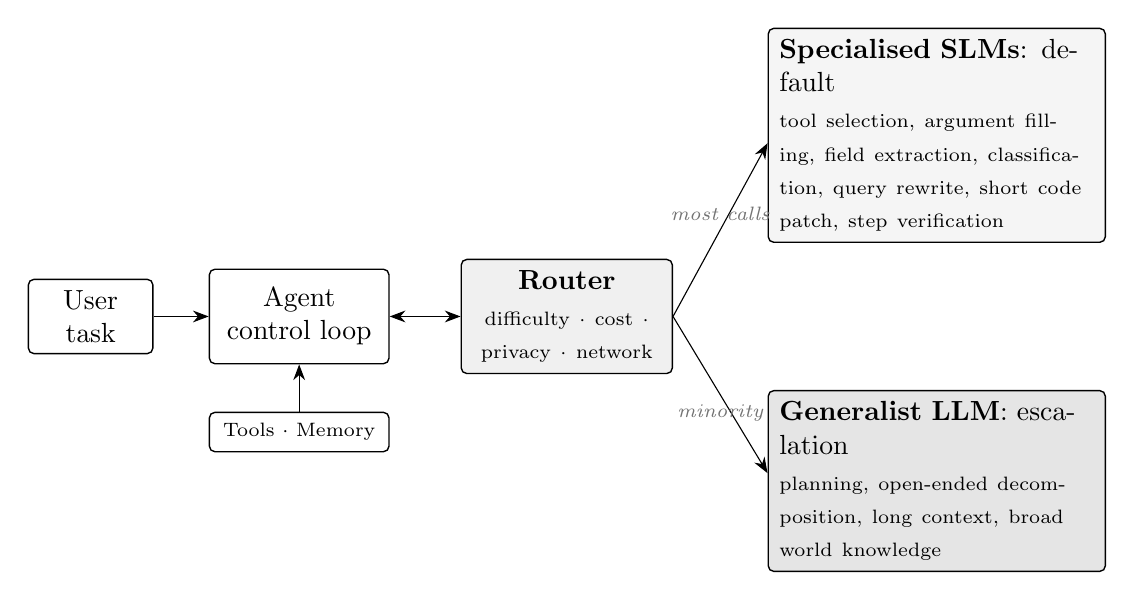
\begin{tikzpicture}[
  >={Stealth[length=2mm]},
  box/.style={draw, rounded corners=2pt, align=center, inner sep=4pt, line width=0.5pt},
  slm/.style={box, fill=black!4, text width=40mm, align=left},
  llm/.style={box, fill=black!10, text width=40mm, align=left},
  router/.style={box, fill=black!6, text width=24mm, minimum height=10mm},
  lbl/.style={font=\scriptsize\itshape, text=black!55},
]
\node[box, text width=13mm] (task) {User task};
\node[box, right=7mm of task, minimum height=12mm, text width=20mm] (loop) {Agent\\control loop};
\node[box, below=6mm of loop, font=\scriptsize, text width=20mm] (tools) {Tools $\cdot$ Memory};
\node[router, right=9mm of loop] (router) {\textbf{Router}\\[1pt]\scriptsize difficulty $\cdot$ cost $\cdot$ privacy $\cdot$ network};
\node[slm, above right=2mm and 12mm of router] (slm) {\textbf{Specialised SLMs}: default\\[1pt]\scriptsize tool selection, argument filling, field extraction, classification, query rewrite, short code patch, step verification};
\node[llm, below right=2mm and 12mm of router] (llm) {\textbf{Generalist LLM}: escalation\\[1pt]\scriptsize planning, open-ended decomposition, long context, broad world knowledge};
\draw[->] (task) -- (loop);
\draw[->] (tools) -- (loop);
\draw[<->] (loop) -- (router);
\draw[->] (router.east) -- ($(slm.west)+(0,-1mm)$) node[lbl, midway, above] {most calls};
\draw[->] (router.east) -- ($(llm.west)+(0,1mm)$) node[lbl, midway, below] {minority};
\end{tikzpicture}
\caption{Heterogeneous SLM--LLM agent. A per-call router sends the majority of
delegated sub-tasks to specialised small models and escalates only planning-like
or long-context calls to a generalist \gls{llm}; tools and memory are shared. After
\citet{belcak2025slm_agentic}.}
\Description{Block diagram of a heterogeneous agent. A user task feeds an agent control loop that shares tools and memory and consults a router. The router sends most calls to specialised small language models handling tool selection, argument filling, extraction, classification, query rewriting, short code patches, and step verification, and escalates a minority of calls to a generalist large language model for planning, open-ended decomposition, long context, and broad world knowledge.}
  \label{fig:hetero_agent}
\end{figure}

\subsubsection{Learned Routing}
\label{subsubsec:agentic_routing}

RouteLLM \citep{ong2024routellm} trains a lightweight router on human-preference data to predict, for each query, whether a weak model's answer would be judged as good as a strong model's, and dispatches accordingly; the authors report cost reductions of more than 2$\times$ on standard benchmarks with no measurable quality loss, and transfer of the trained router to unseen strong/weak model pairs. Division-of-Thoughts \citep{division_of_thoughts_2025} pushes routing below the query level, decomposing a task into sub-questions and assigning each to a local \gls{slm} or a cloud \gls{llm} according to estimated difficulty, for on-device agents. The open problems are difficulty estimation without an oracle, routing objectives that jointly weigh accuracy, latency, privacy sensitivity, and network availability, and handoff that does not produce a visible seam in output quality \citep{demystifying2025slm}.

\subsubsection{Production Instances}
\label{subsubsec:agentic_production}

Two large deployments already embody the heterogeneous pattern. Apple's Foundation Models framework pairs an on-device model of roughly 3B parameters, quantized with 2-bit quantization-aware training and KV-cache sharing, with a Private Cloud Compute server model built on a Parallel-Track Mixture-of-Experts transformer, and routes to the server only when the on-device model is expected to fall short \citep{gunter2025afm}. The on-device model is reported to be competitive with Qwen3-4B and Gemma-3-4B on its target tasks. Third-party providers can now register cloud models behind the same API surface as the local model, making the \gls{slm} the default and the \gls{llm} an opt-in escalation \citep{apple2026afm3}. Samsung's Gauss and Google's Gemini Nano occupy the same design point on their respective platforms \citep{samsung2023gauss}.

\subsection{Converting an LLM Agent to an SLM Agent}
\label{subsec:agentic_conversion}

For teams with an existing LLM-only agent, \citet{belcak2025slm_agentic} propose a six-step conversion pipeline that we summarize here because it operationalizes the position. \textbf{S1, instrumentation:} log every non-interface model call (inputs, outputs, latency) from the running agent, with encryption and access control. \textbf{S2, curation:} strip personally identifiable and protected health information and application secrets from the logs. \textbf{S3, clustering:} apply unsupervised clustering to the curated calls to surface the recurring request types, which are the specialization targets. \textbf{S4, selection:} for each cluster, choose a candidate \gls{slm} by matching required capability against benchmarks, license, and deployment constraints. \textbf{S5, specialization:} fine-tune the chosen \gls{slm} on the cluster's curated data, typically with \gls{lora} or \gls{qlora}. \textbf{S6, iteration:} re-run the loop periodically as the traffic distribution drifts. The pipeline is attractive precisely because the data it needs is a by-product of running the agent, and because each cluster converted removes a recurring frontier-model bill.

\subsection{Barriers to Adoption}
\label{subsec:agentic_barriers}

\citet{belcak2025slm_agentic} identify three reasons the shift has lagged the technical case. First, large centralized-inference investments create sunk-cost inertia and an operational bias toward one big model behind one API (B1). Second, \glspl{slm} are still evaluated on generalist leaderboards (\gls{mmlu}, broad chat benchmarks) that are misaligned with agentic utility, so their fitness for delegated sub-tasks is under-measured (B2). Section~\ref{sec:reported} shows the gap to be worse than a matter of emphasis: public reporting on these generalist benchmarks is itself too inconsistent to support cross-model comparison, so agentic fitness is not merely under-measured but currently unmeasurable from published sources. Third, \gls{slm} releases receive far less attention than frontier launches, so awareness lags capability (B3). The first and third are not technical obstacles and are eroding as routing frameworks mature and on-device platforms ship \glspl{slm} by default. The second is different, and Section~\ref{subsec:agentic_evidence} shows it to be partly a real evidential gap rather than only a misdirected one: agent-specific evaluation exists and is maturing \citep{patil2025bfcl,yao2024taubench,liu2024agentbench}, but it reports sub-10B models sparsely and reports cost per completed task essentially not at all. Until that changes, the strength of the case for hypothesis~H will remain uneven across its premises in the way Table~\ref{tab:agentic_evidence} records.

% ================================================================
% Section: Domain-Specific Applications
% From main (2).tex — Section VII
% ================================================================

\section{Domain-Specific Applications}
\label{sec:applications}

The domains below are where \gls{slm} deployment is most advanced, and each is an
agentic setting in the sense of Section~\ref{sec:agentic}: a workflow of bounded,
repeated language operations (extract a diagnosis code, classify a clause,
complete a function, translate a passage) executed under regulatory or cost
constraints that make a cloud frontier model impractical. Domain fine-tuning of a
small model is the LLM-to-SLM conversion pipeline
(\suppsec~\ref{subsec:agentic_conversion}) applied to a vertical.

\suppsec~\ref{supp:applications} reviews four verticals in detail, with the state of the evidence for each stated separately. In brief: healthcare is the best-evidenced vertical, with Meerkat-7B reporting 70.6\% on MedQA \citep{kim2025meerkat} and compressed clinical encoders losing under 5\% in macro-AUROC \citep{hasan2024optimclm}, but the case rests on exam benchmarks and single studies rather than on deployment evidence, and on-premises hosting removes one data-transfer question without by itself satisfying HIPAA or the GDPR. Legal \gls{nlp} has a strong structural case for small on-premises models and no independent capability evidence. Code has mature small models evaluated on public benchmarks \citep{roziere2023codellama,lozhkov2024starcoder2,zhu2024deepseek_coder}. Multilingual coverage trades breadth against depth at this size \citep{ustun2024aya,aryabumi2024aya23}. In every vertical the deployment interest runs ahead of the evidence.

\section{Discussion}
\label{section:discussion}

\subsection{What the Evidence Supports}
\label{subsec:discussion_key_findings}

Read together, the taxonomy (Section~\ref{sec:taxonomy}), the compression review
(Section~\ref{sec:compression}), and the audit of the evaluation record
(Section~\ref{sec:reported}) support four claims.

\textbf{Capability per parameter has risen sharply.} The strongest 3--4B models
of 2026 report scores on mathematics, code, and knowledge benchmarks that were
state of the art for 13B-class systems in 2023. Within families that publish
controlled ablations, the dominant explanatory variable is training data rather
than architecture: corpus composition and curation move results more than any
architectural choice available at this scale. The practical implication for model
builders is that data pipelines dominate architectural novelty as a lever on
\gls{slm} quality.

\textbf{Compression is a first-class capability, not an afterthought.} INT8 is
effectively lossless (\evB) and INT4 costs a small, non-uniform amount of
accuracy, with smaller models and mathematical reasoning at the higher end
(\evC). Because single-stream autoregressive decoding is memory-bandwidth-bound,
4-bit quantization is simultaneously a storage optimization and a decode-time
speedup on edge hardware, in proportion to the bandwidth it frees and subject to
the regime conditions of Section~\ref{subsec:deployment_calc_vs_meas}.
Quantization preserves fidelity better than pruning below 4B parameters
(\evB, \citealp{kurz2025pruning_vs_quant}), which simplifies the practitioner's
decision: quantize aggressively, and prune only when a structured size reduction
is independently required. What the literature does not support, and what
Section~\ref{subsec:compression_reporting} withdraws, is a single accuracy-retention
figure per technique: retention depends on baseline, model, size, task, and
aggregation rule, and a number stated without them is not interpretable.

\textbf{Right-sizing beats scaling for bounded tasks.} A quantized 3.8B model
that clears a task's accuracy threshold, running on hardware that already exists
in the user's hand, is preferable on cost, latency, energy, and data exposure to
a larger model that also clears it. A 3--4B model at INT4 occupies roughly 2~GB
and runs at interactive speed on a phone or a Jetson-class module. The
scaling-era assumption that a larger model is always the safer default is
inverted for any task whose requirements can be stated in advance \emph{and
checked}. Both halves of that condition matter: where the requirement cannot be
stated in advance, the task is not bounded, and where success cannot be checked,
per-call errors compound silently across an agent trajectory
(Section~\ref{subsubsec:agentic_ev_e2e}). Section~\ref{subsec:agentic_counterexamples}
lists the workload classes where this claim does not apply.

\textbf{The evaluation record is the weak point, and it is weaker than the field
acknowledges.} Section~\ref{sec:reported} documents why a cross-model accuracy
comparison cannot be built from current public reporting: benchmark sets do not
intersect across vendors, shot counts vary per benchmark and per vendor, base and
instruction-tuned figures are conflated, and matched baselines are rarely
published. This is not a limitation peculiar to this survey. It applies equally
to the comparison tables circulated in secondary sources, community leaderboards,
and prior surveys, which are widely reproduced without these caveats and which
practitioners use to make procurement decisions. Establishing a shared,
independently run evaluation for this model class would be a more valuable
contribution to the field than another survey, and
Section~\ref{subsec:challenges_verification} specifies what it would require.

\subsection{Implications for Agentic Systems}
\label{subsec:discussion_agentic}

The agentic argument of Section~\ref{sec:agentic} rests on these claims rather
than restating them. Capability-per-parameter growth is what makes an \gls{slm}
\emph{sufficient} for a delegated sub-task; compression and edge deployability are
what make it \emph{cheap} and \emph{private}; right-sizing is the design
discipline that turns a heterogeneous SLM--LLM system from an option into the
default. Two cross-cutting observations sharpen the picture. First, routing must
be capability-aware, not size-aware: the reported multilingual and safety gaps
(Section~\ref{subsec:reported_safety}) mean that a naive ``small model unless
hard'' router will silently degrade non-English and safety-sensitive calls.
Second, adaptation matters more as models get smaller, so the economical unit in
an agent is often a \emph{fine-tuned} small model per recurring call type rather
than a single general \gls{slm}, which is exactly what the LLM-to-SLM conversion
pipeline of Section~\ref{subsec:agentic_conversion} produces.

\subsection{Democratization and Sustainability}
\label{subsec:discussion_implications}

Deploying a 3B model that answers grade-school mathematics correctly on an
\$80 single-board computer is a qualitative change in access. Organizations facing
cloud-API cost, data-sovereignty rules, or unreliable connectivity can now run
capable \gls{nlp} locally with no per-query charge and, subject to the scope
conditions of Section~\ref{subsec:deployment_privacy_scope}, without transferring
prompt content to a processor outside their control.

The environmental case is narrower than it is usually stated and we state it
narrowly. Reported per-inference energy for a small model on modest hardware is
one to two orders of magnitude below a frontier-model query in a datacenter, so
for a task the small model completes correctly, serving it small uses
substantially less inference energy. Whether a wholesale shift reduces total
system energy is a different question, and one no published accounting answers:
it turns on teacher-training energy, the compression pipeline, device embodied
carbon, regional grid intensity, update distribution, and the rebound effect, none
of which the available reporting covers.
Section~\ref{subsubsec:challenges_env_scope} sets out that accounting boundary in
full. We therefore make the per-query claim and decline the aggregate one.

\subsection{Limitations}
\label{subsec:discussion_limitations}

Beyond the evidence-base limitations already stated
(Section~\ref{subsec:reported_limits}), six bound this work.

\emph{No original measurement.} No benchmark was executed for this survey. Every
quantitative claim is therefore at best grade~\evB{}
(Section~\ref{subsec:reported_grading}), and the paper contains no grade~\evA{}
evidence. This is a deliberate choice, since we judged an audit of the record more
useful than adding another unreplicated table to it, but it is a limitation and
Section~\ref{subsec:challenges_verification} is written to be acted on rather than
cited.

\emph{The definitional boundaries are conventions.} The twenty-billion threshold,
the split into conditions C1 and C2, and the sub-10B restriction on the evaluation
cohort are pragmatic choices, not natural kinds. They are stated precisely
(Section~\ref{subsec:intro_definition}) so that a reader can recompute under
different ones, which is the most a threshold of this sort can offer.

\emph{The thesis is a hypothesis.} The agentic argument is grounded in a
production-scale position paper \citep{belcak2025slm_agentic}, two large
deployments, and the agent-specific evidence of
Section~\ref{subsec:agentic_evidence}, and its premises are graded individually in
Table~\ref{tab:agentic_evidence}. The end-to-end claim, that a small-model agent
completes realistic tasks at comparable rate and lower cost per completed task,
is the one premise for which we found no evidence either way. It is a projection,
and we mark it as one.

\emph{Coverage is English-centric.} The task coverage, the benchmarks audited, and
most of the compression literature are English-centric, which matters more here
than usual because compression degrades non-English performance disproportionately
(Section~\ref{subsec:discussion_ethics}).

\emph{Domain sections are uneven.} Code and healthcare have public benchmarks and
are treated evidentially; legal has neither, and
Section~\ref{subsec:applications_legal} states a structural argument rather than a
capability claim. Readers should not read the four verticals as equally supported.

\emph{The snapshot ages.} The ecosystem moves faster than a review cycle. The
update policy of Section~\ref{subsubsec:intro_snapshot} and the versioned deposit
are how we bound this, not eliminate it.

\subsection{Ethical Considerations}
\label{subsec:discussion_ethics}

Safety alignment is proportionally harder at small scale: several research-grade
\glspl{slm} lack the safety training of their larger siblings, and fine-tuning can erode
what alignment exists \citep{qi2023finetuning}. Practitioners deploying SLMs, and
especially those wiring them into agents with tool access, should treat
application-level safety filtering and output monitoring as mandatory, not
optional. Compression carries its own risk: pruning and quantization can degrade
performance unevenly across dialects, languages, and demographic groups
\citep{blodgett2020language}, and the reported advantage of quantization over
pruning is largest precisely on multilingual tasks \citep{kurz2025pruning_vs_quant},
which suggests pruning disproportionately harms non-English users. Fairness-aware
compression objectives and per-group performance floors for high-stakes
applications are open requirements. Against these risks, on-device \glspl{slm} advance
privacy (one egress channel removed, subject to Section~\ref{subsec:deployment_privacy_scope}), accessibility (no connectivity required),
and cost (no subscription), which matters most for the healthcare and
educational applications of Section~\ref{sec:applications} in under-resourced
settings.

% ================================================================
% Section: Challenges and Future Directions
% From main (2).tex — Section VIII + sections/conclusion.tex future work
% ================================================================

\section{Challenges and Future Directions}
\label{sec:challenges}

Despite remarkable progress, \glspl{slm} face persistent challenges that define the frontier of the field, and the agentic framing of Section~\ref{sec:agentic} adds a set of its own. We organize these into research clusters, closing with the empirical-verification agenda for this paper's consolidated evidence base.

\subsection{Hallucination Mitigation in Small Models}
\label{subsec:challenges_hallucination}

Hallucination, the confident generation of factually incorrect content, is an intrinsic failure mode of autoregressive language models, and it is more pronounced in smaller models \citep{zhang2023siren}. The core issue is information capacity: a 3B model's parameters can encode far fewer facts than a 175B model, and when queried about knowledge at the boundary of its training distribution, small models are more likely to confabulate plausible-sounding but incorrect responses.

Mitigation strategies include: (1)~\emph{\gls{rag}} \citep{lewis2020rag}, which anchors \gls{slm} generation to retrieved documents rather than parametric memory; (2)~\emph{uncertainty quantification} through sampling and ensemble methods; (3)~\emph{RLHF with truthfulness rewards} to penalize confident incorrect responses; and (4)~\emph{calibration post-processing} to align model confidence to actual accuracy.

\subsection{Reasoning Limitations Under Parameter Constraints}
\label{subsec:challenges_reasoning}

Complex multi-step reasoning, particularly in mathematics, formal logic, and scientific inference, improves roughly as a power law with parameter count \citep{kaplan2020scaling}. At the 1B--7B scale, \glspl{slm} struggle with problems that require holding many intermediate states simultaneously or with deep deductive chains.

Emerging directions include: (1)~\emph{Test-time scaling}: allocating additional inference compute (more generation tokens, repeated sampling, tree-of-thought search) to substitute for model capacity; DeepSeek-R1 \citep{deepseek2025r1} achieves frontier-class reasoning in its 7B distilled variant through extended chain-of-thought generation. (2)~\emph{Neuro-symbolic integration}: augmenting \glspl{slm} with symbolic solvers (SAT solvers, theorem provers, calculators) to handle formal reasoning externally. (3)~\emph{Speculative decoding} \citep{leviathan2023speculative} using a small draft \gls{slm} to propose tokens verified by a larger model, enabling faster inference from larger models when latency permits.

\subsection{Open Problems for Agentic SLM Systems}
\label{subsec:challenges_routing}

Section~\ref{sec:agentic} argues that \glspl{slm} are the appropriate default substrate for the class of agent calls hypothesis~H names; several problems stand between that conditional position and routine practice. \textbf{Difficulty estimation without an oracle:} a router must decide, cheaply and before generation, whether a given call exceeds the local model's competence; current approaches use learned win-prediction \citep{ong2024routellm} or sub-task decomposition \citep{division_of_thoughts_2025}, but calibration under distribution shift is unsolved. \textbf{Multi-objective routing:} the decision must jointly weigh accuracy, latency, energy, monetary cost, privacy sensitivity, and network availability, and the reported multilingual and safety gaps (Section~\ref{subsec:reported_safety}) mean a size-only router silently degrades non-English and safety-critical calls. \textbf{Handoff without a seam:} escalation from \gls{slm} to \gls{llm} mid-task must not produce a visible discontinuity in style or quality. \textbf{Agent-appropriate evaluation:} generalist leaderboards do not measure the tool-selection, argument-filling, and format-adherence skills agents actually use \citep{belcak2025slm_agentic}; function-calling leaderboards \citep{patil2025bfcl,zhang2024xlam} and interaction benchmarks \citep{yao2024taubench} are a start, but they report sub-10B models sparsely, and none reports cost per completed task (Section~\ref{subsubsec:agentic_ev_routing}). \textbf{Fleet management:} an agent built from many fine-tuned sub-3B specialists (Section~\ref{subsec:agentic_conversion}) raises questions of versioning, drift detection, and retraining cadence that single-model deployments do not face. Apple's privacy-preserving cloud escalation \citep{apple2024intelligence,gunter2025afm} shows the pattern is production-viable; generalizing it beyond a single vendor's stack is open.

\subsection{Hardware Co-Design and NPU Optimization}
\label{subsec:challenges_hardware}

The efficiency of \gls{slm} inference depends as much on hardware as on model architecture. Modern consumer hardware increasingly includes dedicated AI accelerators: Apple ANE, Qualcomm Hexagon \gls{npu} \citep{qualcomm2024ondevice}, Samsung Exynos \gls{npu}, and Intel \gls{npu}. These accelerators are optimized for specific operation types (INT4/INT8 matrix multiplication) and data layouts.

A critical open problem is \emph{hardware-model co-design}: developing \gls{slm} architectures whose attention patterns, FFN widths, and layer counts align with the data bus widths and tile sizes of target \glspl{npu}. \gls{gqa} head counts of 8 or 16 align well with SIMD widths on ARM Cortex-A processors, while head counts of 32 may be suboptimal. Future \glspl{slm} trained with hardware constraints as first-class objectives, rather than retrofitting quantization after the fact, will likely yield significant efficiency improvements.

\subsection{Ethical Considerations: Bias Amplification in Compressed Models}
\label{subsec:challenges_ethics}

Model compression introduces an underexplored ethical risk: \emph{bias amplification}. Pruning and quantization may disproportionately affect model performance on underrepresented demographic groups, dialects, and languages, as the model's remaining capacity may preferentially serve the majority distributions present in training data \citep{blodgett2020language}. \citet{kurz2025pruning_vs_quant} observe that quantization's advantage over pruning is most pronounced for multilingual tasks, suggesting that pruning disproportionately degrades non-English performance.

Research priorities include: (1)~\emph{fairness-aware compression} that includes demographic parity metrics as part of the compression objective; (2)~\emph{representation auditing} of compressed models across language, dialect, gender, and race; and (3)~\emph{minimum performance floors} for safety-critical applications, ensuring compressed models meet baseline accuracy thresholds for all user populations.

\subsection{Sustainable AI: SLMs as a Green AI Alternative}
\label{subsec:challenges_sustainability}

The energy consumption of training and serving frontier \glspl{llm} has become a significant environmental and economic concern \citep{strubell2019energy,patterson2022carbon}. Training GPT-3 emitted an estimated 552 metric tons of CO$_2$ equivalent \citep{patterson2021carbon}; training a model two orders of magnitude smaller from scratch consumes correspondingly less, and per-query inference energy is lower in proportion to the compute each query performs.

\subsubsection{What the Environmental Claim Covers}
\label{subsubsec:challenges_env_scope}

Claims of this kind are routinely made at a level of generality the accounting
does not support, and we withdraw one we made in an earlier draft. The statement
that 10,000 concurrent small-model instances on consumer hardware consume less
total energy than a single multi-GPU server is not one we can source or derive:
its truth depends entirely on utilization on both sides, and a server at high
batch utilization is considerably more energy-efficient per token than an idle
consumer device performing occasional single-stream inference. We remove the
claim rather than qualify it.

What can be said requires the boundary of the accounting to be stated. A complete
comparison of a small-model deployment against a large-model one has to include:
the training energy of the small model itself; the training energy of any
\emph{teacher} used to distill it, which for a distilled model can dominate and
which vendors do not report; the energy of the distillation, quantization, or
pruning pipeline that produced the deployed artifact; the embodied carbon of
manufacturing the devices inference runs on, amortized over their service life
and over the share of that life spent on inference; the marginal grid intensity
where each side runs, which differs by more than a factor of ten between regions;
and the energy of model updates over the deployment's lifetime, which for
on-device models means redistributing weights to every device rather than
updating one server.

Almost none of these terms is reported in the literature. What the field has
instead is per-query inference energy on the two sides, which is a single term in
a much longer sum, and which does favor the small model by one to two orders of
magnitude for a query both can answer. The defensible claim is therefore narrow:
\emph{for a task a small model completes correctly, serving it with the small
model uses substantially less inference energy}. Whether a wholesale shift to
small models reduces total system energy is a question no published accounting
answers, and the rebound effect, that cheaper inference induces more of it, cuts
against it. As AI regulation incorporates carbon disclosure requirements, this
accounting will have to be done properly, and the inputs for it do not currently
exist.

\subsection{Empirical-Verification Opportunities}
\label{subsec:challenges_verification}

Because this review synthesizes reported performance rather than producing original benchmark runs, the most immediately valuable follow-up work is targeted empirical verification of the reported claims that do the most work in practitioner decisions. Four empirical studies would disproportionately reduce the residual uncertainty in the evidence base reviewed here:

\begin{description}
    \item[Harness-consistent reruns of the headline \glspl{slm} on the headline benchmarks] A controlled re-run of the seven most-cited \glspl{slm} (Phi-4-mini, Phi-4, Qwen2.5-3B, Qwen2.5-7B, Gemma-3-4B, Llama 3.2-3B, Mistral-7B) on \gls{mmlu}, \gls{gsm8k}, HumanEval, and MBPP under a single \texttt{lm-evaluation-harness} configuration would anchor every vendor-reported figure to an independent reproduction.
    \item[Quantization-degradation measurement] A controlled comparison of FP16 vs.\ INT8 vs.\ INT4 accuracy across the seven headline \glspl{slm} and four benchmarks, using the \gls{gguf}, GPTQ, and \gls{awq} toolchains referenced in the vendor reports, would sharpen the 1--4-point degradation figure reported in the literature.
    \item[Edge-throughput reproduction] Timed runs of the same seven \glspl{slm} in their best-supported INT4 format on a Raspberry~Pi~5, Jetson Orin Nano, Snapdragon reference device, and recent laptop CPU would calibrate the reported throughput ranges against modern silicon.
    \item[QLoRA-gain reproduction] A controlled \gls{qlora} (rank 64, $\alpha = 128$) adaptation of the seven \glspl{slm} on SST-2, MNLI, ARC-C, \gls{gsm8k}, and SQuAD~2.0 would quantify the reported fine-tuning gains under a single adaptation recipe.

    \item[Cost per completed task, small-model against large-model agent] The measurement this survey most needs and could not find (Section~\ref{subsubsec:agentic_ev_routing}). Fix one agentic workload with a checkable success criterion, for instance a $\tau$-bench domain \citep{yao2024taubench} or a WebArena subset \citep{zhou2024webarena}. Run three configurations end to end: a frontier model throughout; a specialized \gls{slm} throughout; and a routed heterogeneous system. Report, per configuration, end-to-end task success, the number of model calls per completed task including retries, escalation rate, wall-clock latency, and total monetary and energy cost per \emph{completed} task rather than per call. This single study would move the economic premise of hypothesis~H from grade~\evC{} to grade~\evA{}, and it would settle whether per-token savings survive the retry and escalation overhead that per-call accounting hides.

    \item[Agent-specific evaluation of the sub-10B cohort] Run the seven headline \glspl{slm} on the Berkeley Function-Calling Leaderboard \citep{patil2025bfcl} and on $\tau$-bench, reporting the pass\textsuperscript{$k$} consistency metric alongside single-attempt accuracy, with and without constrained decoding \citep{willard2023guided}. This would fill the sparse-coverage gap identified in Table~\ref{tab:agentic_evidence} and would separate well-formedness failures from content failures, which current reporting conflates.
\end{description}

The first four studies are practical on a single modern GPU on the time scale of weeks. The last two require an agent harness and a modest API budget but no unusual resources, and they are the two that bear on the paper's central hypothesis rather than on its survey material. Together they would convert several consolidated claims from ``reported by sources'' to ``empirically verified,'' and would supply the first grade-\evA{} evidence in an area that currently has none. They do not replace the review; they strengthen the claims that practitioners depend on most.

\subsection{Open Research Directions Beyond Empirical Verification}
\label{subsec:challenges_future}

Beyond direct empirical verification, several promising research directions emerge from this review:

\begin{description}
    \item[Multilingual \gls{slm} evaluation] Extending the consolidated performance evidence to non-English benchmarks would reveal whether the English-centric performance hierarchy reported in the literature holds across languages, particularly for models with multilingual training data (Qwen2.5, Gemma~3, BLOOM).

    \item[On-device continual learning] Developing methods for incremental adaptation of deployed \glspl{slm} to new data without full retraining would enable personalization and domain adaptation at the edge.

    \item[SLM ensembles vs.\ single \gls{llm}] Investigating whether ensembles of specialized \glspl{slm} (one for math, one for code, one for general knowledge) with a lightweight router can match single-LLM performance at lower aggregate cost.

    \item[Multimodal \glspl{slm}] Evaluating vision-language \glspl{slm} such as Phi-3-vision, Gemma~3 with vision, and Gemma~3n \citep{google2025gemma3n} on multimodal benchmarks would extend the comparison to the rapidly growing multimodal inference domain.

    \item[Hybrid architectures] The emergence of non-transformer \gls{slm} architectures (SambaY \citep{pal2025sambay}, Gated Delta Networks \citep{yang2025gated_delta}) suggests that the transformer's dominance may not extend to the edge, where linear-time inference is particularly valuable.

    \item[Federated fine-tuning] Developing privacy-preserving fine-tuning protocols that aggregate gradient updates across edge devices would enable collaborative model improvement without centralized data collection.
\end{description}

\section{Conclusion}
\label{section:conclusion}

This survey fixed a two-condition definition that separates a model's per-token cost from its storage cost, cataloged 179 \glspl{slm} and, separately, 30 small-active-parameter mixtures of experts released from 2023 to September 2026 with every record's developer source checked, reviewed compression along separate axes, and quantified why the vendor evaluation record cannot support cross-model comparison: for the 14 cohort models of the four largest vendors, no benchmark is reported for all of them and no stated protocol is shared by more than five. Single-harness third-party evaluations, not vendor tables, are the basis on which comparison should rest.

On the agentic question, we stated the case for small models as a conditional hypothesis. For call types that are bounded, recurrent enough to clear a break-even volume that counts retries, checks, and escalations, short-context, and checkable for correctness as well as validity, a specialized small model should be the default, with escalation to a frontier model when a check fails. The evidence supports this unevenly. Developers report specialized sub-10B models competitive on single- and multi-turn function calling, while independent work shows that off-the-shelf small models often are not; end-to-end comparisons are contested; cost per correct answer has been measured for single-turn tasks and frontier agents; and no study measures cost per completed task for a small-model-first agent against the alternatives, including cached, batched, and fine-tuned hosted models. Where the conditions fail, for planning, long-context synthesis, and uncheckable work, a frontier model remains the right choice.

The pre-registered comparison of Section~\ref{subsec:challenges_verification}, with its comparators, decision rule, and sample size, is the shortest route from what has been reported to what has been established. Until it is run, the position defended here is a design hypothesis with a stated domain: specialized small models doing the bounded, recurrent, checkable work, and a large model for planning, synthesis, and the calls no cheap check can verify.

\section*{Declarations}
\addcontentsline{toc}{section}{Declarations}

% -----------------------------------------------------------------------------
% AUTHOR ACTION REQUIRED: replace the bracketed placeholders before submission.
% Springer Nature also requires the Competing Interests and Author Contributions
% statements to be entered into Editorial Manager separately.
% -----------------------------------------------------------------------------

\subsection*{Funding}
% e.g. "This work was supported by [funder] under grant [number]."
[No funding was received for this work.]

\subsection*{Competing interests}
The authors declare that they have no competing interests.
% Replace if any author has a financial or non-financial competing interest.

\subsection*{Ethics approval and consent to participate}
Not applicable. This study is a literature review and analysis of publicly
available model documentation; it involves no human participants, human data, or
animals.

\subsection*{Consent for publication}
Not applicable.

\subsection*{Data availability}
This paper is a review. All performance figures are \emph{reported} values
compiled from public sources---vendor technical reports, official model cards,
community leaderboards, and third-party evaluations---and are not the product of
original benchmark runs. Every consolidated figure is traced to a dated, citable
source in Appendix~\ref{app:provenance}. The model-ecosystem inventory analysed in
Section~\ref{sec:taxonomy} and Appendix~\ref{appendix:ecosystem} is generated from
the dataset \texttt{merged\_llm\_database.json} (snapshot September~2026), provided
with the manuscript source files.

\subsection*{Code availability}
The scripts that generate the ecosystem inventory tables and the figures
(\texttt{generate\_model\_tables.py}, \texttt{generate\_figures\_v2.py}) are
provided with the manuscript source files. No model-training or model-evaluation
code was used to produce the results in this paper, which are compiled from the
published literature.

\subsection*{Author contributions}
% CRediT taxonomy --- edit to reflect actual contributions.
\textbf{M.G.R.:} Conceptualization, Methodology, Investigation, Data curation,
Software, Writing --- original draft, Visualization.
\textbf{H.A.:} Conceptualization, Methodology, Writing --- review \& editing,
Supervision, Project administration.
\textbf{S.J.A.:} Investigation, Validation, Writing --- review \& editing.
\textbf{A.A.:} Validation, Writing --- review \& editing, Funding acquisition.
All authors read and approved the final manuscript.

\subsection*{Acknowledgements}
% Acknowledge non-author contributions, facilities, and technical assistance, or delete.
[The authors thank \dots{} .]


\bibliographystyle{ACM-Reference-Format}
\bibliography{bibliography}

\appendix
\section{Data Provenance and Supplementary Protocols}
\label{appendix:supplementary}
\label{app:provenance}

This appendix supports the reproducibility of the \emph{review itself}: it documents the sources of the reported figures consolidated in Sections~\ref{sec:reported}--\ref{sec:deployment}, and provides the reference prompt templates and quantization-pipeline specifications under which those figures were reported. (The \gls{qlora} adaptation recipe appears in Section~\ref{sec:reported}, Table~\ref{tab:hyperparam_search}; detailed device specifications appear in Section~\ref{sec:deployment}, Table~\ref{tab:appendix_hardware}.) The appendix does not report original experimental runs.

\subsection{Provenance of the Consolidated Figures}
\label{subsec:appendix_provenance_table}

% -----------------------------------------------------------------------------
% AUTHOR ACTION REQUIRED BEFORE SUBMISSION.
% Table \ref{tab:provenance_models} below records model-level provenance, which is
% complete. Per-cell attribution for Tables \ref{tab:finetuning},
% \ref{tab:edge_deployment}, \ref{tab:energy} and \ref{tab:latency_compare} is NOT
% yet reproduced anywhere in this manuscript. Either (a) supply the per-cell
% source ledger for those four tables, or (b) withdraw them and the claims that
% depend on them. Section \ref{subsec:appendix_provenance_status} states the
% current position honestly, but it is not a substitute for (a) or (b).
% -----------------------------------------------------------------------------

Provenance is recorded at two levels. \emph{Model-level} provenance fixes, for
each model in the cohort, the primary release document from which its
architectural specification and headline benchmark scores derive
(Table~\ref{tab:provenance_models}). \emph{Source-class} provenance records, for
each consolidated table, the categories of source the figures are drawn from and
the reconciliation rules applied
(Section~\ref{subsec:appendix_provenance_status}). Benchmark definitions and
metric variants follow the originating task papers cited in
Section~\ref{subsec:reported_benchmarks}.

\begin{table}[ht]
\centering
\caption{Model-level provenance for the reviewed cohort: the primary release document from which each model's architectural specification and headline reported scores derive.}
\label{tab:provenance_models}
\footnotesize\adjustbox{max width=\linewidth}{%
\begin{tabular}{llll}
\toprule
\textbf{Model(s)} & \textbf{Developer} & \textbf{Primary source} & \textbf{Source type} \\
\midrule
TinyLlama-1.1B & --- & \citet{zhang2024tinyllama} & Technical report \\
SmolLM2-1.7B, -360M & Hugging Face & \citet{allal2025smollm2} & Technical report \\
StableLM 2-1.6B & Stability AI & \citet{stabilityai2024stablelm} & Technical report \\
Qwen2.5-0.5B/1.5B/3B/7B & Alibaba & \citet{qwen2024qwen25} & Technical report \\
Llama 3.2-1B/3B & Meta & \citet{grattafiori2024llama3} & Technical report \\
Gemma 2-2B/9B & Google DeepMind & \citet{gemma2team2024} & Technical report \\
Gemma 3-1B/4B & Google DeepMind & \citet{team2025gemma3} & Technical report \\
Mistral 7B & Mistral AI & \citet{jiang2023mistral} & Technical report \\
Phi-3-mini & Microsoft & \citet{abdin2024phi3} & Technical report \\
Phi-3.5-mini & Microsoft & \citet{abdin2024phi35} & Technical report \\
Phi-4-mini & Microsoft & \citet{microsoft2025phi4mini} & Technical report \\
Phi-4 & Microsoft & \citet{abdin2024phi4} & Technical report \\
Ministral 8B & Mistral AI & Vendor model card & Model card \\
\bottomrule
\end{tabular}%
}
\end{table}

\subsection{Provenance Status by Table}
\label{subsec:appendix_provenance_status}

The consolidated tables do not all rest on an equally firm reporting base, and
the distinction matters for how much weight each should carry.

\emph{Architectural and accuracy figures.} The specifications in
Table~\ref{tab:model_specs} and the accuracy figures in
Tables~\ref{tab:zero_shot} and~\ref{tab:appendix_zero_shot_extended} derive from
the primary release documents in Table~\ref{tab:provenance_models}, supplemented
where a model's report omits a task by standardized community evaluations
(the Open \gls{llm} Leaderboard and \texttt{lm-evaluation-harness}-based reports
\citep{gao2023harness}). These are the best-supported figures in the review.

\emph{Compression and quantization figures.} The degradation figures in
Table~\ref{tab:quantization} and the footprints in
Table~\ref{tab:memory_footprint} derive from the quantization-method literature
\citep{frantar2023gptq,lin2024awq,kim2024squeezellm} and from published
quantized artifact sizes. The comparative characteristics in
Table~\ref{tab:compression_compare} are a synthesis of the compression
literature reviewed in Section~\ref{sec:compression} rather than measurements of
a single cohort, and the retention column should be read as an indicative band
rather than a measured quantity.

\emph{Adaptation, efficiency, and energy figures.} Tables~\ref{tab:finetuning},
\ref{tab:edge_deployment}, \ref{tab:energy} and~\ref{tab:latency_compare} rest on
a materially thinner base. Public reporting of fine-tuning gains, edge
throughput, and per-inference energy is sparse, is rarely produced under a common
protocol, and in several cases exists only for a subset of the cohort; some
entries are consequently aggregates or interpolations across sources rather than
single quoted values, and this manuscript does not reproduce a per-cell ledger
for them. They are offered as indicative orders of magnitude that establish
relative position, not as measurements, and no claim in this paper should be
read as resting on their precise values. Converting them into measured
quantities is the first item on the verification agenda of
Section~\ref{subsec:challenges_verification}.

The remaining subsections of this appendix document the reference conditions---prompt formats, quantization toolchains, adaptation hyperparameters---that the reviewed sources most commonly report; these are preserved here so that readers can interpret any individual reported figure against the conditions it was measured under.

\subsection{Prompt Formats}
\label{subsec:appendix_prompt_templates}
The reviewed source materials commonly preserve each model's own instruction
wrapper while following a shared task-payload structure, which is summarized here
in prose. \textbf{Multiple-choice question answering} presents the question
followed by the enumerated options (A--D) and an ``Answer:'' cue, with the model
expected to emit a single option letter. \textbf{Mathematical reasoning} prepends
an instruction to solve the problem step by step and appends a ``Let's think step
by step'' cue, so that a chain-of-thought precedes the final numeric answer.
\textbf{Extractive question answering} supplies the context passage, then the
question, then an instruction to answer from the context and to respond
``unanswerable'' when the context does not contain the answer. \textbf{Abstractive
summarization} supplies the source article preceded by an instruction to produce a
two- to three-sentence summary. Where a source reports few-shot results, the same
fixed set of exemplars is prepended to the payload for every model on a given
task. Because sources differ in the exact wording of these wrappers and in
answer-extraction heuristics, the consolidated figures are compared only within
tasks and, wherever possible, within a single reporting source.

\subsection{Quantization and Compression Pipeline}
\label{subsec:appendix_quantization_pipeline}
To complement the methodology section, the compression workflows reported across the reviewed sources are summarized here. The reviewed literature reports five precision or compression settings across the consolidated comparison:
\begin{description}
    \item[FP16 baseline] Standard half-precision inference used as the reference condition.
    \item[GGUF Q4\_K\_M] Mixed-precision 4-bit quantization via \texttt{llama.cpp}, assigning higher precision to the most sensitive tensors.
    \item[AWQ 4-bit] Activation-aware weight quantization with group size 128 and calibration on held-out text sequences.
    \item[GPTQ 4-bit] Layer-wise post-training quantization using second-order curvature approximations.
    \item[bitsandbytes NF4] 4-bit NormalFloat quantization with double quantization, matching the \gls{qlora} training regime.
\end{description}

For compression stress tests, the sources report SparseGPT~\citep{frantar2023sparsegpt}-induced 50\% unstructured sparsity applied before 4-bit quantization. Reported figures for this combined pruning-plus-quantization setting are retained in the provenance tables for sensitivity analysis rather than the main comparative tables, because support for sparse inference remains hardware dependent and is not uniformly reported across the reviewed sources.

\subsection{Edge Measurement Protocols Reported in the Source Literature}
\label{subsec:appendix_edge_protocol}
The deployment figures consolidated in Sections~\ref{sec:reported}--\ref{sec:deployment} are drawn from source materials whose stated measurement protocols typically include a multi-minute warm-up to stabilize thermal and frequency behavior before measurement. Across the reviewed edge-deployment sources, the reported per-model, per-device measurements cover:
\begin{description}
    \item[Time-to-first-token (\gls{ttft})] Reported latency from prompt submission to first generated token, typically averaged over 50 prompts with 128-token inputs.
    \item[Sustained throughput] Reported mean tokens-per-second over 256-token generations.
    \item[Peak memory] Reported maximum RAM or unified-memory consumption during generation.
    \item[Load time] Reported elapsed time from process start until the model is ready to serve requests.
    \item[Energy per inference] Reported device-level power estimates where the source provides counter- or telemetry-based measurements.
\end{description}
Because these reporting conventions differ in small but potentially consequential ways across sources (warm-up duration, prompt-length distribution, power-counter granularity), readers should treat the consolidated figures as indicative rather than precisely comparable; the conflict-resolution rules in Section~\ref{subsec:reported_sources} are applied whenever discrepant protocols yield materially different reported values for the same tuple.

\subsection{Extended Results Tables}
\label{subsec:appendix_extended_results}
The representative five-shot results for the four models with fine-tuning
comparisons, and the QLoRA hyperparameter configuration used to produce them, are
given with the fine-tuning comparison itself in Section~\ref{sec:reported}
(Table~\ref{tab:finetuning}, Table~\ref{tab:hyperparam_search}) rather than
repeated here.

\begin{landscape}
\begin{table}[ht]
\centering
\caption{Extended zero-shot results across a broader task set (FP16, instruction-tuned variants). All values are reported figures.}
\label{tab:appendix_zero_shot_extended}
\footnotesize\adjustbox{max width=\linewidth}{%
\begin{tabular}{lcccccccccccc}
\toprule
\textbf{Model} & \textbf{ARC-E} & \textbf{ARC-C} & \textbf{HellaSwag} & \textbf{TriviaQA} & \textbf{SQuAD 2.0} & \textbf{GSM8K} & \textbf{MATH} & \textbf{HumanEval} & \textbf{MBPP} & \textbf{MMLU} & \textbf{SST-2} & \textbf{MNLI} \\
\midrule
Phi-4-mini-Inst. & 92.1 & 83.7 & 69.1 & 68.5 & 74.2 & 88.6 & 64.0 & 72.0 & 74.8 & 67.3 & 92.4 & 72.1 \\
Qwen2.5-7B-Inst. & 94.8 & 90.1 & 80.0 & 72.4 & 76.8 & 88.7 & 60.4 & 84.8 & 79.2 & 72.6 & 93.8 & 74.6 \\
Gemma 2-9B-Inst. & 95.2 & 89.8 & 87.1 & 71.8 & 75.5 & 84.9 & 51.3 & 68.9 & 73.5 & 71.3 & 93.5 & 73.8 \\
Gemma 3-4B-Inst. & 92.4 & 85.2 & 78.4 & 64.2 & 70.8 & 82.1 & 53.7 & 64.6 & 69.3 & 65.8 & 91.2 & 70.4 \\
LLaMA 3.2-3B-Inst. & 88.5 & 76.1 & 77.2 & 58.6 & 65.4 & 75.6 & 46.7 & 58.5 & 62.4 & 61.8 & 88.2 & 63.5 \\
LLaMA 3.2-1B-Inst. & 78.2 & 62.3 & 63.8 & 42.5 & 52.8 & 47.2 & 24.1 & 35.4 & 40.2 & 48.6 & 82.5 & 54.2 \\
Mistral 7B-Inst. v0.3 & 91.8 & 82.7 & 73.5 & 65.8 & 68.4 & 81.9 & 41.6 & 66.5 & 68.3 & 63.0 & 90.8 & 68.2 \\
Ministral 8B-Inst. & 93.2 & 85.4 & 76.8 & 67.2 & 71.2 & 83.5 & 45.2 & 69.5 & 71.8 & 65.7 & 92.1 & 71.5 \\
Qwen2.5-3B-Inst. & 90.2 & 78.6 & 72.1 & 58.8 & 66.5 & 79.8 & 50.2 & 65.2 & 67.8 & 65.6 & 89.5 & 66.8 \\
Qwen2.5-0.5B-Inst. & 68.4 & 52.1 & 48.3 & 28.5 & 38.2 & 38.5 & 18.7 & 22.0 & 28.4 & 47.5 & 78.2 & 48.5 \\
SmolLM2-1.7B-Inst. & 74.5 & 59.8 & 60.2 & 35.4 & 52.3 & 42.6 & 19.3 & 28.7 & 35.6 & 50.1 & 82.6 & 54.2 \\
SmolLM2-360M-Inst. & 55.8 & 38.2 & 42.5 & 18.2 & 32.4 & 15.8 & 5.2 & 8.5 & 12.3 & 33.4 & 72.4 & 42.8 \\
TinyLlama 1.1B & 62.4 & 47.5 & 53.8 & 28.8 & 42.5 & 18.4 & 6.8 & 12.2 & 16.8 & 36.2 & 76.5 & 46.2 \\
StableLM 2 1.6B & 72.8 & 55.2 & 57.6 & 32.5 & 48.6 & 32.1 & 12.4 & 22.5 & 28.9 & 44.3 & 80.2 & 52.5 \\
\bottomrule
\end{tabular}%
}
\end{table}
\end{landscape}

\subsection{Human-Evaluation Conventions in the Source Literature}
\label{subsec:appendix_human_eval}
For subjective tasks such as summarization quality and instruction following, the reviewed sources that report human judgments typically rate outputs along three axes---\textbf{relevance}, \textbf{coherence}, and \textbf{factual accuracy}---on a 1--5 Likert scale, with model identity hidden from annotators and inter-annotator reliability reported via a Krippendorff-style coefficient. MT-Bench-style results substitute a strong \gls{llm} judge for human raters. Because these protocols differ across sources in rubric wording and judge model---and because per-model coverage is sparse---instruction-following and summarization are not tabulated in this review and are discussed only qualitatively.

\section{Broader Small-Model Ecosystem Context}
\label{appendix:ecosystem}
\label{supp:last}

This appendix situates the reviewed \gls{slm} cohort within the wider model ecosystem, which matters because the 2025--2026 release cycle moved compact open models, open-weight reasoning models, and frontier API systems in parallel rather than in sequence. The summary below records the ecosystem context needed to interpret the cohort, followed by the full generated variant inventory.

\subsection{Landscape Snapshot}
\label{subsec:ecosystem_snapshot}
Three ecosystem trends are especially relevant to the present study:
\begin{description}
    \item[Capability compression] Reasoning, long-context handling, and multimodality have moved into the 1B--8B range, narrowing the gap between deployable \glspl{slm} and cloud-scale \glspl{llm}.
    \item[Open-weight expansion] Families such as Qwen, Phi, Gemma, SmolLM, DeepSeek distills, Granite, and MiniCPM have expanded the design space for self-hosted deployment (Figure~\ref{fig:license_posture}).
    \item[Deployment diversification] Inference targets now span cloud GPUs, consumer GPUs, laptops, smartphones, browsers, and embedded edge boards, making model choice inseparable from hardware choice.
    \item[The small-active-parameter turn] The most distinctive feature of the mid-2026 wave is how much of it activates 3--13B parameters against totals of 30B to 284B: Nemotron 3.5 Lightning (30B/3B), Hy-MT2-30B-A3B, North Mini Code (30B/3B), Laguna XS 2.1 (33B/3B), Ling 3.0 Flash (124B/5.1B) and its domain variants, and DeepSeek V4 Flash (284B/13B). These are the models that make the C1/C2 distinction load-bearing rather than pedantic, since each is cheap per token and none is resident on a phone.
\end{description}

The May--September 2026 additions to the inventory illustrate both ends of the range. At the small end, IBM shipped Granite 4.1 and then Granite 4.2 at 3B and 8B with a thinking switch, Liquid AI extended LFM2.5 from 230M to an 8.3B/1.5B on-device \gls{moe}, and Tencent released the Hy-MT2 translation family at 1.8B and 7B. Frontier API releases continued in parallel over the same months; they are recorded, with their sources, in the \gls{llm} part of the released inventory, and none of them bears on a claim in this paper.

Figure~\ref{fig:family_treemap} gives a size-proportional overview of the inventory by developer and family, and Figure~\ref{fig:developer_diversity} tracks the entry of new developers into the open-SLM space.

\begin{figure}[ht]
  \centering
  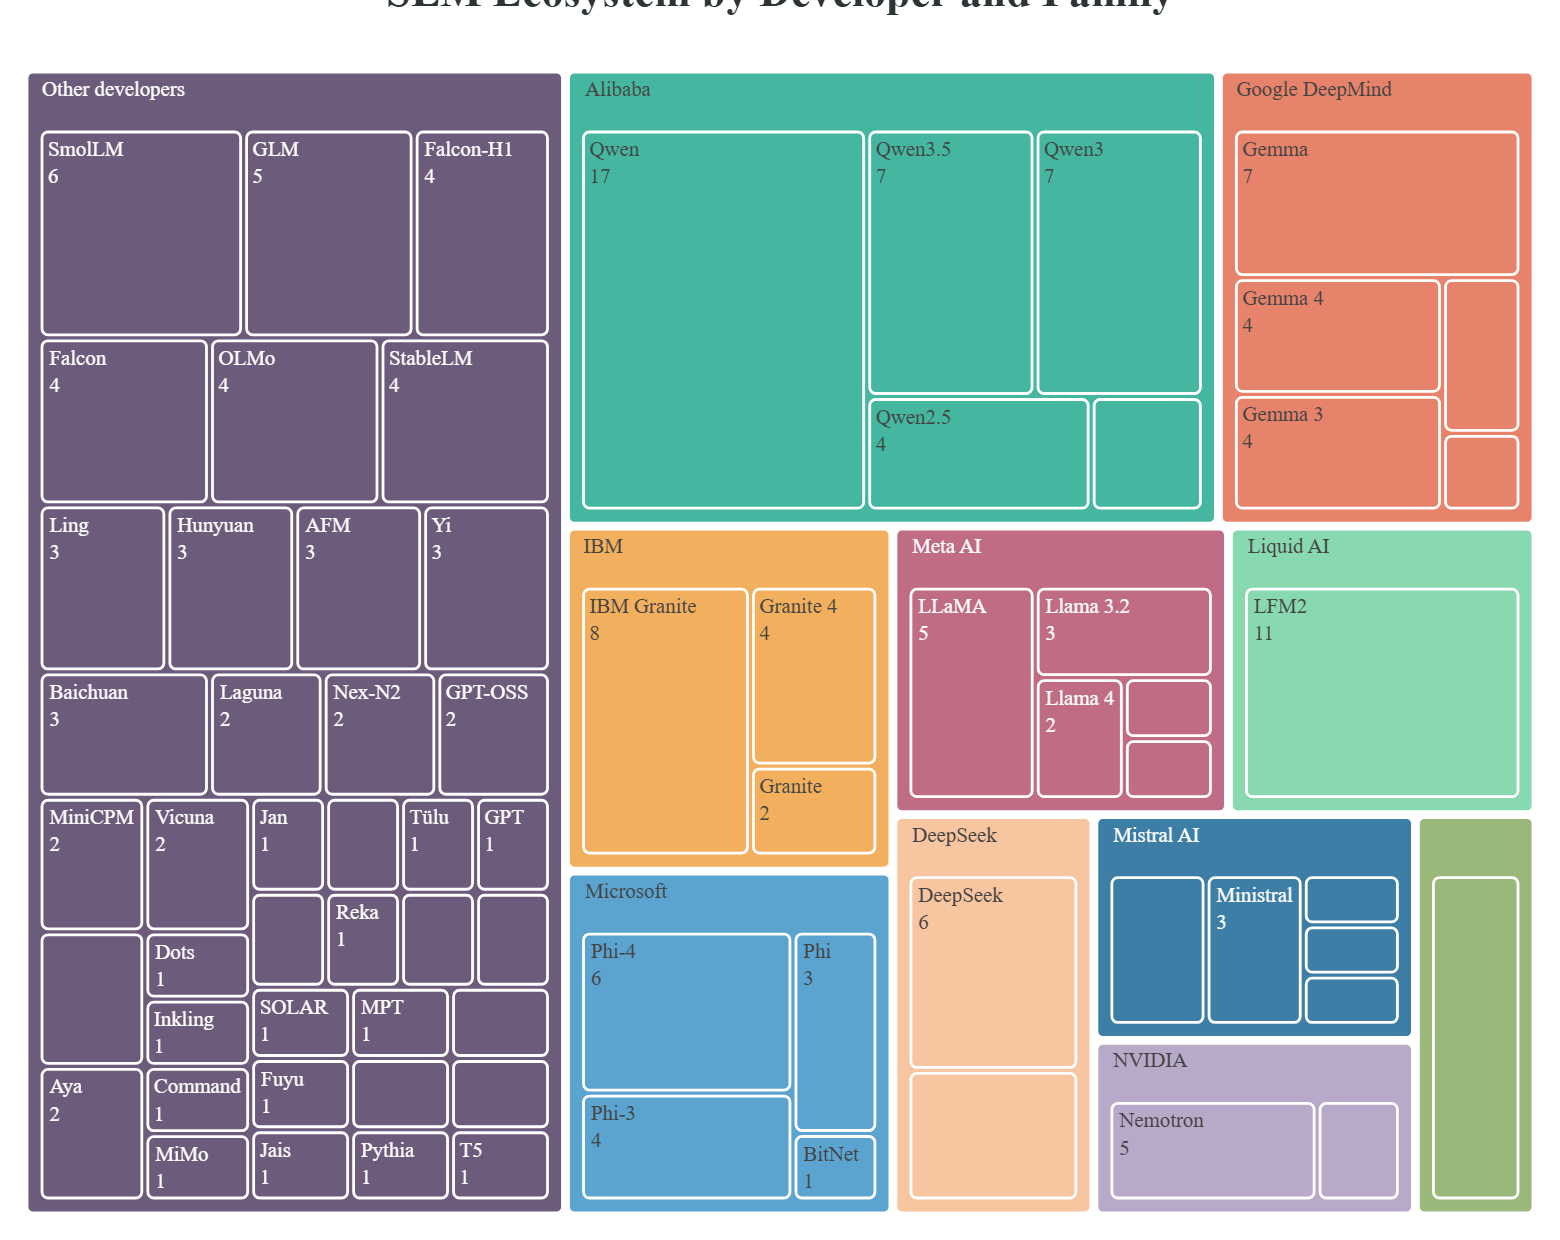
\includegraphics[width=\linewidth]{paper_slm_family_treemap.png}
  \caption{Documented SLM variants grouped by developer and family; area is proportional to the number of variants. Generated from \file{merged\_llm\_database.json} (version~3.6; releases through 4~September 2026).}
  \Description{Treemap of documented small language model variants grouped by developer and then by family, with rectangle area proportional to the number of variants in each group.}
  \label{fig:family_treemap}
\end{figure}

\begin{figure}[ht]
  \centering
  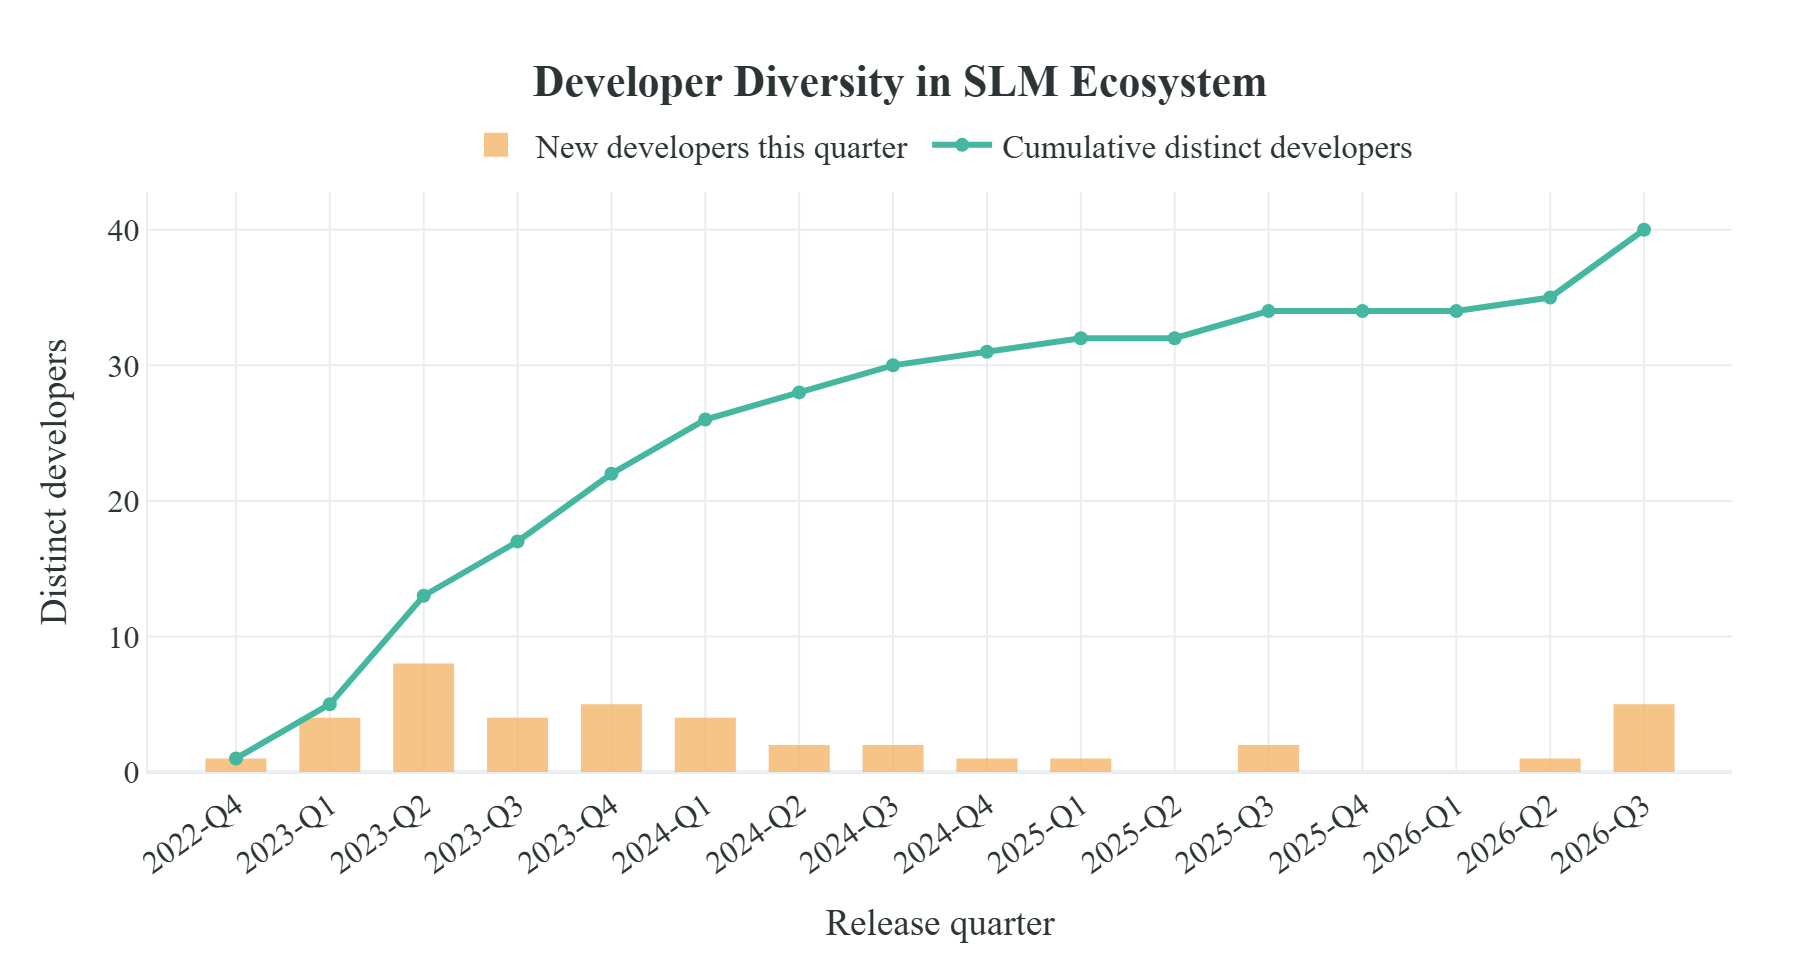
\includegraphics[width=\linewidth]{paper_slm_developer_diversity_timeline.png}
  \caption{Cumulative distinct developers releasing documented SLM variants (line) and new developers per quarter (bars).}
  \Description{Combination chart with bars showing the number of new developers releasing their first documented small language model in each quarter, overlaid with a line showing the cumulative count of distinct developers.}
  \label{fig:developer_diversity}
\end{figure}

\begin{figure}[ht]
  \centering
  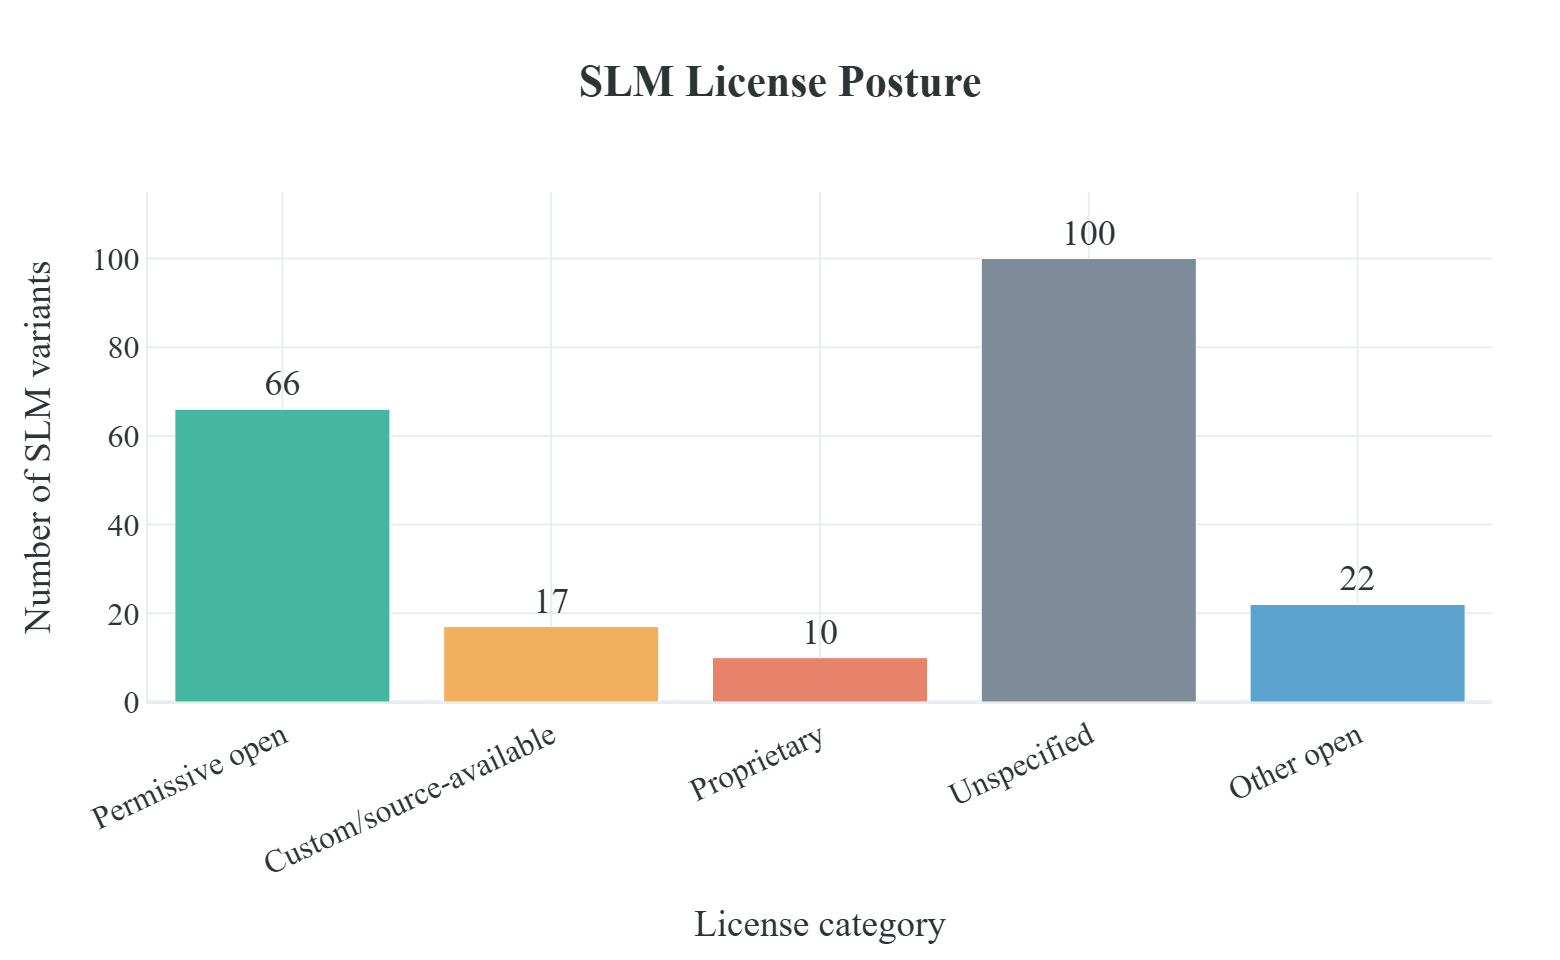
\includegraphics[width=0.78\linewidth]{paper_slm_license_posture.png}
  \caption{License posture of documented SLM variants. Permissive open licenses (Apache-2.0, MIT) account for the plurality; ``unspecified'' entries are typically research checkpoints without an attached license file.}
  \Description{Bar chart of documented small language model variants by license category. Permissive open licenses, chiefly Apache 2.0 and MIT, form the plurality, followed by custom vendor licenses and unspecified research checkpoints.}
  \label{fig:license_posture}
\end{figure}

\subsection{Representative Family Reference}
\label{subsec:ecosystem_families}
Table~\ref{tab:ecosystem_families} lists the representative families tracked in the inventory, with their developers, size ranges, access, and the role each plays in the landscape.

\begin{table}[ht]
\centering
\caption{Representative model families tracked in the inventory.}
\label{tab:ecosystem_families}
\footnotesize\adjustbox{max width=\linewidth}{%
\begin{tabular}{lllll}
\toprule
\textbf{Family} & \textbf{Developer} & \textbf{Representative Versions} & \textbf{Access} & \textbf{Typical Role} \\
\midrule
Qwen2.5 / Qwen3 & Alibaba & 0.5B--14B dense, MoE variants & Open weights & Strong multilingual, math, and code performance \\
Phi-3 / Phi-4 & Microsoft & 3.8B mini variants, 14B reasoning & Open weights & Data-curated reasoning-focused SLMs \\
Gemma 2 / 3 / 3n & Google DeepMind & 1B--12B dense, mobile-first multimodal variants & Open weights & Distilled compact models \\
Llama 3.2 / 4 & Meta & 1B--3B edge models, larger MoE frontier models & Open weights & Broad deployment ecosystem from edge to server \\
SmolLM2 / SmolLM3 & Hugging Face & 135M--3B & Open weights & Lightweight, fully open research and edge baselines \\
DeepSeek distills & DeepSeek & 1.5B--14B distilled reasoning models & Open weights & Reasoning transfer into self-hosted sizes \\
Granite 3 / 4 & IBM & 2--8B dense; 4.0 hybrid Mamba-2/MoE (350M--32B, 1--9B active) & Open weights & Enterprise-friendly, tool-use and RAG focus \\
Falcon-H1 & TII & 0.5--34B parallel attention/Mamba-2 hybrid & Open weights & Long-context edge-to-server \\
LFM2 / LFM2.5 & Liquid AI & 230M--8.3B hybrid conv/attention, incl.\ 8B-A1B MoE & Open weights & CPU-oriented on-device models \\
MiniCPM & OpenBMB & Compact multimodal variants & Open weights & Edge multimodal use cases \\
Ling / Nemotron 3.5 / Laguna & inclusionAI / NVIDIA / Poolside & Small-active MoE, 3--13B active & Open weights & SLM-like per-token cost at LLM-like residency \\
Frontier API families & OpenAI / Anthropic / Google / xAI / others & API frontier models (see released inventory) & API only & High-end proprietary baselines and teacher models \\
\bottomrule
\end{tabular}%
}
\end{table}

\subsection{Classification Conventions}
\label{subsec:ecosystem_classification}
The inventory applies conditions C1 and C2 of Section~\ref{subsubsec:intro_def_operative} from the parameter counts each record carries:
\begin{itemize}
    \item A record enters the inventory when its \emph{active} parameter count is at or below roughly 20B (C1); dense models, for which active equals total, therefore enter at or below 20B total. C2 (total at or below 20B) then separates \glspl{slm} from small-active-parameter \glspl{moe}; both are listed, and only the former carry the paper's storage, resident-memory, and on-device claims.
    \item Where a source states no active-parameter count for a model it describes as a mixture of experts, the record is marked undisclosed rather than having active set equal to total. Nested legacy records are read from their active field.
    \item Per-layer-embedding ``effective'' sizes (Gemma~3n, Gemma~4 E2B/E4B) are not sparse activation; C1 is evaluated on the total and the effective size is kept as a note.
    \item M1 is satisfied when a developer source states size and architecture; the source check of \suppsec~\ref{subsec:source_verification} records which source that is. Records of undisclosed size, whatever their marketing, are kept in the comparison part of the file as \texttt{undisclosed}.
    \item Encoder-decoder models, derivative fine-tunes without a technical report, and API aliases are excluded by named editorial decision and kept under \texttt{models.excluded} with their reason.
\end{itemize}
The count history from 126 to the present 209 is given in \suppsec~\ref{subsec:count_history}, and the released changelog names every record added, moved, or removed at each step.

\subsection{Generated Variant Inventory}
\label{subsec:ecosystem_generated_inventory}
The following inventory is generated directly from \file{merged\_llm\_database.json} using \file{scripts/generate\_model\_tables.py}. Version~3.6 of the database covers 209 inventory records (179 \glspl{slm} and 30 small-active-parameter \glspl{moe}), 223 comparison records (104 of disclosed size that fail C1 and 119 of undisclosed size), and 7 excluded candidates, 439 records in total, for releases through 4~September 2026. Only the inventory is reproduced here (Table~\ref{tab:model_inventory_slm_by_year}), organized by release year and family, with total and, where different, active parameters given in the size column; the comparison records are in the released file.

Each record carries the fields \texttt{meets\_c1\_active\_le\_20b}, \texttt{meets\_c2\_total\_le\_20b}, \texttt{slm\_class}, \texttt{inclusion\_decision}, \texttt{developer\_source\_found}, and \texttt{source\_check}, so that a reader can recompute the inventory under a different threshold, restrict it to models satisfying both conditions, or audit each record's source.

{\footnotesize\noindent\textbf{Chronology.} \hyperref[tab:model_inventory_slm_by_year]{Inventory}: \hyperlink{model-year-slm-2026}{2026}, \hyperlink{model-year-slm-2025}{2025}, \hyperlink{model-year-slm-2024}{2024}, \hyperlink{model-year-slm-2023-and-earlier}{2023 and earlier}.\par}
% Auto-generated by scripts/generate_model_tables.py. Do not edit manually.
\begin{landscape}
{\scriptsize
\setlength{\tabcolsep}{4pt}
\renewcommand{\arraystretch}{1.15}
\begin{longtable}{@{}L{3.3cm}C{1.05cm}L{1.75cm}C{1.15cm}L{2.25cm}L{2.4cm}C{1.6cm}L{3.9cm}@{}}
\caption{Generated chronological small language model inventory from \texttt{merged\_llm\_database.json}, grouped by release year and family. Entries whose parameter column reads ``$N$B ($M$B act.)'' with $N > 20$ are small-active-parameter MoEs (C1 only), not SLMs, and are excluded from every storage and on-device claim.}\label{tab:model_inventory_slm_by_year}\\
\toprule
\textbf{Model} & \textbf{Access} & \textbf{Params} & \textbf{Context} & \textbf{Modalities} & \textbf{License} & \textbf{Release} & \textbf{Notes} \\ \midrule
\endfirsthead
\caption[]{Generated chronological small language model inventory continued.}\\
\toprule
\textbf{Model} & \textbf{Access} & \textbf{Params} & \textbf{Context} & \textbf{Modalities} & \textbf{License} & \textbf{Release} & \textbf{Notes} \\ \midrule
\endhead
\midrule \multicolumn{8}{r@{}}{\footnotesize\itshape continued on next page} \\
\endfoot
\bottomrule
\endlastfoot
\multicolumn{8}{@{}l}{\hypertarget{model-year-slm-2026}{\textbf{2026}}} \\ \midrule
\multicolumn{8}{@{}l}{\textit{Qwen3.5} --- Alibaba (Qwen3.5 (Mar 2026)) \href{https://qwen.ai/blog?id=qwen3.5}{[family page]}} \\*
\href{https://huggingface.co/Qwen/Qwen3.5-0.8B}{Qwen3.5-0.8B} & OW & 0.8B & 256K & Text+Vision+Video & Apache 2.0 & 2026-03-02 & ultra-lightweight multimodal; on-device \\
\href{https://huggingface.co/Qwen/Qwen3.5-2B}{Qwen3.5-2B} & OW & 2B & 256K & Text+Vision+Video & Apache 2.0 & 2026-03-02 & on-device multimodal chat; edge AI \\
\href{https://huggingface.co/Qwen/Qwen3.5-4B}{Qwen3.5-4B} & OW & 4B & 256K & Text+Vision+Video & Apache 2.0 & 2026-03-02 & mobile multimodal assistant; agentic coding \\
\href{https://huggingface.co/Qwen/Qwen3.5-9B}{Qwen3.5-9B} & OW & 9B & 256K & Text+Vision+Video & Apache 2.0 & 2026-03-02 & strong multimodal SLM; coding \\
\href{https://huggingface.co/Qwen/Qwen3.5-35B-A3B}{Qwen3.5-35B-A3B} & OW & 35B (3B act.) & 256K & Text+Vision & Apache 2.0 & 2026-02-16 & efficient MoE for edge/server; multimodal reasoning \\
\href{https://huggingface.co/Qwen/Qwen3.5-122B-A10B}{Qwen3.5-122B-A10B} & OW & 122B (10B act.) & 256K & Text+Vision & Apache 2.0 & 2026-02-16 & strong MoE reasoning; locally runnable flagship \\
\href{https://huggingface.co/Qwen/Qwen3.5-397B-A17B}{Qwen3.5-397B-A17B} & Both & 397B (17B act.) & 256K & Text+Vision & Apache 2.0 & 2026-02-16 & flagship open-weight multimodal; 201 languages \\
\multicolumn{8}{@{}l}{\textit{AFM} --- Apple (AFM) \href{https://machinelearning.apple.com/research/introducing-apple-foundation-models}{[family page]}} \\*
\href{https://machinelearning.apple.com/research/introducing-third-generation-of-apple-foundation-models}{Apple AFM 3 Core Advanced} & API & 20B (1-4B act.) & 64K & Text+Vision & Proprietary & 2026-06-08 & on-device assistant; multimodal understanding \\
\multicolumn{8}{@{}l}{\textit{Command} --- Cohere (Command) \href{https://cohere.com/blog/command-r7b}{[family page]}} \\*
\href{https://huggingface.co/CohereLabs/North-Mini-Code-1.0}{North Mini Code 1.0} & OW & 30B (3B act.) & 250K & Text & CC-BY-NC (Cohere Labs) & 2026-06-17 & coding; agentic coding \\
\multicolumn{8}{@{}l}{\textit{DeepSeek} --- DeepSeek (DeepSeek) \href{https://huggingface.co/deepseek-ai}{[family page]}} \\*
\href{https://huggingface.co/deepseek-ai/DeepSeek-V4-Flash-Vision-Exp}{DeepSeek V4 Flash Vision Exp} & OW & 284B (13B act.) & 1M & Text+Vision & See source & 2026-08-21 & vision; long context \\
\href{https://huggingface.co/deepseek-ai/DeepSeek-V4-Flash-0731}{DeepSeek V4 Flash 0731} & OW & 284B (13B act.) & 1280K & Text & See source & 2026-07-31 & general; long context \\
\multicolumn{8}{@{}l}{\textit{Dots} --- Dots Studio (Dots3-Note Preview (Aug 2026)) \href{https://openrouter.ai/dots-studio/dots-3-note-preview}{[family page]}} \\*
\href{https://huggingface.co/dots-studio/dots3-note-prev}{Dots3-Note Preview} & OW & 280B (16B act.) & 500K & Text & Apache 2.0 & 2026-08-14 & note taking; general \\
\multicolumn{8}{@{}l}{\textit{Gemma 4} --- Google DeepMind} \\*
\href{https://huggingface.co/google/gemma-4-26B}{Gemma 4 26B (MoE)} & OW & 26B (3.8B act.) & 128K & Text+Vision & Apache 2.0 & 2026-04-02 & reasoning; multimodal \\
\href{https://huggingface.co/google/gemma-4-E2B}{Gemma 4 E2B} & OW & \textasciitilde{}5B & 128K & Text+Vision+Audio & Apache 2.0 & 2026-04-02 & on-device; multimodal \\
\href{https://huggingface.co/google/gemma-4-E4B}{Gemma 4 E4B} & OW & \textasciitilde{}8B & 128K & Text+Vision+Audio & Apache 2.0 & 2026-04-02 & multimodal; reasoning \\
\href{https://huggingface.co/google/gemma-4-12b}{Gemma 4 12B} & OW & 12B & 256K & Text+Vision+Audio & Apache 2.0 & 2026-04-02 & multimodal; reasoning \\
\multicolumn{8}{@{}l}{\textit{Granite 4} --- IBM} \\*
\href{https://huggingface.co/ibm-granite/granite-4.2-3b}{Granite 4.2 3B} & OW & 3B & 128K & Text & Apache 2.0 & 2026-08-25 & reasoning; on-device \\
\href{https://huggingface.co/ibm-granite/granite-4.2-8b}{Granite 4.2 8B} & OW & 8B & 128K & Text & Apache 2.0 & 2026-08-25 & reasoning; agentic \\
\href{https://huggingface.co/ibm-granite/granite-4.1-3b}{Granite 4.1 3B} & OW & 3B & 128K & Text & Apache 2.0 & 2026-04-29 & enterprise; on-device \\
\href{https://huggingface.co/ibm-granite/granite-4.1-8b}{Granite 4.1 8B} & OW & 8B & 128K & Text & Apache 2.0 & 2026-04-29 & enterprise; agentic \\
\multicolumn{8}{@{}l}{\textit{LFM2} --- Liquid AI} \\*
\href{https://huggingface.co/LiquidAI/LFM2.5-2.6B}{LFM2.5-2.6B} & Both & 2.69B & 128K & Text & LFM1.0 & 2026-08-04 & agentic workflows; data extraction \\
\href{https://www.liquid.ai/blog/lfm2-5-8b-a1b}{LFM2.5-8B-A1B} & OW & 8.3B (1.5B act.) & 128K & Text & LFM1.0 & 2026-05-28 & on-device; tool calling \\
\href{https://www.liquid.ai/blog/lfm2-5-350m-no-size-left-behind}{LFM2.5-350M} & OW & 350M & 128K & Text & LFM1.0 & 2026 & on-device; edge \\
\href{https://www.liquid.ai/models}{LFM2.5-1.2B} & OW & 1.2B & 128K & Text & LFM1.0 & 2026 & on-device; edge \\
\href{https://www.liquid.ai/models}{LFM2.5-Audio-1.5B} & OW & 1.5B & -- & Text+Audio & LFM1.0 & 2026 & on-device speech; transcription \\
\href{https://www.liquid.ai/models}{LFM2.5-VL-3B} & OW & 3B & -- & Text+Vision & LFM1.0 & 2026 & on-device VLM; document extraction \\
\multicolumn{8}{@{}l}{\textit{Mistral Small} --- Mistral AI (Mistral Small 4 (Mar 2026)) \href{https://mistral.ai/news/mistral-small-4}{[family page]}} \\*
\href{https://huggingface.co/mistralai/Mistral-Small-4-119B-2603}{Mistral Small 4 (119B)} & Both & 119B (6.5B act.) & 256K & Text+Vision & Apache 2.0 & 2026-03-16 & hybrid reasoning; coding \\
\multicolumn{8}{@{}l}{\textit{NVIDIA Nemotron} --- NVIDIA (Nemotron 3 Super (Mar 2026)) \href{https://developer.nvidia.com/blog/introducing-nemotron-3-super-an-open-hybrid-mamba-transformer-moe-for-agentic-reasoning/}{[family page]}} \\*
\href{https://huggingface.co/nvidia/NVIDIA-NemotronLabs-VoiceChat-11B}{NemotronLabs VoiceChat 11B} & OW & 11B & 128K & Text+Audio & NVIDIA Custom & 2026-08-03 & voice interaction; on-device speech \\
\href{https://huggingface.co/nvidia/NVIDIA-Nemotron-3-Super-120B-A12B-BF16}{Nemotron 3 Super} & OW & 120B (12B act.) & 1M & Text & NVIDIA Open Model License & 2026-03 & open hybrid Mamba-Transformer MoE; agentic reasoning \\
\multicolumn{8}{@{}l}{\textit{Nemotron} --- NVIDIA (Nemotron) \href{https://arxiv.org/abs/2402.16819}{[family page]}} \\*
\href{https://huggingface.co/nvidia/NVIDIA-Nemotron-3.5-Lightning-30B-A3B-BF16}{Nemotron 3.5 Lightning 30B-A3B} & OW & 30B (3B act.) & 256K & Text & NVIDIA Open Model License & 2026-08-11 & agentic execution layer; high-volume tool calling \\
\href{https://huggingface.co/nvidia/Nemotron-3.5-Content-Safety}{Nemotron 3.5 Content Safety} & OW & 4B & 128K & Text+Vision & NVIDIA Open Model License & 2026-06-04 & guardrails; content moderation \\
\multicolumn{8}{@{}l}{\textit{Nex-N2} --- Nex AGI (Nex-N2-Mini (Jun 2026)) \href{https://huggingface.co/nex-agi/Nex-N2-Pro}{[family page]}} \\*
\href{https://huggingface.co/nex-agi/Nex-N2-Pro}{Nex-N2-Pro} & OW & 397B (17B act.) & 256K & Text+Vision & See source & 2026-06-08 & agentic; coding \\
\multicolumn{8}{@{}l}{\textit{Laguna} --- Poolside (Laguna S 2.1 (Jul 2026)) \href{https://poolside.ai/}{[family page]}} \\*
\href{https://huggingface.co/poolside/Laguna-S-2.1}{Laguna S 2.1} & OW & 118B (8B act.) & 1M & Text & See source & 2026-07-21 & coding agent \\
\href{https://huggingface.co/poolside/Laguna-XS-2.1}{Laguna XS 2.1} & OW & 33B (3B act.) & 256K & Text & See source & 2026-07-02 & coding agent \\
\multicolumn{8}{@{}l}{\textit{Hunyuan} --- Tencent (Hunyuan) \href{https://huggingface.co/tencent/Tencent-Hunyuan-Large}{[family page]}} \\*
\href{https://huggingface.co/tencent/Hy-MT2-1.8B}{Hy-MT2-1.8B} & OW & 1.8B & 8K & Text & Tencent Hunyuan License & 2026-08-20 & translation; on-device \\
\href{https://huggingface.co/tencent/Hy-MT2-30B-A3B}{Hy-MT2-30B-A3B} & OW & 30B (3B act.) & 8K & Text & Tencent Hunyuan License & 2026-08-20 & translation \\
\href{https://huggingface.co/tencent/Hy-MT2-7B}{Hy-MT2-7B} & OW & 7B & 8K & Text & Tencent Hunyuan License & 2026-08-19 & translation; Lang: 33 language pairs + 5 dialect/minority pairs \\
\multicolumn{8}{@{}l}{\textit{Inkling} --- Thinking Machines Lab (Inkling Small (Jul 2026)) \href{https://huggingface.co/thinkingmachines/Inkling}{[family page]}} \\*
\href{https://huggingface.co/thinkingmachines/Inkling-Small}{Inkling Small} & OW & 276B (12B act.) & 1M & Text+Vision & See source & 2026-07-30 & general; multimodal \\
\multicolumn{8}{@{}l}{\textit{MiMo} --- Xiaomi (MiMo-V2-Pro (Mar 2026)) \href{https://mimo.xiaomi.com/mimo-v2-pro}{[family page]}} \\*
\href{https://huggingface.co/XiaomiMiMo/MiMo-V2-Flash}{MiMo-V2-Flash} & OW & 309B (15B act.) & 256K & Text & Undisclosed & 2026 & high-throughput coding agents; production serving \\
\multicolumn{8}{@{}l}{\textit{Ling} --- inclusionAI (Ling-1T (2026)) \href{https://huggingface.co/01ai/Ling-1T}{[family page]}} \\*
\href{https://huggingface.co/inclusionAI/Ling-3.0-flash-Fin}{Ling 3.0 Flash Fin} & OW & 124B (5.1B act.) & 256K & Text & MIT & 2026-08-27 & finance \\
\href{https://huggingface.co/inclusionAI/Ling-3.0-flash}{Ling 3.0 Flash} & OW & 124B (5.1B act.) & 256K & Text & See source & 2026-07-23 & general; agentic \\
\addlinespace[3pt]
\multicolumn{8}{@{}l}{\hypertarget{model-year-slm-2025}{\textbf{2025}}} \\ \midrule
\multicolumn{8}{@{}l}{\textit{Qwen} --- Alibaba (Qwen) \href{https://github.com/QwenLM/Qwen}{[family page]}} \\*
\href{https://huggingface.co/Qwen/Qwen2.5-Omni-7B}{Qwen2.5-Omni-7B} & OW & 7B & -- & Text+Audio+Video+Image & See source & 2025-03-26 & omni-modal; text and audio output \\
\href{https://huggingface.co/Qwen/Qwen2.5-VL-7B-Instruct}{Qwen2.5-VL-7B} & OW & 7B & -- & Text+Video+Image & See source & 2025-01-22 & active \\
\multicolumn{8}{@{}l}{\textit{Qwen3} --- Alibaba (Qwen3 (Apr 2025)) \href{https://github.com/QwenLM/Qwen3}{[family page]}} \\*
\href{https://huggingface.co/Qwen/Qwen3-4B-Instruct-2507}{Qwen3-4B-Instruct-2507} & OW & 4B & 128K & Text & Apache 2.0 & 2025-07 & improved instruction following; non-thinking mode optimised \\
\href{https://huggingface.co/Qwen/Qwen3-0.6B}{Qwen3-0.6B} & OW & 0.6B & 32K & Text & Apache 2.0 & 2025-04-29 & edge inference; IoT \\
\href{https://huggingface.co/Qwen/Qwen3-1.7B}{Qwen3-1.7B} & OW & 1.7B & 32K & Text & Apache 2.0 & 2025-04-29 & mobile inference; Q\&A \\
\href{https://huggingface.co/Qwen/Qwen3-30B-A3B}{Qwen3-30B-A3B} & OW & 30B (3B act.) & 128K & Text & Apache 2.0 & 2025-04-29 & MoE efficiency; broad capability in tiny footprint \\
\href{https://huggingface.co/Qwen/Qwen3-4B-Instruct}{Qwen3-4B-Instruct} & OW & 4B & 128K & Text & Apache 2.0 & 2025-04-29 & on-device chat; coding \\
\href{https://huggingface.co/Qwen/Qwen3-8B-Instruct}{Qwen3-8B-Instruct} & OW & 8B & 128K & Text & Apache 2.0 & 2025-04-29 & single-GPU inference; reasoning \\
\href{https://huggingface.co/Qwen/Qwen3-14B-Instruct}{Qwen3-14B-Instruct} & OW & 14B & 128K & Text & Apache 2.0 & 2025-04-29 & high-quality on-premise chat; coding \\
\multicolumn{8}{@{}l}{\textit{AFM} --- Apple (AFM) \href{https://machinelearning.apple.com/research/introducing-apple-foundation-models}{[family page]}} \\*
\href{https://arxiv.org/abs/2507.13575}{Apple Foundation Model (On-Device, 2nd gen)} & API & \textasciitilde{}3B & 64K & Text+Vision & Proprietary & 2025-06-09 & on-device assistant; writing tools \\
\multicolumn{8}{@{}l}{\textit{DeepSeek R1-Distill} --- DeepSeek (R1-Distill (Jan 2025)) \href{https://huggingface.co/deepseek-ai}{[family page]}} \\*
\href{https://huggingface.co/deepseek-ai/DeepSeek-R1-Distill-Qwen-1.5B}{DeepSeek-R1-Distill-Qwen-1.5B} & OW & 1.5B & 128K & Text & MIT & 2025-01-20 & reasoning at ultra-small scale; math \\
\href{https://huggingface.co/deepseek-ai/DeepSeek-R1-Distill-Qwen-7B}{DeepSeek-R1-Distill-Qwen-7B} & OW & 7B & 128K & Text & MIT & 2025-01-20 & chain-of-thought reasoning; coding \\
\href{https://huggingface.co/deepseek-ai/DeepSeek-R1-Distill-Llama-8B}{DeepSeek-R1-Distill-Llama-8B} & OW & 8B & 128K & Text & MIT & 2025-01-20 & reasoning on Llama 3 base; on-premise \\
\href{https://huggingface.co/deepseek-ai/DeepSeek-R1-Distill-Qwen-14B}{DeepSeek-R1-Distill-Qwen-14B} & OW & 14B & 128K & Text & MIT & 2025-01-20 & strong reasoning 14B; top distill for coding \\
\multicolumn{8}{@{}l}{\textit{Gemma 3} --- Google DeepMind (Gemma 3 (Mar 2025)) \href{https://huggingface.co/blog/gemma3}{[family page]}} \\*
\href{https://huggingface.co/google/gemma-3-270m-it}{Gemma 3 270M-IT} & OW & 270M & 32K & Text & Google Gemma License & 2025-03 & ultra-lightweight prototyping; experiments \\
\href{https://huggingface.co/google/gemma-3-1b-it}{Gemma 3 1B-IT} & OW & 1B & 32K & Text & Google Gemma License & 2025-03 & on-device mobile inference; lightweight Q\&A \\
\href{https://huggingface.co/google/gemma-3-4b-it}{Gemma 3 4B-IT} & OW & 4B & 128K & Text+Vision & Google Gemma License & 2025-03 & multimodal on-device; image understanding \\
\href{https://huggingface.co/google/gemma-3-12b-it}{Gemma 3 12B-IT} & OW & 12B & 128K & Text+Vision & Google Gemma License & 2025-03 & high-quality assistant; 140+ languages \\
\multicolumn{8}{@{}l}{\textit{Gemma 3n} --- Google DeepMind (Gemma-3n (2025)) \href{https://ai.google.dev/gemma/docs/gemma-3n}{[family page]}} \\*
\href{https://huggingface.co/google/gemma-3n-E2B-it}{Gemma-3n-E2B-IT} & OW & \textasciitilde{}5B & 32K & Text+Vision+Audio+Video & Google Gemma License & 2025 & mobile-first multimodal; on-device speech/vision/text \\
\href{https://huggingface.co/google/gemma-3n-E4B-it}{Gemma-3n-E4B-IT} & OW & \textasciitilde{}8B & 32K & Text+Vision+Audio+Video & Google Gemma License & 2025 & higher-accuracy mobile multimodal; edge devices \\
\multicolumn{8}{@{}l}{\textit{SmolLM} --- Hugging Face (SmolLM3-3B (2025)) \href{https://huggingface.co/HuggingFaceTB/SmolLM3-3B}{[family page]}} \\*
\href{https://huggingface.co/HuggingFaceTB/SmolLM3-3B}{SmolLM3-3B} & OW & 3B & 64K & Text & Apache 2.0 & 2025 & dual-mode reasoning; tool calling \\
\multicolumn{8}{@{}l}{\textit{Granite} --- IBM (Granite) \href{https://huggingface.co/ibm-granite}{[family page]}} \\*
\href{https://huggingface.co/ibm-granite/granite-3.2-2b-instruct}{Granite 3.2-2B} & OW & 2B & 125K & Text & See source & 2025-02-26 & Thinking mode; 128K context \\
\href{https://huggingface.co/ibm-granite/granite-3.2-8b-instruct}{Granite 3.2-8B} & OW & 8B & 125K & Text & See source & 2025-02-26 & Thinking mode (chain-of-thought); 128K context \\
\multicolumn{8}{@{}l}{\textit{IBM Granite} --- IBM (Granite 3.3 (Apr 2025)) \href{https://huggingface.co/ibm-granite}{[family page]}} \\*
\href{https://huggingface.co/ibm-granite/granite-4.0-nano-350m}{Granite 4.0 Nano 350M} & OW & 350M & 128K & Text & Apache 2.0 & 2025-10-28 & on-device; browser \\
\href{https://huggingface.co/ibm-granite/granite-4.0-nano-1b}{Granite 4.0 Nano 1B} & OW & 1B & 128K & Text & Apache 2.0 & 2025-10-28 & on-device; browser \\
\href{https://huggingface.co/ibm-granite/granite-4.0-h-tiny}{Granite 4.0 H-Tiny} & OW & 7B (1B act.) & 128K & Text & Apache 2.0 & 2025-10-02 & low-latency; agentic \\
\href{https://huggingface.co/ibm-granite/granite-4.0-h-micro}{Granite 4.0 H-Micro} & OW & 3B & 128K & Text & Apache 2.0 & 2025-10-02 & edge; tool use \\
\href{https://huggingface.co/ibm-granite/granite-4.0-micro}{Granite 4.0 Micro} & OW & 3B & 128K & Text & Apache 2.0 & 2025-10-02 & edge; RAG \\
\href{https://huggingface.co/ibm-granite/granite-4.0-h-small}{Granite 4.0 H-Small} & OW & 32B (9B act.) & 128K & Text & Apache 2.0 & 2025-10-02 & enterprise; agentic \\
\href{https://huggingface.co/ibm-granite/granite-3.3-2b-instruct}{Granite 3.3-2B-Instruct} & OW & 2B & 128K & Text & Apache 2.0 & 2025-04 & enterprise NLP; governed AI \\
\href{https://huggingface.co/ibm-granite/granite-3.3-8b-instruct}{Granite 3.3-8B-Instruct} & OW & 8B & 128K & Text & Apache 2.0 & 2025-04 & enterprise reasoning; Fill-in-Middle code \\
\multicolumn{8}{@{}l}{\textit{LFM2} --- Liquid AI} \\*
\href{https://huggingface.co/LiquidAI/LFM2-8B-A1.5B}{LFM2-8B-A1.5B (MoE)} & OW & 8.3B (1.5B act.) & 32K & Text & LFM Open License v1.0 & 2025-08 & on-device; agentic \\
\href{https://huggingface.co/LiquidAI/LFM2-2.6B}{LFM2-2.6B} & OW & 2.6B & 32K & Text & LFM Open License v1.0 & 2025-08 & on-device \\
\href{https://huggingface.co/LiquidAI/LFM2-350M}{LFM2-350M} & OW & 350M & 32K & Text & LFM Open License v1.0 & 2025-07-10 & on-device; low latency \\
\href{https://huggingface.co/LiquidAI/LFM2-700M}{LFM2-700M} & OW & 700M & 32K & Text & LFM Open License v1.0 & 2025-07-10 & on-device \\
\href{https://huggingface.co/LiquidAI/LFM2-1.2B}{LFM2-1.2B} & OW & 1.2B & 32K & Text & LFM Open License v1.0 & 2025-07-10 & on-device; agentic \\
\multicolumn{8}{@{}l}{\textit{Llama 4} --- Meta AI (Llama 4 Maverick (Apr 2025)) \href{https://ai.meta.com/blog/llama-4-multimodal-intelligence/}{[family page]}} \\*
\href{https://huggingface.co/meta-llama/Llama-4-Maverick-17B-128E-Instruct}{Llama 4 Maverick} & Both & 400B (17B act.) & 10M & Text+Vision & Llama 4 Community License & 2025-04-05 & image understanding; coding \\
\href{https://huggingface.co/meta-llama/Llama-4-Scout-17B-16E-Instruct}{Llama 4 Scout} & Both & 109B (17B act.) & 10M & Text+Vision & Llama 4 Community License & 2025-04-05 & extreme long-context; single H100 runnable \\
\multicolumn{8}{@{}l}{\textit{BitNet} --- Microsoft (BitNet) \href{https://arxiv.org/abs/2402.17764}{[family page]}} \\*
\href{https://huggingface.co/microsoft/bitnet-b1.58-2B-4T}{BitNet b1.58 2B4T} & OW & 2B & -- & Text & MIT & 2025-04-16 & 1-bit LLM (ternary weights: -1, 0, 1); Extreme efficiency \\
\multicolumn{8}{@{}l}{\textit{Phi-4} --- Microsoft (Phi-4-reasoning-plus (Apr 2025)) \href{https://huggingface.co/microsoft/phi-4}{[family page]}} \\*
\href{https://huggingface.co/microsoft/Phi-4-mini-flash-reasoning}{Phi-4-mini-flash-reasoning} & OW & 3.8B & 128K & Text & MIT & 2025-04 & fast reasoning; edge agents \\
\href{https://huggingface.co/microsoft/Phi-4-mini-reasoning}{Phi-4-mini-reasoning} & OW & 3.8B & 128K & Text & MIT & 2025-04 & chain-of-thought reasoning; math \\
\href{https://huggingface.co/microsoft/Phi-4-reasoning}{Phi-4-reasoning} & OW & 14B & 128K & Text & MIT & 2025-04 & complex reasoning; STEM \\
\href{https://huggingface.co/microsoft/Phi-4-reasoning-plus}{Phi-4-reasoning-plus} & OW & 14B & 128K & Text & MIT & 2025-04 & RL-trained reasoning; math olympiad-level \\
\href{https://huggingface.co/microsoft/Phi-4-mini-instruct}{Phi-4-mini-instruct} & OW & 3.8B & 128K & Text & MIT & 2025-02 & on-device chat; function calling \\
\multicolumn{8}{@{}l}{\textit{Ministral} --- Mistral AI (Ministral-3B (Dec 2025)) \href{https://docs.mistral.ai/getting-started/models}{[family page]}} \\*
\href{https://huggingface.co/mistralai/Ministral-3-14B-Instruct-2512}{Ministral 3 (14B)} & OW & 14B & -- & Text+Vision & See source & 2025-12-02 & edge deployment; multimodal \\
\href{https://huggingface.co/mistralai/Ministral-3B-instruct-2512}{Ministral-3B-Instruct-2512} & OW & 3.8B & 256K & Text+Vision & Apache 2.0 & 2025-12 & tiny multimodal; function calling \\
\multicolumn{8}{@{}l}{\textit{Voxtral} --- Mistral AI (Voxtral) \href{https://mistral.ai/models}{[family page]}} \\*
\href{https://huggingface.co/mistralai/Voxtral-Mini-3B-2507}{Voxtral Mini 3B} & OW & 4.7B & -- & Text+Audio & Apache 2.0 & 2025-07-15 & speech understanding; transcription \\
\multicolumn{8}{@{}l}{\textit{Nemotron} --- NVIDIA (Nemotron) \href{https://arxiv.org/abs/2402.16819}{[family page]}} \\*
\href{https://huggingface.co/nvidia/Nemotron-3-Nano-30B}{Nemotron 3 Nano-30B} & OW & 30B & -- & Text & See source & 2025-12-15 & hybrid Mamba-Transformer MoE; 1M context \\
\href{https://huggingface.co/nvidia/NVIDIA-Nemotron-Nano-9B-v2}{NVIDIA Nemotron Nano 2} & OW & 9B & 128K & Text & See source & 2025-08-18 & on-device; efficient \\
\multicolumn{8}{@{}l}{\textit{GPT-OSS} --- OpenAI (gpt-oss-120b (2025)) \href{https://openai.com/index/introducing-gpt-oss/}{[family page]}} \\*
\href{https://huggingface.co/openai/gpt-oss-20b}{gpt-oss-20b} & OW & 21B (3.6B act.) & 128K & Text & Apache 2.0 & 2025 & edge reasoning; 16GB device inference \\
\href{https://huggingface.co/openai/gpt-oss-120b}{gpt-oss-120b} & OW & 117B (5.1B act.) & 128K & Text & Apache 2.0 & 2025 & open-weight reasoning; near o4-mini parity \\
\multicolumn{8}{@{}l}{\textit{MiniCPM} --- OpenBMB (MiniCPM-V 4.5 (2025)) \href{https://github.com/OpenBMB/MiniCPM-V}{[family page]}} \\*
\href{https://huggingface.co/openbmb/MiniCPM-V-4\_5}{MiniCPM-V 4.5} & OW & \textasciitilde{}8B & 32K & Text+Vision & Apache 2.0 & 2025 & mobile vision-language; on-device VQA \\
\href{https://github.com/OpenBMB/MiniCPM-o}{MiniCPM-o 3.0} & OW & \textasciitilde{}9B & 32K & Text+Vision+Audio & Apache 2.0 & 2025 & end-to-end multimodal on-device; live streaming \\
\multicolumn{8}{@{}l}{\textit{InternLM} --- Shanghai AI Laboratory (InternLM) \href{https://github.com/InternLM/InternLM}{[family page]}} \\*
\href{https://huggingface.co/internlm/internlm3-8b-instruct}{InternLM3-8B} & OW & 8B & 32K & Text & See source & 2025-01-09 & Reasoning via deep thinking; Knowledge-rich training pipeline \\
\multicolumn{8}{@{}l}{\textit{Falcon-H1} --- Technology Innovation Institute} \\*
\href{https://huggingface.co/tiiuae/Falcon-H1-0.5B-Instruct}{Falcon-H1-0.5B} & OW & 0.5B & 256K & Text & Falcon-LLM License 2.0 & 2025-07-31 & edge; long context \\
\href{https://huggingface.co/tiiuae/Falcon-H1-1.5B-Instruct}{Falcon-H1-1.5B} & OW & 1.5B & 256K & Text & Falcon-LLM License 2.0 & 2025-07-31 & edge; long context \\
\href{https://huggingface.co/tiiuae/Falcon-H1-3B-Instruct}{Falcon-H1-3B} & OW & 3B & 256K & Text & Falcon-LLM License 2.0 & 2025-07-31 & general; long context \\
\href{https://huggingface.co/tiiuae/Falcon-H1-7B-Instruct}{Falcon-H1-7B} & OW & 7B & 256K & Text & Falcon-LLM License 2.0 & 2025-07-31 & general; long context \\
\addlinespace[3pt]
\multicolumn{8}{@{}l}{\hypertarget{model-year-slm-2024}{\textbf{2024}}} \\ \midrule
\multicolumn{8}{@{}l}{\textit{Yi} --- 01.AI (Yi) \href{https://huggingface.co/01-ai/Yi-6B}{[family page]}} \\*
\href{https://huggingface.co/01-ai/Yi-1.5-6B}{Yi-1.5-6B} & OW & 6B & -- & Text & See source & 2024-05-13 & legacy \\
\href{https://huggingface.co/01-ai/Yi-1.5-9B}{Yi-1.5-9B} & OW & 9B & -- & Text & See source & 2024-05-13 & legacy \\
\multicolumn{8}{@{}l}{\textit{Qwen} --- Alibaba (Qwen) \href{https://github.com/QwenLM/Qwen}{[family page]}} \\*
\href{https://huggingface.co/Qwen/Qwen2.5-Coder-1.5B-Instruct}{Qwen2.5-Coder-1.5B} & OW & 1.5B & -- & Text & See source & 2024-11-12 & compact coding model \\
\href{https://huggingface.co/Qwen/Qwen2.5-14B}{Qwen2.5-14B} & OW & 14B & -- & Text & See source & 2024-09-19 & active \\
\href{https://huggingface.co/Qwen/Qwen2-VL-7B-Instruct}{Qwen2-VL-7B} & OW & 7B & -- & Text+Video+Image & See source & 2024-08-28 & vision-language; video understanding \\
\href{https://huggingface.co/Qwen/Qwen2-Audio-7B-Instruct}{Qwen2-Audio-7B} & OW & 7B & -- & Text+Audio & See source & 2024-08-09 & audio understanding; speech recognition \\
\href{https://huggingface.co/Qwen/Qwen2-0.5B}{Qwen2-0.5B} & OW & 0.5B & -- & Text & See source & 2024-06-07 & active \\
\href{https://huggingface.co/Qwen/Qwen2-1.5B}{Qwen2-1.5B} & OW & 1.5B & -- & Text & See source & 2024-06-07 & active \\
\href{https://huggingface.co/Qwen/Qwen2-7B}{Qwen2-7B} & OW & 7B & -- & Text & See source & 2024-06-07 & active \\
\href{https://huggingface.co/Qwen/Qwen2-57B-A14B}{Qwen2-57B-A14B} & OW & 57B & -- & Text & See source & 2024-06-07 & active \\
\href{https://huggingface.co/Qwen/Qwen1.5-MoE-A2.7B}{Qwen1.5-MoE-A2.7B} & OW & 14.3B & -- & Text & See source & 2024-03-28 & MoE architecture; efficient \\
\href{https://huggingface.co/Qwen/Qwen1.5-0.5B}{Qwen1.5-0.5B} & OW & 0.5B & -- & Text & See source & 2024-02-05 & legacy \\
\href{https://huggingface.co/Qwen/Qwen1.5-7B}{Qwen1.5-7B} & OW & 7B & -- & Text & See source & 2024-02-05 & legacy \\
\href{https://huggingface.co/Qwen/Qwen1.5-14B}{Qwen1.5-14B} & OW & 14B & -- & Text & See source & 2024-02-05 & legacy \\
\multicolumn{8}{@{}l}{\textit{Qwen2.5} --- Alibaba (Qwen2.5 (Sep 2024)) \href{https://huggingface.co/Qwen}{[family page]}} \\*
\href{https://huggingface.co/Qwen/Qwen2.5-0.5B-Instruct}{Qwen2.5-0.5B-Instruct} & OW & 0.5B & 32K & Text & Apache 2.0 & 2024-09-19 & extreme edge/IoT; classification \\
\href{https://huggingface.co/Qwen/Qwen2.5-1.5B-Instruct}{Qwen2.5-1.5B-Instruct} & OW & 1.5B & 32K & Text & Apache 2.0 & 2024-09-19 & edge NLP; lightweight assistants \\
\href{https://huggingface.co/Qwen/Qwen2.5-3B-Instruct}{Qwen2.5-3B-Instruct} & OW & 3B & 32K & Text & Apache 2.0 & 2024-09-19 & mobile chat; summarization \\
\href{https://huggingface.co/Qwen/Qwen2.5-7B-Instruct}{Qwen2.5-7B-Instruct} & OW & 7B & 128K & Text & Apache 2.0 & 2024-09-19 & general assistant; coding \\
\multicolumn{8}{@{}l}{\textit{Qwen2.5-Coder} --- Alibaba (Qwen2.5-Coder (Nov 2024)) \href{https://huggingface.co/Qwen/Qwen2.5-Coder-7B-Instruct}{[family page]}} \\*
\href{https://huggingface.co/Qwen/Qwen2.5-Coder-7B-Instruct}{Qwen2.5-Coder-7B-Instruct} & OW & 7B & 128K & Text+Code & Apache 2.0 & 2024-11 & code generation; debugging \\
\href{https://huggingface.co/Qwen/Qwen2.5-Coder-14B-Instruct}{Qwen2.5-Coder-14B-Instruct} & OW & 14B & 128K & Text+Code & Apache 2.0 & 2024-11 & advanced code assistant; agentic code tasks \\
\multicolumn{8}{@{}l}{\textit{OLMo} --- Allen Institute for AI (Ai2) (OLMo) \href{https://allenai.org/olmo}{[family page]}} \\*
\href{https://huggingface.co/allenai/OLMo-2-1124-7B}{OLMo 2-7B} & OW & 7B & -- & Text & See source & 2024-11-26 & fully open; training code included \\
\href{https://huggingface.co/allenai/OLMo-2-1124-13B}{OLMo 2-13B} & OW & 13B & -- & Text & See source & 2024-11-26 & active \\
\href{https://huggingface.co/allenai/OLMo-1B}{OLMo-1B} & OW & 1B & 2K & Text & See source & 2024-02-01 & Fully open (data, code, weights, logs); Dolma training data \\
\href{https://huggingface.co/allenai/OLMo-7B}{OLMo-7B} & OW & 7B & -- & Text & See source & 2024-02-01 & fully open; training data/code/logs released \\
\multicolumn{8}{@{}l}{\textit{Tülu} --- Allen Institute for AI (Ai2) (Tülu) \href{https://allenai.org/blog/tulu-3-technical}{[family page]}} \\*
\href{https://huggingface.co/allenai/Llama-3.1-Tulu-3-8B}{Tülu 3-8B} & OW & 8B & -- & Text & See source & 2024-11-22 & instruction following; DPO \\
\multicolumn{8}{@{}l}{\textit{AFM} --- Apple (AFM) \href{https://machinelearning.apple.com/research/introducing-apple-foundation-models}{[family page]}} \\*
\href{https://machinelearning.apple.com/research/introducing-apple-foundation-models}{Apple Foundation Model (On-Device)} & API & \textasciitilde{}3B & 4K & Text & Proprietary & 2024-06-10 & On-device Apple Intelligence; Privacy-preserving \\
\multicolumn{8}{@{}l}{\textit{OpenELM} --- Apple (OpenELM) \href{https://machinelearning.apple.com/research/openelm}{[family page]}} \\*
\href{https://huggingface.co/apple/OpenELM-3B}{OpenELM} & OW & 3B & -- & Text & See source & 2024-04-24 & layer-wise scaling; on-device \\
\multicolumn{8}{@{}l}{\textit{Aya} --- Cohere (Aya) \href{https://cohere.com/research/aya}{[family page]}} \\*
\href{https://huggingface.co/CohereForAI/aya-expanse-8b}{Aya Expanse-8B} & OW & 8B & 8K & Text & See source & 2024-10-22 & Improved multilingual performance; Data arbitrage and synthetic data strategies \\
\href{https://huggingface.co/CohereForAI/aya-23-8B}{Aya 23-8B} & OW & 8B & 8K & Text & See source & 2024-05-23 & 23 language support; Multilingual instruction following \\
\multicolumn{8}{@{}l}{\textit{Cohere Command} --- Cohere (Command A (Mar 2025)) \href{https://cohere.com/blog/command-a}{[family page]}} \\*
\href{https://huggingface.co/CohereForAI/c4ai-command-r7b-12-2024}{Command R7B} & Both & 7B & 128K & Text & Apache 2.0 & 2024-12 & RAG; multilingual enterprise tasks \\
\multicolumn{8}{@{}l}{\textit{TinyLlama} --- Community (TinyLlama-1.1B (2024)) \href{https://huggingface.co/TinyLlama/TinyLlama-1.1B-Chat-v1.0}{[family page]}} \\*
\href{https://huggingface.co/TinyLlama/TinyLlama-1.1B-Chat-v1.0}{TinyLlama-1.1B-Chat} & OW & 1.1B & 2K & Text & Apache 2.0 & 2024 & ultra-light on-device chat; prototyping \\
\multicolumn{8}{@{}l}{\textit{DeepSeek} --- DeepSeek (DeepSeek) \href{https://huggingface.co/deepseek-ai}{[family page]}} \\*
\href{https://huggingface.co/deepseek-ai/deepseek-vl-7b-chat}{DeepSeek-VL-7B} & OW & 7B & 4K & Text+Vision & See source & 2024-03-13 & Vision-language model; Hybrid vision encoder \\
\href{https://huggingface.co/deepseek-ai/deepseek-math-7b-instruct}{DeepSeek-Math-7B} & OW & 7B & 4K & Text & See source & 2024-02-05 & Math-specialized; Group Relative Policy Optimization (GRPO) \\
\multicolumn{8}{@{}l}{\textit{Gemma} --- Google DeepMind (Gemma) \href{https://blog.google/technology/developers/gemma-open-models/}{[family page]}} \\*
\href{https://huggingface.co/google/gemma-2-2b}{Gemma 2-2B} & OW & 2B & 8K & Text & See source & 2024-07-31 & Knowledge distillation from larger model; Sliding window attention \\
\href{https://huggingface.co/google/gemma-2-9b}{Gemma 2-9B} & OW & 9B & -- & Text & See source & 2024-06-27 & improved efficiency; knowledge distillation \\
\href{https://huggingface.co/google/paligemma-3b-pt-224}{PaliGemma} & OW & 3B & 8K & Text+Vision & See source & 2024-05-14 & Vision-language model; SigLIP vision encoder + Gemma 2B \\
\href{https://huggingface.co/google/recurrentgemma-2b}{RecurrentGemma-2B} & OW & 2B & 8K & Text & See source & 2024-04-09 & Griffin architecture with linear recurrence; Efficient inference \\
\href{https://huggingface.co/google/codegemma-7b}{CodeGemma-7B} & OW & 7B & -- & Text & See source & 2024-04-09 & code generation; code completion \\
\href{https://huggingface.co/google/gemma-2b}{Gemma-2B} & OW & 2B & -- & Text & See source & 2024-02-21 & legacy \\
\href{https://huggingface.co/google/gemma-7b}{Gemma-7B} & OW & 7B & -- & Text & See source & 2024-02-21 & built from Gemini technology; efficient \\
\multicolumn{8}{@{}l}{\textit{SmolLM} --- Hugging Face (SmolLM3-3B (2025)) \href{https://huggingface.co/HuggingFaceTB/SmolLM3-3B}{[family page]}} \\*
\href{https://huggingface.co/HuggingFaceTB/SmolLM2-135M}{SmolLM2-135M} & OW & 135M & 2K & Text & Apache 2.0 & 2024-10-31 & ultra-micro inference; browser/WASM \\
\href{https://huggingface.co/HuggingFaceTB/SmolLM2-360M-Instruct}{SmolLM2-360M-Instruct} & OW & 360M & 8K & Text & Apache 2.0 & 2024-10-31 & on-device/browser inference \\
\href{https://huggingface.co/HuggingFaceTB/SmolLM2-1.7B-Instruct}{SmolLM2-1.7B-Instruct} & OW & 1.7B & 8K & Text & Apache 2.0 & 2024-10-31 & efficient on-device chat; coding assist \\
\href{https://huggingface.co/HuggingFaceTB/SmolLM-135M}{SmolLM-135M} & OW & 135M & 2K & Text & See source & 2024-07-17 & Ultra-small LM; On-device capable \\
\href{https://huggingface.co/HuggingFaceTB/SmolLM-1.7B}{SmolLM} & OW & 1.7B & -- & Text & See source & 2024-07-16 & tiny but capable; on-device \\
\multicolumn{8}{@{}l}{\textit{LLaMA} --- Meta AI (LLaMA) \href{https://arxiv.org/abs/2302.13971}{[family page]}} \\*
\href{https://huggingface.co/meta-llama/Meta-Llama-3-8B}{Llama-3-8B} & OW & 8B & -- & Text & See source & 2024-04-18 & improved tokenizer; grouped query attention \\
\multicolumn{8}{@{}l}{\textit{Llama 3.1} --- Meta AI (Llama 3.1 (Jul 2024)) \href{https://huggingface.co/meta-llama}{[family page]}} \\*
\href{https://huggingface.co/meta-llama/Meta-Llama-3.1-8B-Instruct}{Llama 3.1-8B-Instruct} & OW & 8B & 128K & Text & Llama 3.1 Community License & 2024-07-23 & most fine-tuned SLM base globally; RAG \\
\multicolumn{8}{@{}l}{\textit{Llama 3.2} --- Meta AI (Llama 3.2 (Sep 2024)) \href{https://ai.meta.com/blog/llama-3-2-connect-2024-vision-edge-mobile-devices/}{[family page]}} \\*
\href{https://huggingface.co/meta-llama/Llama-3.2-1B-Instruct}{Llama 3.2-1B-Instruct} & OW & 1B & 128K & Text & Llama 3.2 Community License & 2024-09-25 & ultra-small on-device; Android/iOS apps \\
\href{https://huggingface.co/meta-llama/Llama-3.2-3B-Instruct}{Llama 3.2-3B-Instruct} & OW & 3B & 128K & Text & Llama 3.2 Community License & 2024-09-25 & mobile AI; default on-device Qualcomm \\
\href{https://huggingface.co/meta-llama/Llama-3.2-11B-Vision-Instruct}{Llama 3.2-11B-Vision-Instruct} & OW & 11B & 128K & Text+Vision & Llama 3.2 Community License & 2024-09-25 & vision-language tasks; document understanding \\
\multicolumn{8}{@{}l}{\textit{Phi} --- Microsoft (Phi) \href{https://arxiv.org/abs/2306.11644}{[family page]}} \\*
\href{https://huggingface.co/microsoft/Phi-3.5-MoE-instruct}{Phi-3.5-MoE} & OW & 41.9B & -- & Text & See source & 2024-08-20 & MoE architecture; 16 experts \\
\multicolumn{8}{@{}l}{\textit{Phi-3} --- Microsoft (Phi-3.5 (Aug 2024)) \href{https://azure.microsoft.com/en-us/products/phi}{[family page]}} \\*
\href{https://huggingface.co/microsoft/Phi-3.5-mini-instruct}{Phi-3.5-mini-instruct} & OW & 3.8B & 128K & Text & MIT & 2024-08 & multilingual instruction following \\
\href{https://huggingface.co/microsoft/Phi-3-mini-128k-instruct}{Phi-3-mini-128k-instruct} & OW & 3.8B & 128K & Text & MIT & 2024-04-23 & on-device chat; instruction following \\
\href{https://huggingface.co/microsoft/Phi-3-small-128k-instruct}{Phi-3-small-128k-instruct} & OW & 7B & 128K & Text & MIT & 2024-04-23 & balanced reasoning \& coding \\
\href{https://huggingface.co/microsoft/Phi-3-medium-128k-instruct}{Phi-3-medium-128k-instruct} & OW & 14B & 128K & Text & MIT & 2024-04-23 & on-premise deployment; complex reasoning \\
\multicolumn{8}{@{}l}{\textit{Phi-4} --- Microsoft (Phi-4-reasoning-plus (Apr 2025)) \href{https://huggingface.co/microsoft/phi-4}{[family page]}} \\*
\href{https://huggingface.co/microsoft/phi-4}{Phi-4} & OW & 14B & 16K & Text & MIT & 2024-12-12 & STEM reasoning; math \\
\multicolumn{8}{@{}l}{\textit{Ministral} --- Mistral AI (Ministral-3B (Dec 2025)) \href{https://docs.mistral.ai/getting-started/models}{[family page]}} \\*
\href{https://huggingface.co/mistralai/Ministral-8B-Instruct-2410}{Ministral-8B-Instruct-2410} & OW & 8B & 128K & Text & Apache 2.0 & 2024-10 & edge-friendly assistant; function calling \\
\multicolumn{8}{@{}l}{\textit{Mistral Small} --- Mistral AI (Mistral Small 4 (Mar 2026)) \href{https://mistral.ai/news/mistral-small-4}{[family page]}} \\*
\href{https://huggingface.co/mistralai/Mistral-Nemo-Instruct-2407}{Mistral NeMo 12B} & OW & 12B & 128K & Text & Apache 2.0 & 2024-07 & enterprise RAG; long-document summarization \\
\href{https://huggingface.co/mistralai/Mistral-7B-v0.3}{Mistral 7B v0.3} & OW & 7.3B & 32K & Text & Apache 2.0 & 2024-05-22 & general chat; RAG \\
\multicolumn{8}{@{}l}{\textit{Pixtral} --- Mistral AI (Pixtral) \href{https://mistral.ai/news/pixtral-12b/}{[family page]}} \\*
\href{https://huggingface.co/mistralai/Pixtral-12B-2409}{Pixtral-12B} & OW & 12B & -- & Text+Image & See source & 2024-09-17 & vision-language; variable image resolution \\
\multicolumn{8}{@{}l}{\textit{Nemotron} --- NVIDIA (Nemotron) \href{https://arxiv.org/abs/2402.16819}{[family page]}} \\*
\href{https://huggingface.co/nvidia/Minitron-8B-Base}{Minitron-8B} & OW & 8B & 8K & Text & See source & 2024-07-17 & Width and depth pruning; Knowledge distillation \\
\href{https://huggingface.co/nvidia/Nemotron-4-15B-Base}{Nemotron-4-15B} & OW & 15B & 8K & Text & See source & 2024-03-14 & High-quality training data; Strong downstream task performance \\
\multicolumn{8}{@{}l}{\textit{Reka} --- Reka AI (Reka) \href{https://reka.ai/news/reka-flash-efficient-and-capable-multimodal-language-models}{[family page]}} \\*
\href{https://huggingface.co/RekaAI/reka-edge-2603}{Reka Edge} & API & 7B & -- & Text+Vision & Proprietary & 2024-02-12 & compact; multimodal \\
\multicolumn{8}{@{}l}{\textit{InternLM} --- Shanghai AI Laboratory (InternLM) \href{https://github.com/InternLM/InternLM}{[family page]}} \\*
\href{https://huggingface.co/internlm/internlm2\_5-7b-chat}{InternLM2.5-7B} & OW & 7B & -- & Text & See source & 2024-07-03 & 1M context; tool use \\
\href{https://huggingface.co/internlm/internlm2\_5-20b-chat}{InternLM2.5-20B} & OW & 20B & 1M & Text & See source & 2024-07-03 & 1M context with LMDeploy; Strong reasoning \\
\href{https://huggingface.co/internlm/internlm2-20b}{InternLM2-20B} & OW & 20B & -- & Text & See source & 2024-01-17 & 200K context; tool use \\
\multicolumn{8}{@{}l}{\textit{Arctic} --- Snowflake (Arctic) \href{https://www.snowflake.com/blog/introducing-snowflake-arctic-embed-snowflakes-state-of-the-art-text-embedding-family-of-models/}{[family page]}} \\*
\href{https://huggingface.co/Snowflake/snowflake-arctic-instruct}{Snowflake Arctic} & OW & 480B & -- & Text & See source & 2024-04-24 & enterprise-grade; 128 experts \\
\multicolumn{8}{@{}l}{\textit{StableLM} --- Stability AI (StableLM 2 (Jan 2024)) \href{https://huggingface.co/stabilityai/stablelm-2-1\_6b}{[family page]}} \\*
\href{https://huggingface.co/stabilityai/stablelm-2-12b}{StableLM 2 12B} & OW & 12B & 4K & Text & See source & 2024-02-20 & Multilingual (7 languages); Strong code capability \\
\href{https://huggingface.co/stabilityai/stablelm-2-1\_6b}{StableLM 2 1.6B} & OW & 1.6B & 4K & Text & Stability AI License & 2024-01-19 & lightweight creative writing; basic chat \\
\multicolumn{8}{@{}l}{\textit{Falcon} --- Technology Innovation Institute (TII) (Falcon 180B (Sep 2023)) \href{https://huggingface.co/tiiuae/falcon-180B}{[family page]}} \\*
\href{https://huggingface.co/tiiuae/Falcon3-10B-Instruct}{Falcon 3} & OW & 10B & -- & Text+Audio+Video+Image & See source & 2024-12-12 & multimodal; runs on laptops \\
\href{https://huggingface.co/tiiuae/falcon-mamba-7b}{Falcon Mamba-7B} & OW & 7B & -- & Text & See source & 2024-08-12 & SSM architecture; constant memory usage \\
\href{https://huggingface.co/tiiuae/falcon-11B}{Falcon 2-11B} & OW & 11B & -- & Text & See source & 2024-05-14 & multimodal variant; vision-to-language \\
\multicolumn{8}{@{}l}{\textit{GLM} --- Zhipu AI (GLM-5 (Feb 2026)) \href{https://github.com/THUDM/GLM-4}{[family page]}} \\*
\href{https://huggingface.co/THUDM/glm-4-9b}{GLM-4-9B} & OW & 9B & -- & Text & See source & 2024-06-06 & 128K-1M context; tool use \\
\href{https://huggingface.co/THUDM/cogvlm2-llama3-chat-19B}{CogVLM2-19B} & OW & 19B & 8K & Text+Video+Image & See source & 2024-05-24 & Visual understanding; Video understanding \\
\addlinespace[3pt]
\multicolumn{8}{@{}l}{\hypertarget{model-year-slm-2023-and-earlier}{\textbf{2023 and earlier}}} \\ \midrule
\multicolumn{8}{@{}l}{\textit{Yi} --- 01.AI (Yi) \href{https://huggingface.co/01-ai/Yi-6B}{[family page]}} \\*
\href{https://huggingface.co/01-ai/Yi-6B}{Yi-6B} & OW & 6B & -- & Text & See source & 2023-11-02 & bilingual; strong reasoning \\
\multicolumn{8}{@{}l}{\textit{Fuyu} --- Adept AI (Fuyu) \href{https://www.adept.ai/blog/fuyu-8b}{[family page]}} \\*
\href{https://huggingface.co/adept/fuyu-8b}{Fuyu-8B} & OW & 8B & -- & Text+Vision & See source & 2023-10-17 & Simplified multimodal architecture; No separate vision encoder \\
\multicolumn{8}{@{}l}{\textit{Qwen} --- Alibaba (Qwen) \href{https://github.com/QwenLM/Qwen}{[family page]}} \\*
\href{https://huggingface.co/Qwen/Qwen-Audio}{Qwen-Audio} & OW & 7B & -- & Text+Audio & See source & 2023-11-30 & Audio understanding; Multi-task audio processing \\
\href{https://huggingface.co/Qwen/Qwen-14B}{Qwen-14B} & OW & 14B & -- & Text & See source & 2023-09-25 & legacy \\
\href{https://huggingface.co/Qwen/Qwen-VL}{Qwen-VL} & OW & 9.6B & -- & Text+Image & See source & 2023-08-24 & vision-language; image understanding \\
\href{https://huggingface.co/Qwen/Qwen-7B}{Qwen-7B} & OW & 7B & -- & Text & See source & 2023-08-03 & bilingual; tool use \\
\multicolumn{8}{@{}l}{\textit{Baichuan} --- Baichuan Inc. (Baichuan) \href{https://github.com/baichuan-inc/Baichuan-7B}{[family page]}} \\*
\href{https://huggingface.co/baichuan-inc/Baichuan2-13B-Chat}{Baichuan-2-13B} & OW & 13B & -- & Text & See source & 2023-09-06 & legacy \\
\href{https://huggingface.co/baichuan-inc/Baichuan-13B-Chat}{Baichuan-13B} & OW & 13B & -- & Text & See source & 2023-07-11 & legacy \\
\href{https://huggingface.co/baichuan-inc/Baichuan-7B}{Baichuan-7B} & OW & 7B & -- & Text & See source & 2023-06-15 & bilingual; strong Chinese performance \\
\multicolumn{8}{@{}l}{\textit{Cerebras-GPT} --- Cerebras Systems (Cerebras-GPT) \href{https://huggingface.co/cerebras/Cerebras-GPT-13B}{[family page]}} \\*
\href{https://huggingface.co/cerebras/Cerebras-GPT-13B}{Cerebras-GPT-13B} & OW & 13B & 2K & Text & See source & 2023-03-28 & Chinchilla compute-optimal training; Trained on Cerebras CS-2 hardware \\
\multicolumn{8}{@{}l}{\textit{DeepSeek} --- DeepSeek (DeepSeek) \href{https://huggingface.co/deepseek-ai}{[family page]}} \\*
\href{https://huggingface.co/deepseek-ai/deepseek-coder-1.3b-instruct}{DeepSeek-Coder-1.3B} & OW & 1.3B & -- & Text & See source & 2023-11-02 & compact code model; fill-in-the-middle \\
\href{https://huggingface.co/deepseek-ai/deepseek-coder-6.7b-instruct}{DeepSeek-Coder-6.7B} & OW & 6.7B & -- & Text & See source & 2023-11-02 & code generation; fill-in-the-middle \\
\multicolumn{8}{@{}l}{\textit{Pythia} --- EleutherAI (Pythia) \href{https://github.com/EleutherAI/pythia}{[family page]}} \\*
\href{https://huggingface.co/EleutherAI/pythia-12b}{Pythia-12B} & OW & 12B & 2K & Text & See source & 2023-04-03 & 154 intermediate checkpoints; Reproducible training \\
\multicolumn{8}{@{}l}{\textit{Gemini} --- Google DeepMind (Gemini) \href{https://deepmind.google/technologies/gemini/}{[family page]}} \\*
\href{https://deepmind.google/technologies/gemini/}{Gemini 1.0 Nano} & API & 3.25B & -- & Text & Proprietary & 2023-12-06 & on-device; efficient \\
\multicolumn{8}{@{}l}{\textit{StarCoder} --- Hugging Face / BigCode (StarCoder) \href{https://huggingface.co/bigcode/starcoder}{[family page]}} \\*
\href{https://huggingface.co/bigcode/starcoder}{StarCoder} & OW & 15.5B & -- & Text & See source & 2023-05-04 & code generation; 80+ programming languages \\
\multicolumn{8}{@{}l}{\textit{Jais} --- Inception / Core42 / Cerebras (Jais) \href{https://arxiv.org/abs/2308.16149}{[family page]}} \\*
\href{https://huggingface.co/core42/jais-13b-chat}{Jais-13B} & OW & 13B & 2K & Text & See source & 2023-08-30 & Best Arabic LLM at launch; Bilingual Arabic-English \\
\multicolumn{8}{@{}l}{\textit{Code Llama} --- Meta AI (Code Llama) \href{https://ai.meta.com/blog/code-llama-large-language-model-coding/}{[family page]}} \\*
\href{https://huggingface.co/codellama/CodeLlama-7b-hf}{Code Llama-7B} & OW & 7B & -- & Text & See source & 2023-08-24 & code generation; infilling \\
\multicolumn{8}{@{}l}{\textit{LLaMA} --- Meta AI (LLaMA) \href{https://arxiv.org/abs/2302.13971}{[family page]}} \\*
\href{https://huggingface.co/meta-llama/Llama-2-7b-hf}{Llama-2-7B} & OW & 7B & -- & Text & See source & 2023-07-18 & open weights; commercial use allowed \\
\href{https://huggingface.co/meta-llama/Llama-2-13b-hf}{Llama-2-13B} & OW & 13B & -- & Text & See source & 2023-07-18 & legacy \\
\href{https://huggingface.co/huggyllama/llama-7b}{LLaMA-7B} & OW & 7B & -- & Text & Research only & 2023-02-24 & efficient training; strong few-shot performance \\
\href{https://huggingface.co/huggyllama/llama-13b}{LLaMA-13B} & OW & 13B & -- & Text & Research only & 2023-02-24 & legacy \\
\multicolumn{8}{@{}l}{\textit{Phi} --- Microsoft (Phi) \href{https://arxiv.org/abs/2306.11644}{[family page]}} \\*
\href{https://huggingface.co/microsoft/phi-2}{Phi-2} & OW & 2.7B & -- & Text & See source & 2023-12-13 & language comprehension; reasoning \\
\href{https://huggingface.co/microsoft/phi-1\_5}{Phi-1.5} & OW & 1.3B & -- & Text & See source & 2023-09-11 & reasoning; language understanding \\
\href{https://huggingface.co/microsoft/phi-1}{Phi-1} & OW & 1.3B & -- & Text & See source & 2023-06-20 & Python coding; textbook-quality data \\
\multicolumn{8}{@{}l}{\textit{Mixtral} --- Mistral AI (Mixtral 8x22B (Apr 2024)) \href{https://huggingface.co/mistralai/Mixtral-8x22B-Instruct-v0.1}{[family page]}} \\*
\href{https://huggingface.co/mistralai/Mixtral-8x7B-v0.1}{Mixtral-8x7B} & OW & 46.7B & -- & Text & See source & 2023-12-11 & MoE architecture; 8 experts \\
\multicolumn{8}{@{}l}{\textit{MPT} --- MosaicML (Databricks) (MPT) \href{https://www.mosaicml.com/blog/mpt-7b}{[family page]}} \\*
\href{https://huggingface.co/mosaicml/mpt-7b}{MPT-7B} & OW & 7B & -- & Text & See source & 2023-05-05 & ALiBi positional encoding; long context \\
\multicolumn{8}{@{}l}{\textit{InternLM} --- Shanghai AI Laboratory (InternLM) \href{https://github.com/InternLM/InternLM}{[family page]}} \\*
\href{https://huggingface.co/internlm/internlm-20b}{InternLM-20B} & OW & 20B & -- & Text & See source & 2023-09-20 & legacy \\
\href{https://huggingface.co/internlm/internlm-7b}{InternLM-7B} & OW & 7B & -- & Text & See source & 2023-07-06 & bilingual; long context \\
\multicolumn{8}{@{}l}{\textit{StableLM} --- Stability AI (StableLM 2 (Jan 2024)) \href{https://huggingface.co/stabilityai/stablelm-2-1\_6b}{[family page]}} \\*
\href{https://huggingface.co/stabilityai/stablelm-zephyr-3b}{StableLM-Zephyr-3B} & OW & 3B & -- & Text & See source & 2023-11-29 & chat assistant; compact \\
\href{https://huggingface.co/stabilityai/stablelm-tuned-alpha-7b}{StableLM-Alpha} & OW & 7B & -- & Text & See source & 2023-04-19 & open-source; conversation \\
\multicolumn{8}{@{}l}{\textit{Falcon} --- Technology Innovation Institute (TII) (Falcon 180B (Sep 2023)) \href{https://huggingface.co/tiiuae/falcon-180B}{[family page]}} \\*
\href{https://huggingface.co/tiiuae/falcon-7b}{Falcon-7B} & OW & 7B & -- & Text & See source & 2023-06-05 & RefinedWeb dataset; high-quality pretraining \\
\multicolumn{8}{@{}l}{\textit{RedPajama} --- Together AI (RedPajama) \href{https://www.together.ai/blog/redpajama}{[family page]}} \\*
\href{https://huggingface.co/togethercomputer/RedPajama-INCITE-7B-Instruct}{RedPajama-INCITE-7B} & OW & 7B & 2K & Text & See source & 2023-05-05 & Fully open training data; Reproducible \\
\multicolumn{8}{@{}l}{\textit{SOLAR} --- Upstage (SOLAR) \href{https://arxiv.org/abs/2312.15166}{[family page]}} \\*
\href{https://huggingface.co/upstage/SOLAR-10.7B-Instruct-v1.0}{SOLAR-10.7B} & OW & 10.7B & 4K & Text & See source & 2023-12-13 & Depth Up-Scaling (DUS); Merged and scaled from Llama 2 architecture \\
\multicolumn{8}{@{}l}{\textit{GLM} --- Zhipu AI (GLM-5 (Feb 2026)) \href{https://github.com/THUDM/GLM-4}{[family page]}} \\*
\href{https://huggingface.co/THUDM/chatglm3-6b}{ChatGLM3-6B} & OW & 6B & -- & Text & See source & 2023-10-27 & tool use; code interpreter \\
\href{https://huggingface.co/THUDM/chatglm2-6b}{ChatGLM2-6B} & OW & 6B & -- & Text & See source & 2023-06-25 & legacy \\
\href{https://huggingface.co/THUDM/chatglm-6b}{ChatGLM-6B} & OW & 6B & -- & Text & See source & 2023-03-14 & bilingual; quantized for consumer GPUs \\
\end{longtable}
}
\end{landscape}


\subsection{Monitoring Sources and Maintenance}
\label{subsec:ecosystem_monitoring}
Table~\ref{tab:ecosystem_sources} lists the sources monitored to keep the inventory current between versions.

\begin{table}[ht]
\centering
\caption{High-value monitoring sources retained from the inventory files.}
\label{tab:ecosystem_sources}
\footnotesize
\begin{tabularx}{\textwidth}{L{4cm}X}
\toprule
\textbf{Source} & \textbf{Use} \\
\midrule
Hugging Face model hub and leaderboards & New releases, model cards, and benchmark submissions \\
Artificial Analysis & Context windows, pricing, and comparative capability snapshots \\
LLM Stats & Consolidated model metadata and API comparisons \\
LMSYS / Chatbot Arena & Human preference rankings \\
BentoML and vendor engineering blogs & Practical deployment write-ups and model updates \\
Official vendor changelogs & Release confirmation for OpenAI, Anthropic, Google, Meta, Mistral, Alibaba, and DeepSeek \\
\bottomrule
\end{tabularx}
\end{table}

Recommended maintenance queries from the inventory drafts included combinations such as ``best small language model [year]'', ``new open-weight reasoning model'', and vendor-specific searches around context window, model card, and release notes. In practice, the highest-signal workflow is to combine vendor documentation with model cards and a benchmark tracker rather than relying on any single static list.


\end{document}
